\documentclass[12pt]{article}
\usepackage[utf8]{inputenc}

\usepackage{amssymb}
\usepackage{comment}
\usepackage{graphicx}
\usepackage{amsmath}

\title{The First Half of Introduction to Differential Equations}
\author{Connor Scholten}
\date{Novermber 2016}

\setcounter{tocdepth}{2}  % levels below \subsection are not listed in the Table of Contents.

\begin{document}

\maketitle

\pagebreak

\tableofcontents

\pagebreak

\section{Introduction}

Differential Equations, a very diverse and a good topic applied to many sciences, many science majors will have to take it or would benefit greatly as an elective, the classroom will consist of math and science majors mostly. What is interesting is from one university to the next, they treat their introductory Differential Equations course curriculum differently, which is a change of pace from what is mostly a pretty cut and dry standard curriculum of topics for the Calculus classes for all universities. \\

For starters the prerequisites for Differential Equations can vary from one university to the next, some universities offer a couple of versions to Differential Equations. A bare bones course will usually only require Calc 2 as a prerequisite. Some will require up to Calc 3 aka Multivariable Calculus as a prerequisite. Some will go as far as needing Calc 3 and Linear Algebra as a prerequisite. Some however will make a hybrid course combing topics of Linear Algebra and differential equations to roll two courses into one. What is interesting about that is in most Differential Equation curriculum the needed Linear Algebra skill only surfaces in the second half or even really late into the second half of the course, almost a couple of weeks before the final. So by combining the classes together they can teach you the required Matrix skills of Linear Algebra so that you are up to speed when you need them, albeit skipping over many topics a single focused Diff Eq. class would cover. Some universities will even allow Differential Equations and Linear algebra as co-requisites given the late nature of it needed. \\

The other thing about this class is there seems to be a bank of topics that is 20-25 weeks worth of introductory material for a typical 15 week, 3 credit, college course. That means some topics get moved around, thrown out, taught when needed in a different follow up class. So many ways and options to handle what makes the cut and different universities usually do not teach the same topics. That means it is highly unlikely your class will cover all of the topics in this document, so cherry pick what you will need for your class. The first half of the semester curriculum usually does introductions, graphing first differential equations, slope fields, and numerical estimation techniques, after those Hodge Podge topics are peppered into the first unit the bulk of the study until the first test is analytically solving first order differential equations of different types, depending on pre-requisites, university choices, and sometimes the professor. Then the next unit is more predictable and standard where 2nd order Differential equations are studied and those topics conclude with usually the first midterm of the semester. \\

The big picture for Differential Equations usually starts with observing nature to describe it mathematically into a Differential Equation, solving the equation, and interpreting the solution back into nature. The first and last part is the applied stuff the science majors will need to know, the middle part is purely math. It will depend on the university or maybe even the professor whether the class will just purely problem solve the math portion or if they are going to make the class applied and do parts of all 3. Maybe a university will only teach a pure math course and then the applied parts happen within the science majors classes in their field. \\

This is a stand alone comprehensive introduction to all the topics typically covered in the first half of a Differential Equations course. As such we will not be touching any of the topics that need Linear Algebra here since they happen later in the Curriculum. Instead of us picking and choosing what to teach in these notes we will compromise with covering all of them. Your math courses will probably be some subset of this for the first half of the semester. We will include which topics typically end up on the chopping block to be possibly cut from the lesson plan. This document is about the analytical math and not about the science, we will sometimes briefly mention application just to give small motivations for why we want these equations solved. We will not give them their due diligence in the proper modeling. We also will not be covering graphical and numerical techniques here. Staying within a Calculus and Algebraic framework makes this document enough of a project to read.

\pagebreak

\section{The Two Primer Lessons}

Before we begin even talking about Differential Equations or even state its definition we are going to cover two fundamental ideas that were present even back to high school courses but need a new level of clarity since these two concepts will constantly apply to the class the entire semester. The two concepts are the ability to classify the unknowns, the letters that are replacing the numbers and what they should really mean. Then the concept of what is the difference between an Equation and an Identity. \\

Differential Equations will be yet another step up from the Calculus class, we will see a new level of complexity and level of abstraction than seen before. That means these equations will probably have more frequent use of the alphabets present than any previous math class ever taken. Something equations will have over 10 different letters in play and they all need to be tracked or learned how to be categorized otherwise a person will get lost in the course and will resort to futilely hoping to memorize hoping it will overcome the zero understanding of context. \\

Then the fundamental aspect of being able to check if a solution is correct in a Differential Equation relies on knowing the subtlety between the definition of an Equation and Identity. Once these two are established we will define and understand the fundamental idea of solving a Differential Equation.

\subsection{Treating the Unknowns}

Consider assortment of math that is basically a salad bar of different equations, seen plenty in Calculus classes, with letters dominating the page more than usual. 

\begin{align*}
    f(x) &= x^2+e^{kx}+sin(t). \\
    \frac{dx}{da} &= ab_3c_1+ay \\
    y &= ax^\pi+be^x+c.
\end{align*}

In every equation and problem presented, one should be able to identify any given term or letter as either one of 4 things. A Function, Variable, Parameter, or Specific Constant. Take the time to attempt to identify the letters in each equation as one of the 4 vocabulary words we have, then after this lesson we will attempt to classify them again and do a before and after comparison. With your first attempt classified we will now define the words in order to distinguish them. The key is it highly depends on context. 

\subsubsection{Defining the Vocabulary Words}

While each of the four words Function, Variable, Parameter, and Specific Constant have their definitions we could vaguely describe, (which we won't to keep this from being more confusing than it already is) we will however focus on differences of them to make clearer how to distinguish a letter in a formula being one of these. \\

Normally a Function and a Variable gets separated pretty cleanly by most students. A function is basically a machine that takes an input value and turns it into a usually different single output value. When we want to describe the function without a particular number as an input to generalize the idea, we use a variable, replacing the number as a letter to be the future number's placeholder once we do receive a number to input later. \\

The difference between a Variable and Parameter gets tougher. Students have an intuition for how to split this decently well but not at the precision we will need in the course. Consider back when first learning about solving quadratics in high school. They would make you solve an example of something like

\begin{equation*}
    2x^2+7x+6=0.
\end{equation*}

After teaching you methods like factoring, you would put in the effort to figure out the solution this problem. Then the next problem in the homework changes slightly to look like

\begin{equation*}
    3x^2+7x+6=0.
\end{equation*}

While we do have the method established from how we solved the last problem we still have to start from square one to solve this problem. Conceptually it is like we are reinventing the wheel each time the problem is essentially the same but the values of the coefficients change. So what do humans do, come up with a general system to solve all the problems even if the twist of different numbers show up. Therefore instead of the numbers as coefficients, we use letters as placeholders

\begin{equation*}
    ax^2+bx+c=0.
\end{equation*}

Then by theory of completing the square, there is a way to algebraically derive the answer of correct values of $x$ to this generalized quadratic equation, and that is the Quadratic Formula $x=\frac{-b \pm \sqrt{b^2-4ac}}{2a}$. Those who have not seen the algebra used to derive the formula should look it up and if needed review how to Complete the Square before seeing the proof. Complete the Square is another old tactic that will come back in a Differential Equations class. (Get that skill back when the Unit of Laplace Transforms arrives in the second half of the semester.) Now that the formula is there, it can solve any problem, so we could solve the first problem by simply plugging for $a=2$, $b=7$ and $c=2$, turning our general problem into a specific one. Then on the next problem we could save time by using quadratic formula with $a=3$, $b=7$ and $c=6$. Solving a general may take time, but the time savings for plugging each particular problem into our general solve afterwards will net to saving time in the long run, which is why mathematicians like it so much. \\

This generalizing the problem will be used much more often in differential equations than it did in Calculus Classes. Those that have Linear Algebra may have already felt that jump to generalizing problems more often. Generalizing is important in mathematics due to the fact that it is the ultimate coupon for work, buy one solution get infinitely many for free. Mathematicians take advantage of the concept of generalizing as much as possible to have more coverage in the problems they solve for science and applied mathematicians, the downside to it is it may be too general for a practical specific problem solving person to understand. \\

This now motivates why and how parameters are different in variables. Notice our general problem $ax^2+bx+c=0$ has letters $a$, $b$, $c$ and $x$. In the fully applied specific problem the only letter in play is $x$, that $x$ is a variable since it stays a letter in both general and specific contexts, the parameter once the general problem gets applied gets replaced with numbers. This leads to a concise definition of parameter as 'generalized constants.' \\

Now with parameters established as generalized constants, that helps us differentiate between it and specific contexts. The basic question to ask for classifying is if given a letter and we have to decide between parameter and specific constant, are we both thinking the same number? For example, think of what number $k$ is, are we going to agree with each other? Then how about $\pi$? The first one if we do agree will only be by coincidence and the second we have all been conditioned to think it represents $3.14159\ldots$, that is how to classify these two letters. \\

This is still not enough to be able to identify letters properly, again this will all depend on contexts, we will cover those scenarios now.

\subsubsection{The No-Context Context}

In a math class, plenty of times there will be absolutely no cues anywhere in the problem that help us classify letter's whatsoever, it just becomes by convention, or by cocktail party societal peer pressure, that everyone shook hands and agreed that when in this no-context context, we will classify letters the same way each time. \\

Like classifying $y$ as a function, $x$ as its variable, or $f(x)$ splitting into $f$ is a function and its variable is $x$, with also $g$ and $h$ being on deck to be function if $f$ is used up already. Letters $a$, $b$, $c$, $k$ get to be parameters, even subscripts on them like $a_0$ or $b_2$ will also be viewed this way. Also $n$ and $m$ are parameters that represent an arbitrary whole number or positive whole number called a Natural number. The number $e$ as the specific constant $2.1728182\ldots$, $\pi$ is specific constant $3.14159\ldots$, the imaginary specific constant $\sqrt{-1}=i$. This also leads to $z$ being an arbitrary complex number of a possible form $a+bi$, where $a$ and $b$ are again parameters but of the real numbers and $i$ is imaginary. Some Greek letters other than pi get assignments too, like $\Delta$ stands for change or a distance between two values, a small movement of people in recent years say $\tau$ should be assigned the value $\frac{\pi}{2}=1.57096\ldots$, as well as $\alpha$ and $\lambda$ usually but not always being thought as parameters, and $\theta$ being a variable that represents an angle for geometry. Then once you are deep enough in mathematics where you and your friends have taken a class called Real Analysis, you will all go along with $\epsilon$ without context is a variable that represents all real numbers slightly larger and approaching towards $0$. \\

While this is nice to have a default scheme for classifying letters without having to say anything, the classic mistake is to think this no-context context has further reach than it actually does. People can tend to say we are in this no-context context when in fact there are extra cues present in the situation but then get glossed over or completely missed by not reading or listening, not realizing these notations or some words mentioned at the beginning of a chapter, book, or a professor leading with a blanket statement to start a lecture is providing context that makes us re-evaluate. Here are some of those situations. 

\subsubsection{Notation Context}

Normally students have a decent sense of Identifying functions vs variables and know how to distinguish them pretty well. However we will upgrade that skill to another level of clarity. Function notation is usually understood, $f(x)$ stands for $f$ is a function with $x$ being the variable that inputs values and $f$ being the machine that turns that input and generates the output. \\

However there is more to it, those that have taken Multivariable Calculus will know a change in context in that class, instead of usually having $y=f(x)$, it switches roles from being linked with an output to an input of $f(x,y)$, then the next letter $z$ gets used as the output. Even more so, for example in the context of the Multivariable Chain Rule, sometimes a letter could have more than two designations. Like if $y=y(x)$, so $z=f(x,y)$ has variables $x$ and $y$, but $y$ is also a function that has its variable be $x$ as well. Another topic discussed later is how being in a different classroom changes the game. As this paragraph only applied to the Multivariable class, and anyone with only Calc 2 reading this will have no concept of this happening before. \\

Another big idea of this function notation is it tells us another big piece of information. For example, we had an original salad bar equation above with $f(x)=x^2+e^{kx}+sin(t)$, while yes this says $f$ is the function made on the right and it has variable $x$, the part most do not realize is it is also saying any other letter is also not a variable of $f$, therefore the other letters are going to be parameters or specific constants here. We play the are we both thinking the same number game to realize $e$ is specific and the $x$ and $k$ are parameters now. Weird how we without context would have said $x$ is a variable but the function notation made us rethink what it represents. \\

Another notation is Leibniz derivative notation like the next salad bar equation  

\begin{equation*}
    \frac{dx}{da}= ab_3c_1+ay
\end{equation*}

This works pretty close to the same as function notation, the top $x$ in this notation automatically says $x$ is the function, and its variable is $a$, therefore switching to a function notation it would be written as $x'(a)$. This also claims every other letter is not a variable for this function. Now for another Multivariable callback, recall a partial derivative works differently, if it was

\begin{equation*}
    \frac{\partial x}{\partial a}= ab_3c_1+ay
\end{equation*}

This still says function $x$ and variable $a$, but partial derivatives happening in Multivariable functions mean it is possible $a$ is not the only variable $x$ has. One should look around to see if the problem or other notation defines the function's variables at that point before classifying the letters on the right. This leads into nicely into a full discussion of how different classrooms and subjects treat letters differently.

\subsubsection{Classroom Context}

A classic joke made into comic strips, is a class newly discovering algebra. A teacher in front of a class solves an equation for $x$, upon arriving at an answer a student raises their hand and asks, "But teacher, you said $x$ equals 2 yesterday?" Showing the disconnect of communication between the teacher and student of what context upon which the math is happening. \\

A lot of context for identifying letters is going to be based on which class you are taking, different conventions will happen in different subjects, Math, Statistics, Physics, Chemistry, Computer Science, Economics, Finance, and others that will rely on math are each going to do things their own way, some notation will overlap and some will not. If you solve Differential Equations in a more advanced Physics class, the letters will be much different than they were in the math class. Applications will invite different naming schemes. \\

For example here are some ways Specific Constants can change across different subjects. Usually in Math classes the specific constants will only be $\pi$, $i$, and $e$. However in Engineering and Physics it may be agreed upon for the semester that $g$ is say the universal gravitational constant of $g=6.67\cdot 10^{-11} \frac{m^3}{kg \cdot s^2}$. Also, the $c$ in $E=Mc^2$ in classes that use it, is meant to be a specific constant that represents the speed of light $299,792,498$ meters per second. In Math classes we go by the notion that $i=\sqrt{-1}$, however Physics they would get confused because they describe a variable that represents electric current with $i$ so they will default to $j=\sqrt{-1}$ instead. Even more confusing, in a Computer Science class, it is traditional to treat $i$ as an index of a For-Loop in code, in their math that translates to $i$ acting as a parameter for whole numbers (instead of imaginary) behaving like $n$ in other Math classes. In a Chemistry class, you may be expected to look at the symbols $mol$, $N$, $N_a$ or $A$, and be expected to recognize it as the mole or Avogadro's constant, which everyone in the class would be made to agree on it abbreviating the number $6.02214076\cdot10^{23}$. If you were in an Architecture class they may use a constant called the Golden Ratio and denote it as $\phi$ or $\Phi$ being $\frac{1+\sqrt{5}}{2}\approx1.6180339887$. Be sure to track which symbols mean the agreed upon specific constants you have depending on which class, textbook, or professor to which you are doing the math categorizing the letters in context. \\

So the convention of naming letters after specific things differs across subjects, that will not be the only source of disagreement. Different Universities or high school administrations could have Professors or Teachers conform to certain norm. If not, the Professors within the same Universities could have differing opinions, like some may believe $\tau=\frac{\pi}{2}$ constant, some would prefer $\tau$ to stay arbitrary in case they want to use it as a variable or parameter. Your Professor and the textbook author may disagree. Professors could even change their mind from one lecture to the next depending on what side they got out of bed in the morning. Even more granular, the nature of some problems will require the letters to be reclassified midway through the study. Like say we need to learn something about a parameter in an equation and in doing so requires calculus like differentiating in respect to that parameter, making the parameter temporarily become a variable to execute the derivative. Be vigilant about how to classify letters based on context. \\

This entire lesson is actually still an oversimplification, once we feel comfortable with classifying letters with the four vocab words, we later complicate it like having letters that can be classified as more than one of the four, we already had an example above with this happening where $y$ was a variable and a function. Another type will happen later below, we will see letters that are 'parameter-like functions'. Also, those in Linear Algebra know in that class, classifying the letters there complicates things since there were Scalars, Vectors and Matrices to also classify. \\

With that said we will try this again. Classify the letters of the same salad bar at the start of the lesson.

\begin{align*}
    f(x) &= x^2+e^{kx}+sin(t). \\
    \frac{dx}{da} &= ab_3c_1+ay \\
    y &= ax^\pi+be^x+c.
\end{align*}

The classifications here are first equation: $f$ function, $x$ variable, $t,k$ parameters, $e$ specific constant. \\

Second equation: $x$ function, $a$ variable, $b_3,c_1$ parameters, then $y$ could be argued that without context we default to it being a function or it is a parameter since it is not $a$ and maybe it is implied only one function can be in the equation. This is where it is on the textbook writer or professor to clarify what it is, maybe to be clear they should write a sentence before the equation about it or if a function, write in function notation telling us what are the variables for $y$. \\

Third equation is a no-context context form: $y$ is the function, $x$ is variable, $a,b,c$ are parameters, $e$ and $\pi$ are specific constants. See how many more you got correct after the lesson than when you attempted it before the lesson. 

\subsection{Equations and Identities}

Now for part 2 of our big Primer lesson to preclude Differential Equations. What is the difference between an Equation and Identity? Identities is a word used a plenty, seemingly interchangeable with Equation, but usually not clearly understood yet. First of all we will define an Equation, consider if this is an Equation

\begin{equation*}
    x^2+x^3+81.
\end{equation*}

We will oversimplify, we just define an Equation is something that has an equal's sign. Since there is none present this should not be called an Equation. However when people do not have an idea for an answer they are willing guess what they previous thought was right and know is wrong now simply for the sake of having a guess instead of admitting ignorance, so plenty of people will incorrectly call this an Equation anyway. For a mathematicians sake we used the word for what it truly is, we call this an expression. In this example we do have an Equation

\begin{equation*}
    4^2=3+x.
\end{equation*}

This can be thought of as an Equation is an equals sign between two expressions claiming they are equal in value. Now to distinguish the difference between an Equation and an Identity. Consider these two Equations now.
 
\begin{align*}
    2x+7=&21. \\
    x(x+2)=&x^2+2x.
\end{align*}

One of these two Equations is an Identity and one is not. We identify the letter $x$ in play as the variable and we will plug in random example numbers in here to see what happens. Try plugging in values for $x$ like $x=0$, $x=1$, $x=7$, $x=-3$ and $x=e$ to both Equations. Notice that \\

\vspace{10pt}

\begin{tabular}{c c c}
    $2x+7=21$, & & \\
    \hline \\
    $x=0$ & $7=21$ & False \\
    $x=1$ & $9=21$ & False \\
    $x=7$ & $21=21$ & True \\
    $x=-3$ & $1=21$ & False \\
    $x=e$ &  $12.4365\ldots=21$ & False. \\
    & & \\
    $x(x+2)=x^2+2x$, & & \\
    \hline \\
    $x=0$ & $0=0$ & True \\
    $x=1$ & $3=3$ & True \\
    $x=7$ & $63=63$ & True \\
    $x=-3$ & $-3=-3$ & True \\
    $x=e$ & $12.8256\ldots=12.8256\ldots$ & True. \\
\end{tabular}

\vspace{10pt}

Notice the first Equation only is true when $x=7$ and is false the rest of the time. The second Equation has always returned true so far. It is always true no matter what number is substituted for $x$, that is what makes an Equation a higher classification called an Identity. All Identities are Equations but not all Equations are Identities. \\

An Equation that is always true is not precisely the definition of Identity, it is a sufficient condition but not a necessary one. Equations that are always true are in fact Identities but there are some Identities that will not satisfy this. Seems puzzling, recall once upon a time studying Trig Identities, they were definitely not called Trig Equations in the unit title. Which suggest they satisfy our definition of Identity. An example from that unit of study, say $sin^2(x)+cos^2(x)=1$ is an Identity. No matter what value you plug in for $x$, the expression on the left will come out to 1, if in your calculator pushing you round your answers to obtain the number, it may be off by a little since you are introducing error into terms making it no longer exact. \\

Now consider another Trig Identity established in that unit, $\frac{sin(x)}{cos(x)}=tan(x)$. This one will not always return true, most values will return true, however there will be exceptions, a basic one is $x=\frac{\pi}{2}$ for example. Notice that makes the 'undefined' answer on both sides. A rather mysterious word, undefined, people do not really address the definition of this word, maybe due to how meta it sounds to define the word undefined, who knows. What is important is a subtle interpretation, we say in mathematics that it is undefined, not because we are lazy and did not feel like identifying like say what $\frac{1}{0}$ is. It is because it has been proven to be undefinable. There is no definition for what value to assign this calculation that will be consistent and make sense, eventually crazy conclusions and contradictions will come from it, say $1=2$. So in that term it contains that thought that we do not know the answer and we never will. As scientists would say, it is inconclusive. \\

So in the Trig Identity unit we still called $\frac{sin(x)}{cos(x)}=tan(x)$ an Identity. So does that mean for $x=\frac{\pi}{2}$ we can claim 'undefined=undefined' and since they are the same word it is true? Nope. There is a fundamental flaw in humans we tend to commit what is called the False Dichotomy Fallacy. We sometimes use logic saying, 'since this option is not true therefore by elimination it must be the other option,' without considering if there exists a feasible third option. It seems like Equations can only be true or false but in this realm we have actually three possibilities for outcomes: either true, false, or inconclusive. it means the output of the first expression is we don't know and the output of the other expression is we don't know either. So we propose a subtlety, refine the definition of Identity by saying an Identity is never false. This solves our problem because undefined on both sides does not mean true and does not mean false.

\subsection{Disproving Identities}

Proving and Disproving Identities is usually pretty cut and dry once you get a feel for it. In terms of proving, we start with naming what Identities work so you do not need to prove from scratch. Like most laws of algebra are Identities: Factoring, Expanding, Laws of Exponents, Trig Identities, Fraction Manipulations and more. For example notice the example we first used to demonstrate an Identity, $x(x+2)=x^2+2x$ was just the distributive law. \\

Disproving an identity is usually pretty simple, just try a value. For example, you may recall Partial Fractions from Calc 2, consider attempting a Partial Fraction decomposition of say

\begin{equation*}
    \frac{8x+7}{(x+2)(x-1)}.
\end{equation*}

Let's say you set it up and put in the work and let's say your result is

\begin{equation*}
    \frac{8x+7}{(x+2)(x-1)}=\frac{4}{x+2}+\frac{5}{x-1}.
\end{equation*}

Our focus is on checking if our work is correct, normally the way people would check it is try to combine the fraction back together and see if we get the left hand fraction. That makes

\begin{align*}
    \frac{4}{x+2}+\frac{5}{x-1} &= \frac{4}{x+2}\cdot \frac{x-1}{x-1}+\frac{5}{x-1}\cdot \frac{x+2}{x+2} \\
     &= \frac{4x-4}{(x+2)(x-1)}+\frac{5x+10}{(x-1)(x+2)} \\
     &= \frac{9x-6}{(x+2)(x-1)}.
\end{align*}

Since the denominator is the same and the numerator has $9x-6$ does not look the same as $8x+7$. We say we did the problem wrong. However we could figure this out with less work and without any algebra. \\

Note that Partial Fractions is really just an algebraic technique to make a single fraction be Identically equal to multiple fractions, which may be easier to integrate or manipulate as separate terms than in one complicated term. With that in mind recall the definition of an Identity is an equation that is never false for any value of the variable, therefore to disprove it we will just find a value, called a counterexample, that does return false. We will guess, how about say $x=0$ for simpler mental math, that makes

\begin{align*}
    \frac{8(0)+7}{((0)+2)((0)-1)}&=\frac{4}{(0)+2}+\frac{5}{(0)-1} \\
    \frac{7}{-2}&=\frac{4}{2}+\frac{5}{-1}=-3, \qquad \text{False.} \\
\end{align*}

That was our first try and we already disproved it. Usually if an equation is not an identity, the search for a counterexample will usually be an easy one. For those wondering what is the correct Partial Fraction decomposition, it is

\begin{equation*}
    \frac{8x+7}{(x+2)(x-1)}=\frac{3}{x+2}+\frac{5}{x-1}.
\end{equation*}

We suggest practicing Partial Fractions again since the ability to do Partial Fractions, like we mentioned in Completing the Square before, will be needed frequently when entering an end of semester topic called Laplace Transforms. If you never learned of a technique in that study called the Cover Up method, we suggest looking into learning that too since Partial Fractions will be much more complicated and will take up most of your time near the end of the semester.

\subsection{Proving Identities}

Proving Identities will not be as easy as trying say 5 or 6 values and assume it works the rest of the time. In order to prove it we will need to put in more effort than we do in disproving Identities. We will start simple and work our way up, first of all there is a property called the Reflexive Property, or that any expression is Identically equal to itself. Some examples are

\begin{align*}
    A&=A \\
    x+3&=x+3 \\
    9x^2+27x+108&=9x^2+27x+108 \\
    e^x+sin(4x)+ln(x^2)&=e^x+sin(4x)+ln(x^2).
\end{align*}

Also there is a property, called the Transitive Property, true enough for identities that we will use it often. That is if we have an Identity $A=B$ and another identity $B=C$, then that means $A=C$ is an Identity as well. For example, if we had $(x+3)(x+4)=x(x+4)+3(x+4)$ as an Identity (Distributive), and $x(x+4)+3(x+4)=x^2+4x+3x+12$ as another identity (Distribute twice), then that must mean $(x+3)(x+4)=x^2+4x+3x+12$ is also an identity. \\

Another aspect to identities is substitution preserve Identities. Consider if we used the previous Identity

\begin{equation*}
    \frac{8x+7}{(x+2)(x-1)}=\frac{3}{x+2}+\frac{5}{x-1}.
\end{equation*}

Now if we define $x=y^2+1$ and substitute we will have

\begin{equation*}
    \frac{8(y^2+1)+7}{((y^2+1)+2)((y^2+1)-1)}=\frac{3}{(y^2+1)+2}+\frac{5}{(y^2+1)-1}.
\end{equation*}

While this seems so much more complicated, since all we did was take a known identity and substituted the variable we have another Identity here. \\

In differential the way we will usually sense how to prove something is an identity is going to start off complicated, so our technique is to use substitution and transitive ideas to simplify one side so it eventually has a long line of subs and transitives that eventually conclude the other side is identically equal for example let's try to show the following is an identity,

\begin{equation*}
    \left(ke^{\frac{1}{2}x^2+6x}-3\right)x+6\left(ke^{\frac{1}{2}x^2+6x}-3\right)+3x+18 = (x+6)ke^{\frac{1}{2}x^2+6x}.
\end{equation*}

Realize we have multiple letters in play, this brings to another aspect of the definition of Identity, the never false always condition only applies to the variables, parameters are not included in that regard. We start with the left and prove the right

\begin{equation*}
    \left(ke^{\frac{1}{2}x^2+6x}-3\right)x+6\left(ke^{\frac{1}{2}x^2+6x}-3\right)+3x+18.
\end{equation*}

Note that 

\begin{equation*}
    \left(ke^{\frac{1}{2}x^2+6x}-3\right)x=\left(ke^{\frac{1}{2}x^2+6x}-3x\right),
\end{equation*}

and

\begin{equation*}
    6\left(ke^{\frac{1}{2}x^2+6x}-3\right)=\left(6ke^{\frac{1}{2}x^2+6x}-18\right)
\end{equation*}

substitute those in and realize after substituting they cancel with 3x and 18 to get

\begin{equation*}
    \left(ke^{\frac{1}{2}x^2+6x}-3\right)x+6\left(ke^{\frac{1}{2}x^2+6x}-3\right)+3x+18=ke^{\frac{1}{2}x^2+6x}+6ke^{\frac{1}{2}x^2+6x}.
\end{equation*}

Next another identity transitive property would be factoring out the exponential and $k$, making

\begin{equation*}
    ke^{\frac{1}{2}x^2+6x}+6ke^{\frac{1}{2}x^2+6x}=(x+6)ke^{\frac{1}{2}x^2+6x}.
\end{equation*}

By transitive property we have proven

\begin{equation*}
    \left(ke^{\frac{1}{2}x^2+6x}-3\right)x+6\left(ke^{\frac{1}{2}x^2+6x}-3\right)+3x+18 = (x+6)ke^{\frac{1}{2}x^2+6x}.
\end{equation*}

Getting used to proving this in this fashion will make life in Differential Equations a lot easier.

\pagebreak

\section{Introducing Differential Equations}

With the primer complete, we will see now what previous skills are coming back to this class. The definition of a Differential Equation, fundamental classifications of Differential Equations and what solutions are and how they are verified.

\subsection{Prerequisite Skills}

Before fully beginning on the lecture portions of a Differential Equations class, one more note is that this class will unearth some old concepts you may need to look at again. Here we will list a glossary of what they are and where they will come up again in the class curriculum. Again particular classes will be based on pre-requisites, for example if you are in a Calc 2 only version of Diffy Q, some of the topics like say Exact Equations which involves Calc 3 topics will be skipped in your class. Also it is highly unlikely your class will have time to cover all of these topics, check which of these are not included in your course. Also these are assuming your professor will cover these topics at proper depths, some may skip over parts of the topic, wave their hands and give you a recipe instead. Less work but will be more confusing is the trade off there they chose. \\

Topics needed throughout:

\begin{itemize}
    \item Integration: basic, u-sub, trig sub, by parts, improper integrals. 
    \item Usual Precalculus: Algebra, trig identities, Exponent and Logarithm manipulation.
    \item Derivatives: Chain rule, Product rule, maybe Quotient rule dependent on class exercises; trig, exp, log derivatives.
    \item Substitution.
\end{itemize}

There will be plenty of opportunity for substitutions, for those that watch Khan Academy videos their phrase is pattern matching. Plenty of that will happen throughout the course. Some advice for substitutions, every time put parenthesis around the substitutions and decide if they are useful or useless later. For example a typical mistake looks like starting with $5\cdot17$, since $17=12+5$, substitute to make $5\cdot12+5=60+5=65$. This is incorrect because parenthesis were not put around the substitution when they were needed, the real answer is $5\cdot17=85$. However most would not make the mistake in this simple of context but once the generalization and complexity shows up, basic mistakes happen like this when the problem gets more festive decorations distracting you from the current task. The mistake of keeping useless parenthesis around has fewer harmful consequences than throwing out needed parenthesis. \\

Now to show the major pre-requisite skills needed for topics in Differential Equations. \\

First Order Differential Equation Unit:

\begin{itemize}
    \item Separable Equations: Integration techniques.
    \item Linear Equations: Derivative Product Rule, Integration techniques.
    \item Exact Equations(Calc 3 pre-req): Clairaut's Theorem ($f_{xy}=f_{yx}$), Multivariable Chain Rule, Potential Functions of Conservative Vector Fields.
    \item Inexact Equations: Integrating factors technique from Linear Equations, Exact solve.
    \item Bernoulli Equations: Substitution, Implicit Differentiation, Linear Equations above.
    \item Homogeneous Equations (The $y'=F(x/y)$ kind, not $stuff=0$ kind): Substitution, Implicit Differentiation, Separable Equation.
    \item Other Substitution Equations: Substitute, Implicit Differentiation.
\end{itemize}

\vspace{20pt}

Now for the next chapter which is about Second Order Differential Equations, starting with the basic form:

\begin{itemize}
    \item Derivative of Exponential Functions, Chain Rule and Product Rule with them.
    \item Solving Polynomials: Factoring, Quad formula, Factoring by Grouping, Rational Root theorem, Polynomial long division.
    \item Maybe for Initial Value Problems (IVP): Matrix algebra like Determinants, Invertible Matrix Theorem, Row Reduction; Conceptually Linear Independence, Span, Basis.
    \item Complex numbers and functions, Euler's Formula $e^{ix}=cos(x)+i\cdot sin(x)$, converting between Polar and Cartesian form.
\end{itemize}

\vspace{20pt}

Then the next level Second Order Forms. (Inhomogenous forms, non-constant coefficient forms)

\begin{itemize}
    \item Undetermined Coefficients: Chain and Product rule. Matching Coefficients Algebraic Technique.
    \item Annihilator Method: Derivatives of many function forms.
    \item Variation of Parameters: Product rule. Solving systems of equations. Determinants. Integration techniques.
\end{itemize}

This will not be all the topics needed to take Intro to Differential Equations, there is a second half to the ODE class we have addressed here.

\subsection{Defining Differential Equations}

After all those pages, it is about time! Now we can finally begin to define and cover what a Differential Equation is and how it is solved. \\

Differential Equations can be informally defined as pretty much an equation that has Differentials in them, like $dy/dx$ are two such differentials, or infinitesimally small changes in a variable, we will keep it that vague since studying differentials in that deep of a form gets very naunced and beyond this study. So an example like we had before

\begin{equation*}
    \frac{dx}{da} = ab_3c_1+ay
\end{equation*}

There are differentials with the derivative, this is an example of a Differential Equation. Also since this would only different by notation change, $x'(a)=ab_3c_1+ay$ is also a valid example even if different notation hides the differentials, they are there. \\

There are two ways to break this definition, either

\begin{equation*}
    \frac{dx}{da}+ab_3c_1+ay,
\end{equation*}

or

\begin{equation*}
    x=ab_3c_1+ay.
\end{equation*}

The first violates our definition of an equation we defined in our Primer Lesson, an equation must have an Equals sign, we would call this an Expression instead, or if you want to be more descriptive, call it a Differential Expression. The second example does have an equals sign but we do not see any derivatives anywhere. Hard to call something a differential equation without any differentials in sight. That said the lack of differentials will mean that we call this an Algebraic Equation. Usually the only time a Differential Expression will probably only happen if you yourself the scientist is modeling nature into a differential equation piece by piece, you may only have expressions in a few intermediate steps. \\

What will dominate the course is Differential Equations and less so Algebraic Equations. The equations we have dealt with in school up to precalculus was completely algebraic. Then in the Calculus sequence, some of those equations were in fact Differential Equations already but were never explicitly stated that way.

\subsection{Classifying Differential Equations}

There some fundamental types of Differential Equations that we should mention now. While we will be classifying many types of Differential Equations, these terms are used semester long for the big picture. \\

First there is the concept of a Ordinary Differential Equation (ODE), as opposed to a Partial Differential Equation (PDE). This term will only be sensible with those that had Calc 3 already. A PDE is a Differential Equation where Partial Derivatives Exist in the Equation. An ODE will not have any Partial Derivatives, only Ordinary Derivatives. In an intro to Differential Equations class with only a Calc 2 prerequisite, there will be no such thing as a partial derivative they will make you consider. Those with a Calc 3 requirement will have a couple of situations where Partial Derivatives and maybe even Multiple, Line or Surface Integrals have a small chance of showing up at the end of the semester. Most of the time it is the second class in Differential Equations deals with PDEs, although once in a great while a university will rearrange their curriculum to have PDEs be the final topic of the Intro course. There are a couple places in this document that will have Partial Derivatives at play, only one section here will PDEs show up but we will not be ready solve them. There we will wave our hands to skirt around the problem to get what we need without really solving it. That section will be on inexact equations, some classes do not even cover Exact Equations, a super set of those classes will skip over Inexact Equations. \\

The next fundamental classifier is the order of the Differential Equation. Like with Polynomials, order is defined as the highest level derivative present in the equation. For some examples, a First order Equation could look like

\begin{equation*}
    xy'-y = x^3
\end{equation*}

Notice in our no-context context we have a $y'$ and $y$, making that letter the function so the variable must be $x$ meaning $y'=\frac{dy}{dx}$. That is the largest derivative, so this is a First Order Differential Equation. Notice that $x^3$ is present but in this class and context, order is for derivatives, degree is to measure powers in polynomials, this is a first order, third degree Equation. Here is an example of a second order equation

\begin{equation*}
    y''+y=0.
\end{equation*}

Even though there is no first derivative, since in the past we have called $x^2+1=0$ quadratic, we follow suit the same way here. In your introductory class and this document usually the first chapter up to the first unit test will be purely first order equations, then the second unit will be second order and maybe higher order equations. \\

There is also the concept of systems of equations, hence Linear Algebra for those that have taken it, there is a such thing as Systems of Differential Equations. This is usually covered in the second half of the semester so it will not be covered here. Those that have a Linear Algebra prerequisite or co-requisite for their class will probably cover this topic. \\

Lastly there is the classification of Linear and Nonlinear equations. Those with Linear Algebra knowledge, a Linear ODE is a linear combination with the function and its derivatives instead of scalars times vectors in combinations. Those that do not know that, a linear combination means something like $a_1x_1+a_2x_2+...+a_nx_n$ with $a$s as parameters and $x$s as variables. However for this topically it will look different, this is a general form of a Linear ODE

\begin{equation*}
    g(x) = a_0(x)y+a_1(x)y'+a_2(x)y"+...+a_n(x)y^{(n)}.
\end{equation*}

So the combination is functions of the independent variable that will be given to us will be coefficients of the function $y$ and its derivatives. \\

The functions of $x$ themselves will usually not look linear at all, but the important fact that the functions multiply to each derivative of $y$ and are then added together, which is a description of linearity. For example this is a First Order Linear Equation

\begin{equation*}
    xy'-y = x^3.
\end{equation*}

The way to match it up with our general form is to just assign the letters to our specific case. We first throw out the second derivative terms and higher. Then we set $g(x)=x^3$, $a_0(x)=-1$ and $a_1(x)=x$. That is what confirms it gets classified as Linear. Now if this is unable to happen no matter how much you try because it isn't possible is what makes a Differential Equation Non-linear. For example

\begin{equation*}
    \frac{dy}{dx}=(2x+7y+2)^2.
\end{equation*}

This is nonlinear for the fact that the right side expands where there includes a $49y^2$ term. We do not have a way to rectify that in our general form. Some may lets break it down into a $49y\cdot y$, and make $49y$ be a term in $a_0(x)$. To be clear, the function notation of $x$ being the variable is also claiming no other functions or variables can exist in that formula, only numbers, specific constant letters and parameters can enter into $a_0(x)$, this means there is no way have a $y^2$ of this form be classified as Linear, it must be Non-Linear. 

\subsection{Solutions to Differential Equations}

Given our Primer lesson on classifying letters and knowing what an Identity and a Differential Equation is, we can now talk about what a Solution is and how it works. Recall in algebraic equations we solve for the variable for numeric values, such as

\begin{equation*}
    x^2-5x+6=0.
\end{equation*}

We solve for $x$ to be $(x-3)(x-2)=0$ so $x=3$ and $x=2$. Usually after middle school we tend not to do it much anymore but back then we confirmed if our solutions were correct by plugging them back into the equation to see if they yield truth. So $x=3$ makes $3^2-5(3)+6=9-15+6=0$, which is true. Also $x=2$ yields $2^2-5(2)+6=4-10+6=0$ which is also true. Given Differential Equations are a whole new world we will start by approaching it like this as well. \\

A Differential Equation lives by different rules, we have an equation involving lets say $y$ and derivatives to whatever order. The solution is no longer solving a variable for a numeric value but solving a function in terms of a variable and parameters. This proposed function should be able to have derivatives taken, be substituted back into the Differential Equation and make an Identity. If a proposed solution does not make an Identity, it is not a solution and someone went wrong. \\

Consider a Second Order, Linear, Homogeneous, and Ordinary Differential Equation

\begin{equation*}
    y"-4y'+3y=0.
\end{equation*}

Lets propose two possible solutions to this problem. One being $y(x)=c_1e^{2x}+c_2e^{4x}$ and the other being $y(x)=c_1e^x+c_2e^{3x}$. We identify the letters in the problem to be $y$ as the function, $x$ as its variable, $c_1$ and $c_2$ are parameters, and $e$ is the specific number $2.71828...$. \\

Thus the derivatives will be $y'=2c_1e^{2x}+4c_2e^{4x}$ and $y'=c_1e^x+3c_2e^{3x}$, then $y"=4c_1e^{2x}+16c_2e^{4x}$ and $y"=c_1e^x+9c_2e^{3x}$. Lets try plugging the first function back in the differential equation.

\begin{align*}
    y"-&4y'+3y=0. \\
    \left[4c_1e^{2x}+16c_2e^{4x}\right]-4&\left[2c_1e^{2x}+4c_2e^{4x}\right]+3\left[c_1e^{2x}+c_2e^{4x}\right]=0. \\
    \left[ 4c_1-8c_1+3c_1 \right]e^{2x} +& \left[16c_2-16c_2+3c_2 \right]e^{4x} = 0 \\
    -c_1e^{2x}&+3c_2e^{4x} = 0.
\end{align*}

Now this is not an identity, we are plugging in the whole family of solutions because there are two parameters to this problem but lets choose an example in that family, say our parameters are $c_1=5$ and $c_2=2$, then we have $-5e^{2x}+6e^{4x}=0$, which is definitely not an identity, consider if $x=0$ that returns the false statement $1=0$. Therefore $y(x)=c_1e^{2x}+c_2e^{4x}$ is not a solution to this differential equation. \\

Lets try again with the other proposed solution, with $y(x)=c_1e^x+c_2e^{3x}$, $y'=c_1e^x+3c_2e^{3x}$, $y"=c_1e^x+9c_2e^{3x}$, that makes

\begin{align*}
    y"-&4y'+3y=0. \\
    \left[c_1e^x+9c_2e^{3x} \right]-4&\left[c_1e^x+3c_2e^{3x} \right]+3\left[ c_1e^x+c_2e^{3x}\right]=0. \\
    \left[c_1-4c_1+3c_1 \right]e^{x} +& \left[9c_2-12c_2+3c_2 \right]e^{3x} = 0 \\
    [0]e^{x}+&[0]e^{3x} = 0. \\
     0=&0
\end{align*}

Thus we can conclude this is an identity and this option is the solution to the differential equation. \\

Another example we will quickly show is a First Order Equation.

\begin{equation*}
    \frac{dy}{dx} = yx+6y+3x+18.
\end{equation*}

We propose a solution of $y=ke^{\frac{1}{2}x^2+6x}-3$, this makes by the chain rule that, $y'=(x+6)ke^{\frac{1}{2}x^2+6x}$. Plugging these into the equation we get.

\begin{equation*}
    (x+6)ke^{\frac{1}{2}x^2+6x}=\left(ke^{\frac{1}{2}x^2+6x}-3\right)x+6\left(ke^{\frac{1}{2}x^2+6x}-3\right)+3x+18.
\end{equation*}

This seems like plenty of work to figure out if this is an identity or not, however we already proved this to be an Identity in our Proving Identities Section, making our proposed function a solution. \\

Coming up we will be investigating how we came up with these correctly proposed solutions in the first place. In general, since Differential Equations will include some forms of a derivative. This means an integral, perhaps several, will be used in some kind of form in order to undo the derivative so the equation can be solved, therefore an arbitrary constant will arise in the result, we already seen that happen with $c_1$, $c_2$ in first and $k$ in the second example. Even in methods without the actual act of integrating, the concept of parameters injecting their way into solutions will continue to hold fast and will take part in describing what solutions exist for the Differential Equation. The concept of having these parameters in the function that can be any value will be called a general solution, showing that a whole family of similar looking functions that can solve that Differential Equation. In order to be more specific and have one particular function to help with a real life modeling problem and to predict the future behavior of a physical phenomenon, Initial Conditions will be needed. This leads to a semester long concept called an Initial Value Problem.

\subsection{Initial Value Problems}

Here we will accomplish two things, we will learn what Initial Value Problems look like and why they are there, also we will take all the lessons we had so far and use them all to see an example Equation accomplished almost in full.

Here doing applied math will create more understanding of IVPs and why they are there. So whether or not you know this Physics problem is unimportant. Here we will gloss over the Physics of Newton's Law of Heating and Cooling. Suppose we take some food out of the oven and let it cool at room temperature, the food is insulated a little bit, not enough to keep keep all the heat contained, some of it escapes. The Differential Equation describing this in general is 

\begin{equation*}
    \frac{dT}{dt}=-k(T-T_r).
\end{equation*}

Now to identify the letters here, $T$ is a function that represents the temperature of the food and $T$'s variable $t$ is time in minutes. We have two parameters $k$ and $T_r$, $k$ is parameter for how much heat can escape from the food to determine how fast it can cool, in Physics they call that Conduction rate. Then $T_r$ is going to be the Temperature of the surrounding environment of the object cooling, for us it is the Room temperature, hence the $r$ subscript. \\

So this is a First Order ODE, this is one of the first kind of equations we will learn how to solve, and we will solve it multiple ways. In the meantime, we will just state the solution

\begin{equation*}
    T(t)=Ce^{-kt}+T_r.
\end{equation*}

To see that this works, take the derivative $T'(t)=-kCe^{-kt}$, plug it in to get $-kCe^{-kt}=-k\left(Ce^{-kt}+T_r-T_r\right)$, a single cancellation of $T_r-T_r=0$ will show this is an identity by one Transitive Property to get to a Reflexive Property. Also note a new parameter $C$ just showed up as well, that comes from the fact there was an integral that had a plus C is why this is here and not in the Differential Equation. Note that this is a general solution, the value of $C$ can be one of infinitely many values making a whole family of similar functions that satisfy this equation. \\

Now for the Initial Value Problem, consider you just take the food out of the oven and it is at a temperature of $80^{\circ}$ C  ($176^{\circ}$ F) to let it cool in your room with a room temperature set at $20^{\circ}$ C ($68^{\circ}$ F), you measure the temperature of the food again 2 Minutes later at $60^{\circ}$ C ($140^{\circ}$ F), how many minutes from taking it out of the oven will the food be at $40^{\circ}$ C ($104^{\circ}$ F)? \\

To paraphrase this, we know the Room Temperature is $T_r=20$, then food was taken out of the oven at $T(0)=80$, then 2 minutes later $T(2)=60$, we are trying to find $t$, time, for when $T(t)=40$. \\

We start with our solution inputting the room temperature, $T(t)=Ce^{-kt}+20$, then since $T(0)=80$ we have $80=Ce^{-k(0)}+20$. Notice the zero plug makes the $k$ go away so only one letter to solve. We have $80=C\cdot1+20$ or $C=60$. Updating we now have an even more specific function $T(t)=60e^{-kt}+20$, now we use our $T(2)=60$ information to solve for the final $k$ parameter. We have $60=60e^{-k(2)}+20$, making $\frac{2}{3}=e^{-2k}$, or $k=-\frac{1}{2}ln(\frac{2}{3})$. Putting that back in, we now have our fully specified function that will predict the actual food that is sitting in front of us, it is $T(t)=60e^{-\frac{1}{2}ln(\frac{2}{3})t}+20$. \\

Now we can take this functions answer and solve for $t$ when the temperature $T=40$. We get 

\begin{align*}
    40=60e^{-\frac{1}{2}ln(\frac{2}{3})t}+20, \\
    \frac{1}{3}=e^{-\frac{1}{2}ln(\frac{2}{3})t}, \\
    ln(\frac{1}{3})=-\frac{1}{2}ln(\frac{2}{3})t, \\
    t=\frac{2ln(\frac{1}{3})}{ln(\frac{2}{3})} \approx 5.42 \text{minutes}.
\end{align*}

That is what Initial Values are for, they are really just taking a general solution to a differential equation and taking our real life applied scenario, stating values we need to solve for those parameters. They have nothing to do with the Differential Equation itself, just making the solution apply to a specific situation. \\

IVP problems will happen throughout the class, there will be plenty more opportunity to practice if this concept feels uncomfortable.

\pagebreak

\section{One Size Fit All Clean Solves}

Now it is finally time to begin the methods of Analytical Solving, so far everything we have done has been a Primer and something that can and maybe should be studied before the first lecture, from here on out the topics covered here if covered in your class will most definitely be in the lecture. \\

We will do three types of beginner Differential Equations here. A Basic form some may have already seen in Calc 2 since it is a teacher's choice to include those types of problems in that curriculum, which may also mean your professor will not include these in their Differential Equation Curriculum. Then there will be Separable and First Order Linear Equation solves. These three types has a one size fit all solution storyboard which basically never happens to Equations after this unit, even then you might draw a short straw on equations that cannot be solved analytically.

\subsection{Basic ODE Form}

Consider a First Order Equation like the following

\begin{equation*}
    \frac{dy}{dt} = cos(t).
\end{equation*}

The approach to the solution is just the Fundamental Theorem of Calculus, just integrate both sides in respect to $t$ to cancel the left hand derivative. This will show that

\begin{equation*}
    y = sin(t) + C.
\end{equation*}

Essentially we were one step removed from just demanding to solve an indefinite integral, this type of problem may have been a unit in your Calc 2 class, depending on what your instructor chose to teach. However, problems can be rearranged, it could be up to a couple of steps removed such as

\begin{equation*}
    \frac{dy}{dx} - \sqrt{1-sin^2{x}} = 0.
\end{equation*}

Hence we will use the trig Identity $sin^2{x}+cos^2{x}=1$, to get $\sqrt{1-sin^2{x}} = cos{x}$ and therefore we can rewrite the problem as $\frac{dy}{dx} = cos(x)$ matching our starting point with the problem above, business as usual from there. \\

Now for when this would not work. We try to do this to

\begin{equation*}
    xy'-y = x^3.
\end{equation*}

Solving for $y'$ and switching notation we have

\begin{equation*}
    \frac{dy}{dx}= x^2+y\frac{1}{x}.
\end{equation*}

Attempting to integrate both sides in respect to $x$, however notice our function $y(x)$ is in play on the righthand side

\begin{equation*}
    y(x) = \int \left[x^2+y(x)\frac{1}{x}\right] dx
\end{equation*}

Recall our goal in Differential Equations is finding a solution as needing to find a function for $y$, we currently do not have it, the integral on the right has $y$ which is what we are looking for in the first place. We could try to use a placeholder for the anti-derivative $\int y dx= Y(x)$. However once we integrate our problem we will then have our answer involve its own anti-derivative, which we do not have a way to rectify that. \\

An important distinction in how we are integrating also needs to be demonstrated. Notice in general,

\begin{equation*}
    \frac{dy}{dt} = f(t).
\end{equation*}

As we established earlier, the $f(t)$ is not allowed to assigned with any kind of the function we are solving for, $y$, involved. This here is called the standard form, while some equations may not look it when first presented, like $\frac{dy}{dx} - \sqrt{1-sin^2{x}} = 0$ did not. The important thing is we could rearrange it to get it to fit the standard form we stated. \\

One interpretation of a differential is that it is an infinitesimally small change in the variable, like $dy$ represents a small change in the variable $y$. Regardless of figuring out proper ways of interpreting them in rigorous ways, these differentials can behave like a variable and therefore be manipulated with algebra like any other variable, such as

\begin{equation*}
    dy = f(t)dt.
\end{equation*}

This shows us how to integrate each side of the equation. We integrate the left in terms of $y$ and the right in terms of $t$,

\begin{equation*}
    \int 1 dy = \int f(t)dt.
\end{equation*}

Since $f(t)$ will be given to us in exercises, we will have a $F(t)$ anti-derivative, but unlike the $Y$ from earlier, this function will be known instead of unknown. \\

Consider a curiosity that both sides have an indefinite integral and would need a general plus $C$ realize that having the same $+C$ on both sides would not describe all cases. Such as an example of 

\begin{align*}
    \int 1 dy &= \int f(t)dt \\
    y+1 &= F(t)+1000000
\end{align*}

Realize this works by considering the steps backwards, differentiate $y+1$ in respect to $y$ will get the integrand 1, confirming that anti-derivative is valid via Fundamental Theorem of Calculus. Likewise the derivative of $F(t)+1000000$ in respect to $t$ is $f(t)$ matching that integrand. So since each side can have differing constants, we will not call them both $+C$ since that would force both sides to be the same constant, but in our example above that would force $C=1$ and $C=1000000$, making a contradiction $1=1000000$. So we give them subscripts to say they can be different.

\begin{align*}
    \int 1 dy &= \int f(t)dt \\
    y+C_1 &= F(t)+C_2 \\
    y(t)&=F(t)+C_2-C_1.
\end{align*}

Now realize in our example $1000000-1=999999$, or in general any two real numbers that will be made here will just subtract and make one single real number. That leads us to doing a trick, we define a newly made up Parameter $C=C_2-C_1$. This is a concept called Lumping Constants, instead of two parameters we shrunk it down to one

\begin{equation*}
    y(t)=F(t)+C.
\end{equation*}

Lumping constants is a nice principle to learn to understand for application problems. Pure Math differential Equation solves will not run into this as often. Whenever we have an indefinite integral to both sides, we are going to skip this song and dance and just write a single $+C$ to a side. \\

This concept of splitting the $\frac{dy}{dx}$ to both sides we just did leads nicely into a more general form of equations we can solve, called Separable Equations.

\subsection{Separable Equations}

As shown in the previous section, we can break apart the differentials which tells us how to integrate each side properly. This will allow us to solve equations of this form, with the two functions not able to include their counterpart $x$ or $y$. Here is its standard form,

\begin{equation*}
    \frac{dy}{dx} = f(y)\cdot g(x).
\end{equation*}

In this notation, it is implied no $x$'s are allowed to be assigned to the $f(y)$ function and no $y$'s can be part of the $g(x)$ function. This form is essentially the shorthand way of communicating that are able to separate all the y's to the left integral and the x's can end of on the right integral. This is a different form our previous section $\frac{dy}{dt}=f(t)$, since $y$ could not exist on the right hand side at all, in this new type we can. There are times where can cannot separate $x$s and $y$s to each side of the product, such as $\frac{dy}{dx} = x+y$. The form above where a mess of $y$'s and $x$'s will multiply together is the telltale sign we can continue with this solve technique. \\

Now since

\begin{equation*}
    \frac{1}{f(y)} dy = g(x)dx.
\end{equation*}

It is imperative we are able to multiply or divide the $f(y)$ to the left side since the integral cannot work as $\frac{dy}{dx} = x+y$ becomes $\int -y+dy = \int xdx$ in which adding a differential on the left side is nonsensical to integration. Where as our proper equation shows

\begin{equation*}
    \int \frac{1}{f(y)} dy = \int g(x)dx
\end{equation*}

has two properly made integrals on each side. \\

We can get creative with this form as well, including playing with algebra to keep things from looking like a separable equation, like

\begin{align*}
    \frac{dy}{dx} &= yx+6y+3x+18 \\
    \frac{dy}{dx} &= (y+3)(x+6).
\end{align*}

Now we see $f(y)=y+3$ and $g(x)=x+6$ to verify we have it in standard form, thus $\frac{dy}{dx}=yx+6y+3x+18$ is a Separable equation. Now we separate $y$ and $x$ to get

\begin{equation*}
    \frac{dy}{y+3} = x+6 \hspace{2.5 pt} dx.
\end{equation*}

We integrate both sides, recall in the last section we showed we only need a $+c$ on one side, this gives us

\begin{align*}
    \int \frac{1}{y+3} dy &= \int x+6 dx. \\
    ln(y+3) &= \frac{1}{2}x^2+6x+c \\
    e^{ln(y+3)} &= e^{\frac{1}{2}x^2+6x+c} \\
    y+3 &= e^{\frac{1}{2}x^2+6x}e^c.
\end{align*}

Given $c$ is any real number then $e^c$ could be any positive number, lets rename that positive number to be $k=e^c$ where $k>0$ since $e^c>0$.

\begin{align*}
    y+3 &= ke^{\frac{1}{2}x^2+6x} \\
    y &= ke^{\frac{1}{2}x^2+6x}-3 \hspace{5 pt} (k>0).
\end{align*}

This method of integrating and solving for $y$ is how to solve a separable equation, the trick of renaming the constant so it is no longer an exponent is a common one, also part of the concept we previously called Lumping Constants. There is a second way to separate variables, this one skirts around the peculiar algebra on splitting differentials, which treating those like fractions makes Mathematicians squeamish. We will do a solve with a special of our standard form above, starting with

\begin{equation*}
    y'(x)=y(x)\cdot p(x).
\end{equation*}

Now watch how we separate, we group all $y$ on left and leave the rest on the right. We integrate both sides in respect to $x$ to obtain

\begin{align*}
    \frac{y'(x)}{y(x)} &= p(x) \\
    \int \frac{y'(x)}{y(x)} dx &= \int p(x) dx \\
    ln(y(x)) &= P(x)+C.
\end{align*}

Verifying the left side integral with a U-substitution or work backwards taking the derivative with respect to $x$ via Chain Rule  $ln(y(x))$. Then we make each side be an exponent of $e$, called Exponentiating both sides

\begin{align*}
    e^{ln(y(x))}&=e^{P(x)+C} \\
    y(x)&=e^{P(x)+C}.
\end{align*}

With this being $\int p(x) dx= P(x)$, this method never splits apart the Leibniz Notation of a derivative, instead it creates an integral in respect to the same independent variable on both sides. \\

To apply the first version of the method. We will bring back our Newton's Law of Heating and Cooling from the Initial Value Problem section. We proposed the solution out of thin air like magic there, but never derived how we obtained it. Now we can see it.

\begin{equation*}
    \frac{dT}{dt}=-k(T-T_r).
\end{equation*}

Identifying the letters, we have function $T$, temperature of variable $t$ time. We also have parameters $k$ and $T_r$. We will separate straight away.

\begin{equation*}
    \frac{dT}{(T-T_r)}=-kdt.
\end{equation*}

Integrating and solving for $T$ we obtain

\begin{align*}
    \int \frac{dT}{(T-T_r)}&=\int -kdt \\
    ln(T-T_r)&=-kt+c_1 \\
    e^{ln(T-T_r)}&=e^{-kt+c_1} \\
    T-T_r&=e^{-kt+c_1} \\
    T(t)&=e^{-kt}e^{c_1}+T_r \\
    T(t)&=Ce^{-kt}+T_r.
\end{align*}

Note that $C>0$ since $C=e^{c_1}$. Thus we obtained the same solution as we proposed and verified was true in the Initial Value Problem section.

\subsection{First Order Linear ODE Integrating Factor Solve}

We have already defined a First Order Linear ODE in the Classifying Differential Equations section. We will mention it again briefly. A General Standard form Linear ODE with a function $y$ with variable $x$ is

\begin{equation*}
    g(x) = a_0(x)y+a_1(x)y'+a_2(x)y"+...+a_n(x)y^{(n)}.
\end{equation*}

Our general First Order Differential Equation will be of this general form

\begin{equation*}
    y'+p(x)y=q(x).
\end{equation*}

Be careful, check with your Professor or textbook to see if that is the standard form or this is

\begin{equation*}
    y'=p(x)y+q(x).
\end{equation*}

The difference is a term being off by a minus sign, it may seem small but being off by a minus sign has disastrous consequences here, your answers will probably off by more than a minus sign, maybe even a completely different function entirely. It is about a half and half split on what the opinion of the standard form should be, it will depend on the source. It comes down to whenever we deal with First Order ODEs we usually want to isolate the $y'$ term. However the general Higher Order standard form of Linear we said up top puts all $y$ terms on one side. We have a battle of which form is more important hence the 50-50 split. In our case we will choose that it is above all a Linear Equation and call $y'+p(x)y=q(x)$ the standard form, though others may decide otherwise. Stay consistent with your standard form throughout the whole semester to make things less confusing. \\

Now it is time to consider the solving method called Integrating Factors. We start the method with multiplying a function $u(x)$ through our standard form equation.

\begin{equation*}
    u(x)y'+ u(x)p(x)y = u(x)q(x).
\end{equation*}

While doing this may make the equation more unappetizing, notice what happens if we state the Product Rule

\begin{equation*}
    [u(x)\cdot y]' = u(x)y'+u'(x)y.
\end{equation*}

Our motivation for this is to use the $[u(x)y]'$ to simplify the left hand side, if we can substitute to this, the solution is going to follow rather nicely from there. Comparing what we need in order to obtain $[u(x)y]'$ we need to ensure equality of the Product Rule. Notice from the right hand side of the product rule and our standard times $u$ form were equal we would have our $[u(x)y]'$. So we will notice by setting them equal we will have a Differential Equation that we can solve for $u$

\begin{align*}
    u(x)y'+u'(x)y &= u(x)y'+ u(x)p(x)y \\
    u'(x)y &= u(x)p(x)y \\
    u'(x) &= u(x)p(x).
\end{align*}

This is all given $y \ne 0$. However $y=0$ only satisfies our Differential Equation if $q(x)=0$. Even then the solution is not all that exciting, this $y(x)=0$ case will be called the trivial solution throughout the semester when it happens, usually you can tell if it works by looking at the original Equation for a second. Now we have an equation that can separate variables like we have before

\begin{align*}
    \frac{u'(x)}{u(x)} &= p(x) \\
    \int \frac{u'(x)}{u(x)} dx &= \int p(x) dx \\
    ln(u(x)) &= \int p(x) dx \\
    u(x) &= e^{\int p(x) dx}.
\end{align*}

That means if $u(x) = e^{\int p(x) dx}$, then our left hand side of $u(x)y'+ u(x)p(x)y = u(x)q(x)$ will become $[u(x)y]'$ just like we want it to. Recall we initially wanted to multiplied both sides of $y'+p(x)y=q(x)$ by $u$ to reduce the left to $[u(x)y]'$, hence why $u$ is named the two sensible words, Integrating Factor. It may be tempting to add a $c$ to $\int p(x) dx$, but we only need one answer for $u(x)$ rather than all of them. Adding any nonzero constant, while it would still work, creates extra computation the rest of the way. Back to the beginning, we have the function we want to multiply to both sides, which we now know is $e^{\int p(x) dx}$, which then makes a solve

\begin{align*}
    y'+p(x)y &= q(x) \\
    e^{\int p dx}y'+ e^{\int p dx}py &= e^{\int p dx}q \\
    [e^{\int p dx}y]' &= e^{\int p dx}q \\
    e^{\int p dx}y = \int & e^{\int p dx}q dx + C \\
    y = e^{- \int p dx}& \cdot \int e^{\int p dx}q dx + C e^{- \int p dx}.
\end{align*}

Notice the product rule when expanded is identically equal to the left side of the line above it. This ending is the solution to our First Order Linear equation. Like a Quadratic formula if you really feel up to memorizing this. \\ 

We memorize the symbols or the general method in plain English using these steps: \\

1) Put it in standard form. [Nothing else multiplying $y'$.] \\

2) Calculate integrating factor $e^{\int p(x) dx}$. \\

3) Multiply BOTH sides by $e^{\int p(x) dx}$. \\

4) Reduce left side and integrate both sides. \\

Preferably plain English seems to be easier to memorize, especially after a few solves of this to make it feel more intuitive. \\

The two typical mistakes using the method would be not remembering to put it in standard form and forgetting the integrating factor multiplies to \textbf{both} sides of the equation, rather than just the interesting side with the product rule reduction. \\

Let's see an example using the method. We start with putting this briefly seen before equation into standard form

\begin{align*}
    xy'-y &= x^3 \\
    y' - \frac{1}{x}y &= x^2.
\end{align*}

Next, calculate the Integrating factor, $e^{\int -\frac{1}{x} dx} = e^{-ln(x)} = \left(e^{ln(x)}\right)^{-1} = x^{-1}$. Now multiply through the Standard Form by $\frac{1}{x}$ to get

\begin{align*}
    \frac{1}{x}y' - \frac{1}{x^2}y &= x \\
    [x^{-1}y]' &= x \\
    \int [x^{-1}y]' dx &= \int x dx \\
    \frac{1}{x}y &= \frac{x^2}{2}+C \\
    y &= \frac{x^3}{2}+Cx.
\end{align*}

This solves the problem. If an IVP problem with initial conditions were given as well, you could solve for the parameter $C$. \\

For another example, we show another concept. We have seen a Newton Heating and Cooling problem get verified as a solution, go through an IVP Problem and derived the Solution with Separation of Variables, now we will see it is also a Linear Equation and we can solve it again with Integrating Factors. So we will solve

\begin{equation*}
    \frac{dT}{dt}=-k(T-T_r).
\end{equation*}

For the same solution as before

\begin{equation*}
    T(t)=Ce^{-kt}+T_r.
\end{equation*}

First we put it in our Standard Form

\begin{equation*}
    T'+kT=kT_r.
\end{equation*}

The integrating factor will be $p(t)=k$ so $u(t)=e^{\int k dt}=e^{kt}$, multiply it

\begin{equation*}
    e^{kt}T'+e^{kt}kT=e^{kt}kT_r.
\end{equation*}

Notice if we expanded $\left[ e^{kt} T \right]'$, it will be identically equal to our left side, simplifying

\begin{equation*}
    \left[ e^{kt} T \right]'=e^{kt}kT_r.
\end{equation*}

Integrate both sides, again only putting our arbitrary constant $+C$ on a single side

\begin{align*}
    \int \left[ e^{kt} T \right]' dt &= \int e^{kt}kT_r dt \\
    e^{kt} T &= kT_r\int e^{kt} dt \\
    e^{kt}T(t) &= kT_r \frac{1}{k}e^{kt} + C \\
    e^{kt}T(t) &= T_r e^{kt} + C \\
    e^{-kt}e^{kt}T(t) &= T_r e^{kt}e^{-kt} + Ce^{-kt} \\
    e^{-kt+kt}T(t) &= Ce^{-kt} + T_r e^{kt-kt} \\
    T(t) &=  Ce^{-kt} + T_r.
\end{align*}

Yet again getting confirming the same solution. Notice how this took more work than separating variables. As we learn more types and methods of solving, you will learn Equations can fit into more than one category, learning to see all the categories it could fit and prioritizing which method will be most efficient for the solve is something to start tracking straight away to be able to handle the first test. \\

If you have taken Calc 2, you will not run into Exact Differential Equations since it has a Calc 3 component, for those that will take it, if you have it confirmed that the professor will teach Inexact Equations, you will want to put extra practice into this Integrating Factor technique since the method will return in that topic but in an even more complicated way.

\pagebreak

\section{Off The Beaten Path (Exact-Inexact)}

This is where different particular classrooms will branch off and cover the subjects they want to cover. If your class only has a Calc 2 prerequisite, it is pretty safe to say this section will not be included. Those that do have Calc 3, there is a chance that Exact Equations will be covered and a smaller chance Inexact Equations will be covered, the suggestion is to confirm these subjects will happen before attempting this. \\

Here we will require and assume you know these Calc 3 concepts. We will need Multivariable Chain Rule, Clairaut's Theorem, and how to find Potential Functions that was taught in the topic of Line Integrals. We will see the Exact Equation using Potential Functions and then see how to turn an Inexact Equation into an Exact one using our previous theory of Integrating Factors.

\subsection{Exact Equations}

Before studying Exact Equations, look into your previous Calc 3 Topics where Line Integrals dealt with Conservative Vector Fields and Potential Functions. Since almost all the work of Solving Exact Equations is basically that. The only details that will change is we will deal with an equation instead of a vector field here. Back then, the Potential Function undoes a Gradient to match a Conservative Vector Field, where this topic the Potential Function will undo a Multivariable Chain Rule in the Differential Equation instead. \\

Recall from Multivariable Calculus the concept of Clairaut's Theorem, also called the equality of mixed partials or symmetry of second derivatives. If a function $f(x,y)$ is continuous and its partial derivatives $f_x$ and $f_y$ are also continuous, then the mixed partial derivatives are equal

\begin{equation*}
    f_{xy}(x,y)=f_{yx}(x,y).
\end{equation*}

One Concept of an exact equation is to take advantage of this Theorem. Consider a Potential Function named $\Psi(x,y(x))$ in this class, imagine we take the derivative of this function in respect to $x$, this would become by citing the General Multivariable Chain Rule as

\begin{equation*}
    \frac{d}{dx}\Psi(x,y(x)) = \frac{\partial \Psi}{\partial x}\frac{dx}{dx}+\frac{\partial \Psi}{\partial y}\frac{dy}{dx}.
\end{equation*}

Writing this changing the partial derivative notation and seeing that $\frac{dx}{dx}=\frac{d}{dx}x=1$, we have

\begin{equation*}
    \frac{d}{dx}\Psi(x,y(x)) = \Psi_x+\Psi_y \frac{dy}{dx}.
\end{equation*}

\pagebreak

\subsubsection{Definition of Exact}

Now with those established we can define an Exact Equation. It will be one of two possible standard forms, note each have $=0$ making it a Homogeneous Equation, converting from one to the other by writing $y'=\frac{dy}{dx}$ and multiply through by $dx$.

\begin{align*}
    M(x,y)+N(x,y)y' &= 0 \\
    M(x,y)dx+N(x,y)dy &= 0.
\end{align*}

Now take our Multivariable Chain rule $\frac{\partial \Psi}{\partial x}\frac{dx}{dx}+\frac{\partial \Psi}{\partial y}y'$ and matching it with the first form we could assign $M(x,y) = \Psi_x$, and $N(x,y) = \Psi_y$, if there is a potential function $\Psi$ that can do this then we can call this equation an Exact Equation. This completes the definition. \\

Now the fun part of trying to recognize if an equation is exact. Just because we see an equation in the Homogeneous form like say

\begin{equation*}
    (3xy+y^2) + (x^2+xy)y'=0.
\end{equation*}

Even this form

\begin{equation*}
    (ycos(x)+2xe^y)dx+(sin(x)+x^2e^y-1)dy=0.
\end{equation*}

Having equations that look like the standard form of Exact Equations does not mean they are exact, they are Exact if there is a Potential Function that has a 'Variable-Function' $y$, and regular variable $x$ of both $\Psi$ and $y$ such that when you take a derivative in respect to $x$, the Multivariable Chain Rule should line up with the equation's left hand side exactly, hence why it is named the Exact Equation. \\

To test this, realize for a Potential function to exist, it would need to necessarily satisfy Clairaut's Theorem of $\Psi_{xy}=\Psi_{yx}$, now since $M(x,y) = \Psi_x$, and $N(x,y) = \Psi_y$, then that means $\Psi_{xy}=M_y$ and $\Psi_{yx}=N_x$, thus we substitute into Clairaut's Theorem to obtain $M_y=N_x$. If taking the partials of our $M$ and $N$ functions are equal, then we know a Potential Function exists and our Equation can be categorized as Exact. \\

We try this with the above examples, first

\begin{equation*}
    (3xy+y^2) + (x^2+xy)y'=0.
\end{equation*}

We have $M(x,y)=(3xy+y^2)$ and $N(x,y)=(x^2+xy)$, we test for exactness by seeing if $M_y=N_x$ makes an Identity. We take partials to obtain, $M_y=3x+2y$ and $N_x=2x+y$, be careful here if they look like different forms, they may make an Identity even though they look different. Choosing values of say $x=1$ and $y=1$ makes $M_y=5$ and $N_x=3$, showing a counterexample to these two not being identically equal. This is in fact an Inexact equation we will learn how to solve in the next section. \\

Now we try the next example,

\begin{equation*}
    (ycos(x)+2xe^y)dx+(sin(x)+x^2e^y-1)dy=0.
\end{equation*}

This has $M=ycos(x)+2xe^y$ and $N=sin(x)+x^2e^y-1$. Next we partial, 
\begin{align*}
    M_y&=cos(x)+2xe^y \\
    N_x&=cos(x)+2xe^y,
\end{align*}
 
and these are identically equal. Therefore this example is now classified as an Exact Equation and we can say there will be a potential function for us to find where its Multivariable Chain Rule will match our left side exactly. \\

\subsubsection{Solving Exact}

With that said let's go find it. Now assuming $\Psi$ will exist, we have 

\begin{align*}
     M(x,y)+N(x,y)y' &= 0 \\
     \int (M(x,y)+N(x,y)y')dx &= \int 0 dx \\
     \int \frac{d}{dx}\Psi(x,y(x))dx &= \int 0 dx \\
     \Psi(x,y) = c.
\end{align*}

Then we could attempt to solve for $y$ from here and that solves an Exact Equation. Sometimes we may just throw up our hands to give up and leave the final equation in Implicit form, that is not try to isolate $y$ since it may take a ton of work or be downright impossible. \\

We now know $\Psi$ exists for 

\begin{equation*}
    (ycos(x)+2xe^y)+(sin(x)+x^2e^y-1)y'=0.
\end{equation*}

Recall from the Calc 3 subject, we can integrate $M(x,y) = ycos(x)+2xe^y = \Psi_x$ in terms of $x$ to get

\begin{align*}
    \Psi(x,y) &= \int  (ycos(x)+2xe^y) dx \\
    \Psi(x,y) &= ysin(x)+x^2e^y+h(y).
\end{align*}

Notice that any constants or functions with $y$ can still exist in the above fashion and yet the partial of $x$ will still be $M(x,y)$. We have obtained most of the $\Psi$ function but we need to know $h(y)$ to finish it off. To do this, we partial $\Psi$ in respect to $y$ and pattern match it with $\Psi_y=N(x,y)$ to find what we need $h(y)$ to be.

\begin{align*}
    \Psi(x,y) &= ysin(x)+x^2e^y+h(y) \\
    \Psi_y(x,y) &= sin(x)+x^2e^y+h'(y), \\
    \Psi_y(x,y) &= N(x,y) \\
    sin(x)+x^2e^y+h'(y) &= sin(x)+x^2e^y-1 \\
    h'(y) &= -1 \\
    h(y) &= -y
\end{align*}

Now we have our function $\Psi = ysin(x)+x^2e^y-y$, this means $ysin(x)+x^2e^y-y = c$ is our solution. It cannot be solved for $y$ explicitly in this one, this will be pretty typical for these problems so we will just leave it in this implicit form. The parameter $c$ can still be solved for in an initial value problem even if $y$ is not isolated. \\

\subsubsection{A Second Solve}

Let's do this again but for the problem 

\begin{equation*}
    (3x^2y+xy^2) + (x^3+x^2y)y'=0.
\end{equation*}

So $M=3x^2y+xy^2$ and $N=x^3+x^2y$. Partials are $M_y=3x^2+2xy$ and $N_y=3x^2+2xy$. Since they are Identically equal we know the $\Psi$ potential will definitely exist so we go for it. Last round we integrated, then took partial on $y$ to solve for $h(y)$, this is what is usually taught in Calc 3. \\

Here we will show an alternate way to obtain $\Psi$. Integrating $M=\Psi_x$ we have $\Psi=\int 3x^2y+xy^2 dx=x^3y+\frac{1}{2}x^2y^2+h(y)$, now instead of partial this as usually done we will instead show the clever trick of also integrating $N=\Psi_y$ to get $\Psi=\int x^3+x^2y dy=x^3y+\frac{1}{2}x^2y^2+g(x)$. So realize with both integrals making $\Psi$, then by Transitive this will become an Identity $x^3y+\frac{1}{2}x^2y^2+h(y)=x^3y+\frac{1}{2}x^2y^2+g(x)$, notice they are already Identical without needing to pick a $h(y)$ and $g(x)$. So our $\Psi=x^3y+\frac{1}{2}x^2y^2$. \\

Now that we found our $\Psi$, we could confirm if it is right by taking a regular derivative in respect to $x$, the Multivariable chain rule of $\frac{d}{dx}(x^3y+\frac{1}{2}x^2y^2)=(3x^2y+xy^2) + (x^3+x^2y)\frac{dy}{dx}$, exactly matching our left side. That means we have

\begin{align*}
    (3x^2y+xy^2)& + (x^3+x^2y)y'=0 \\
    \frac{d}{dx}&(x^3y+\frac{1}{2}x^2y^2)=0 \\
    \int \frac{d}{dx}&(x^3y+\frac{1}{2}x^2y^2) dx =\int 0 dx \\
    x^3y&+\frac{1}{2}x^2y^2 = C. 
\end{align*}

Once you start believing in this process of undoing the chain rule and integrating both sides, you could skip over it once you got bored of the derivation being the same every problem and jump straight to the final $=C$ equation. \\

Now we will do this again but with an extra step to lead off, these will be called an Inexact equation.

\subsection{Inexact Equations}

Here we will see Inexact Equations are just Equations that are just an Integrating Factor away from becoming exact Equations and obtaining a solve above. The Integrating Factor fundamentally works like it does in the Linear Equations but the details get much more complicated. \\

Recall from our Clairaut's Theorem test earlier this equation was not exact

\begin{equation*}
    (3xy+y^2) + (x^2+xy)y'=0.
\end{equation*}

So let's assume our Inexact equation is already put in the second standard form we mentioned, if your equation is not in this format yet manipulate it to get it into that format now, so we have
\begin{align*}
    M(x,y)dx+N(x,y)dy &= 0.
\end{align*}

\subsubsection{Integrating Factor}

Now like we have done before, we multiply both sides by an integrating factor, we will go with a Multivariable function $I(x,y)$, (instead of single variable $u(x)$, some classrooms use $\mu(x,y)$ instead of $I$) to get

\begin{equation*}
    I(x,y)M(x,y)dx+I(x,y)N(x,y)dy = 0.
\end{equation*}

While this is inexact, meaning $M_y\neq N_x$, the presence of the Integrating factor, $I$ in both terms may change each part to give it a chance to become exact. Now we hope that if $\Psi$ exists, then $\Psi_x=I(x,y)M(x,y)$ and $\Psi_y=I(x,y)N(x,y)$, since Clairaut says $\Psi_{xy}=\Psi_{yx}$, then that means

\begin{equation*}
    \frac{\partial (I(x,y)\cdot M(x,y))}{\partial y} = \frac{\partial(I(x,y)\cdot N(x,y))}{\partial x}.
\end{equation*}

These are both products of two functions, since both are Multivariable, then even the partial derivative still follows the product rule. So expanding the partial derivative product rule and rearranging

\begin{align*}
    M\cdot I_y + I \cdot M_y &= N \cdot I_x + I\cdot N_x \\
    M\cdot I_y - N \cdot I_x &= I\cdot N_x - I \cdot M_y \\
    M\cdot I_y - N \cdot I_x &= (N_x - M_y)I.
\end{align*}

That means in order to solve the general Inexact equation, we would have to solve this Partial Differential Equation in order to find the Integrating factor $I$ to make it exact. This partial Differential equation is way beyond us. Even if you were taking a follow up Differential Equations class, this would be a much harder Differential equation than the Inexact itself making this Integrating factor idea effectively useless.

\subsubsection{Specific Cases}

However not all is lost, we may not be able to always solve every Inexact, some basic yet frequent cases of Integrating factors will work. So instead of a general $I(x,y)$ to both sides, what if we try just $I(x)$ or $I(y)$ instead, maybe these would be easier. We will find out, notice we could carry a single variable function $I$ through our previous work up until the product rule, so we start at for a guess of $I(x)$,

\begin{equation*}
    \frac{\partial (I(x)\cdot M(x,y))}{\partial y} = \frac{\partial(I(x)\cdot N(x,y))}{\partial x},
\end{equation*}

This means no $y$'s are allowed to be involved and thus the partial $I_y(x,y)=0$. This means only the right hand side of the equation will need the product rule

\begin{align*}
    I \cdot M_y  &= N \cdot I_x + I\cdot N_x \\
    N \cdot I_x &= I\cdot M_y - I\cdot N_x \\
    I_x &= \left(\frac{M_y-N_x}{N}\right) I.
\end{align*}

We have a Separable Differential Equation, solving it will look like

\begin{align*}
    \frac{I_x(x)}{I(x)}&=\left(\frac{M_y-N_x}{N}\right) \\
    \int \frac{I_x}{I} dx &=\int \left(\frac{M_y-N_x}{N}\right) dx \\
    ln(I)&=\int\left(\frac{M_y-N_x}{N}\right) dx \\
    I(x) &= e^{\int\left(\frac{M_y-N_x}{N}\right) dx}.
\end{align*}

Now to see this again but with the $I(y)$ assumption, again run through our old $I(x,y)$ argument just short of the product rule,

\begin{equation*}
    \frac{\partial (I(y)\cdot M(x,y))}{\partial y} = \frac{\partial(I(y)\cdot N(x,y))}{\partial x}.
\end{equation*}

Recall no $x$'s are allowed, makes $I_x(x,y)=0$. Then

\begin{align*}
    I_y \cdot M + I \cdot M_y  &= I \cdot N_x \\
    I_y \cdot M &= I \cdot N_x - I \cdot M_y \\
    I_y &= \left(\frac{N_x-M_y}{M}\right) I \\
    I_y &= -\left(\frac{M_y-N_x}{M}\right) I.
\end{align*}

Solving the Separable,

\begin{align*}
    \frac{I_y(y)}{I(y)} &= -\left(\frac{M_y-N_x}{M}\right) \\
    \int \frac{I_y}{I} dy &= \int -\left(\frac{M_y-N_x}{M}\right) dy \\
    ln(I)&=-\int\left(\frac{M_y-N_x}{M}\right) dy \\
    I(y) &= e^{-\int\left(\frac{M_y-N_x}{M}\right) dy}.
\end{align*}

So we have if our integrating factor is of the form $I(x)$ works, then $I(x)=e^{\int\left(\frac{M_y-N_x}{N}\right) dx}$ will make the Inexact become Exact. Likewise $I(y)$ if it works can be found by $I(y)=e^{-\int\left(\frac{M_y-N_x}{M}\right) dy}$. There was a big assumption we made, we said before $I(x)$ means no $y$'s allowed and vice versa. That means in the formula for $I(x)$, if $\int\left(\frac{M_y-N_x}{N}\right)$ has any $y$s show up this will violate the no $y$s allowed, and same is true the other way if $\int\left(\frac{M_y-N_x}{M}\right)$ has $x$s involved. \\

Consider our Inexact example

\begin{equation*}
    (3xy+y^2) + (x^2+xy)y'=0.
\end{equation*}

We could guess either $I(x)$ or $I(y)$ would multiply through. Each formula would have $M=3xy+y^2$ and $N=x^2+xy$. We will start with the $I(y)$ formula, with

\begin{align*}
    I(y) &= e^{-\int\left(\frac{M_y-N_x}{M}\right) dy} \\
    I(y) &= e^{-\int\left(\frac{(3x+2y)-(2x+y)}{3xy+y^2}\right) dy} \\
    I(y) &= e^{-\int\left(\frac{x+y}{(3x+y)y}\right) dy} \\
\end{align*}

With no way to cancel to ensure the integrand is only in terms of $y$, the $x$s in play will eventually violate the $I(y)$ assumption if you calculated the integral all the way, so it does not work. We try the $I(x)$ however

\begin{align*}
    I(x) &=e^{\int\left(\frac{M_y-N_x}{N}\right) dx} \\
    I(x) &=e^{\int\left(\frac{x+y}{x^2+xy}\right) dx} \\
    I(x) &=e^{\int\left(\frac{x+y}{x(x+y)}\right) dx} \\
    I(x) &=e^{\int\frac{1}{x} dx} \\
    I(x) &=e^{ln(x)} \\
    I(x) &= x.
\end{align*}

We have a successful integrating factor, since $I(x)$ has no $y$s involved. We then multiply both sides of $(3xy+y^2) + (x^2+xy)y'=0$ by our integrating factor $x$ to make the exact equation

\begin{equation*}
    (3x^2y+xy^2) + (x^3+x^2y)y'=0.
\end{equation*}

This is an exact equation and we follow the potential function $\Psi$ method from here. In fact, we anticipated this example in our second example in the Exact section, look again and you will see we already confirmed this to be exact and found the solution to it there, which means that solution also solves the inexact $(3xy+y^2) + (x^2+xy)y'=0$.

\subsubsection{Alternate Integrating Factors}

These next level methods will have a very small chance to be included in your Intro Differential Equation topics. If nothing worked so far, which in the real world would happen quite often, there is still one more hope to solve the equation. Nothing is stopping us from guessing other integrating factors like say $I(x,y)=f(x)g(y)$ and hoping that works, deriving the theory out of it. \\

A more advanced and creative method is to try $I(w)$, with $w=w(x,y)$, we will not get too deep into it. We will start with

\begin{equation*}
    M(x,y)+N(x,y)y'=0.
\end{equation*}

Multiply both sides by $I(w)$,

\begin{equation*}
    M\cdot I(w)+N\cdot I(w)y'=0.
\end{equation*}

We desire this equation to be exact which means $\frac{\partial [M\cdot I(w)]}{\partial y}=\frac{\partial [N\cdot I(w)]}{\partial x}$, invoking the proper product and chain rules we obtain

\begin{equation*}
    \frac{dI}{dw} w_y M + M_y I=\frac{dI}{dw} w_x N + N_x I.
\end{equation*}

A little rearranging give us

\begin{equation*}
    \frac{dI}{dw} (w_x N - w_y M) = (M_y - N_x) I.
\end{equation*}

We than see that 

\begin{equation*}
    \frac{dI}{I} = \frac{(M_y - N_x)}{(w_x N - w_y M)}dw.
\end{equation*}

At this point it takes inspection and cleverness. We want to choose $w_x$ and $w_y$ to be cleaver values that cancels out the $\frac{(M_y - N_x)}{(w_x N - w_y M)}$ nicely into say a constant so we can apply separation of variables to solve this equation for $I$. You can use this method as a generalization method to avoid the method of $I(x)$ or $I(y)$ calculation by choosing one of $w_x$ and $w_y$ to be zero. This would lead to finding $w=w(x)$ or $w=w(y)$. \\


\pagebreak

\section{Substitution Methods}

There are a several more types of Differential Equations that are capable of being solved in their general case. So far the only types we can solve are Separable Equations, First Order Linear Equations, Exact Equations, and some special Inexact Equations. The Bernoulli, Homogeneous and more will also have general solution techniques. These two will use variable substitution to transform these equations into either Linear or Separable equations. We will also show some nice substitutions of a few other different forms and show a large range this substitution method can reach. \\

In general we use substitutions in Differential Equations for a few reasons. To change the units, to make variables dimensionless when preferred, to reduce number of variables, or to simplify constants. We have seen this before, we reduced number of variables by lumping constants $C_1-C_2=C$ or simplifying $e^c=k$, with $k>0$. \\

There are two forms of substitutions, direct and indirect substitutions. Direct implying a new variable being equal to some old variables and indirect is taking an old variable being equal to some form of old and new variables. Examples of this would be like substituting $u=1-x^2$ directly to get

\begin{equation*}
    \int x \sqrt{1-x^2} dx = \int \frac{1}{2} \sqrt{u} du.
\end{equation*}

Or substituting indirectly $x=sin(u)$ into

\begin{equation*}
    \int \sqrt{1-x^2} = \int cos(u).
\end{equation*}

Notice that direct can seem straight forward given what you want is waiting in the integrand asking to be substituted but indirect can take some cleverness to use effectively. Here we see some substitutions for ODEs that will reduce the equations to that which we can solve.

\subsection{Homogeneous Equations}

This is an awkward name, given we already named Homogeneous Equations as one side is equal to $0$. The word is unfortunately a homonym in this class. This is also the name we give for this type of equation that could be written in this standard form

\begin{equation*}
    y'(x) = F\left(\frac{y}{x}\right).
\end{equation*}

An example of a Homogeneous Equation (in both senses of the word) then put into standard form would be

\begin{align*}
    (x-y)&dx+xdy=0 \\
    \frac{dy}{dx} &= \frac{y-x}{x} \\
    \frac{dy}{dx} &= \frac{y}{x}-1. 
\end{align*}

This can become an algebraic challenge to see if is possible to get in standard form. Another example of this

\begin{equation*}
    y' = \frac{x^2y}{x^3+y^3}.
\end{equation*}

A clever person would notice this is Homogeneous since we divide top and bottom by $x^3$, that gives us our homogeneous form

\begin{equation*}
    y' = \frac{x^2y}{x^3+y^3}\cdot \frac{\frac{1}{x^3}}{\frac{1}{x^3}} = \frac{\frac{y}{x}}{1+(\frac{y}{x})^3}.
\end{equation*}

Another tricky example is

\begin{equation*}
    xy'= \sqrt{x^2+y^2}.
\end{equation*}

Divide by $\sqrt{x^2}$ to both sides which also allows you to tuck it into the radical and distribute to get

\begin{equation*}
    y'= \frac{1}{x}\sqrt{x^2+y^2}=\frac{\sqrt{x^2+y^2}}{\sqrt{x^2}}=\sqrt{1+\left(\frac{y}{x}\right)^2}.
\end{equation*}

It seems you need to be really clever to recognize the equation, the hope is for there to be a more straightforward way that takes less imagination to recognize if it is Homogeneous. There is a better way; also it explains why they called it Homogeneous, under the technical term Invariant under Zoom.

\subsubsection{Invariant Under Zoom}

Think of a change in variables where $x=ax_1$ and $y=ay_1$, with $a$ being a parameter. Which in essence of a transformation of zooming in and out of the graph in a homogeneous way, otherwise stated as it doesn't change the aspect ratio for resolution connoisseurs. Notice that in a Homogeneous Equation, $dx=a \hspace{2.5 pt} dx_1$ and $dy=a \hspace{2.5 pt} dy_1'$, along with

\begin{align*}
    \frac{dy}{dx} &= F(x/y) \\
    \frac{a \hspace {2.5 pt} dy_1}{a \hspace {2.5 pt} dx_1} &= F(ax_1/ay_1) \\
    \frac{dy_1}{dx_1} &= F(x_1/y_1).
\end{align*}

This showing the $a$ values cancelling out gives meaning to the Invariant part of the zoom. Even after the transformation, the equation will still be the same no matter whatever form the Homogeneous equation is hiding. Trying this on our previous examples replace each $x$ and $y$ with $ax$ and $ay$,

\begin{align*}
    (x-y)&dx+xdy=0 \\
    (ax-ay)&adx+axady=0 \\
    a^2(x-y)&dx+a^2xdy=0 \\
    a^2[(x-y)&dx+xdy]=0 \\
    (x-y)&dx+xdy=0 \\
\end{align*}

This demonstrates it is definitely Homogeneous. Now with

\begin{align*}
    y' &= \frac{x^2y}{x^3+y^3} \\
    y' &= \frac{(ax)^2(ay)}{(ax)^3+(ay)^3} \\
    y' &= \frac{a^3x^2y}{a^3(x^3+y^3)} \\
    y' &= \frac{x^2y}{x^3+y^3}.
\end{align*}

Then one more

\begin{align*}
    xy' &= \sqrt{x^2+y^2} \\
    ax \frac{ady}{adx} &= \sqrt{(ax)^2+(ay)^2} \\
    ax \frac{dy}{dx} &= \sqrt{a^2(x^2+y^2)} \\
    axy' &= a\sqrt{x^2+y^2} \\
    xy' &= \sqrt{x^2+y^2}.
\end{align*}

Now to show one that is not homogeneous

\begin{align*}
    \frac{dy}{dx}&=sin(x-y) \\
    \frac{ady}{adx}&=sin(ax-ay) \\
    \frac{dy}{dx}&=sin(a(x-y)).
\end{align*}

With no place to get right of the $a$ on the right, this equation is not Homogeneous, we will see a later section a different substitution technique would solve this equation. 

\subsubsection{Substitute Solve}

After recognizing it, it is due time to solve it. Consider what the substitution will be when we find the Homogeneous Equation. The most natural thing to try is the direct substitution $z=y/x$, to make

\begin{equation*}
    y'=F(z).
\end{equation*}

Now comes the task of replacing $y'$, the naive way is to differentiate $z=y/x$ with the quotient rule and hope for the best, however we ultimately want the $y'$ for substitution reasons, which isolating $y$ is probably useful to achieve that. So isolate it and use $y=xz$ to achieve our needed $y'=z'x+z$, and so we can now fully substitute the equation and get

\begin{align*}
    z'x+z &= F(z) \\
    x\frac{dz}{dx} &= F(z)-z.
\end{align*}

From here solve the equation by separating variables

\begin{equation*}
    \int \frac{1}{F(z)-z}dz= \int \frac{1}{x}dx.
\end{equation*}

After solving these integrals, then substitute back from $z$ to $y$ and try to solve for it. That is how to solve the Homogeneous Equation.

\subsubsection{Example Solve}

We do the substitution just described to our first example, we have 

\begin{align*}
    (x-y)dx+xdy&=0 \\
    (x-y)+x\frac{dy}{dx}&=0 \\
    (x-y)+xy'&=0
\end{align*}

Those that learned about Exact and Inexact equations may be tempted to think this will solve that way, it is not exact but it is inexact and can become exact with the integrating factor $I(x)=\frac{1}{x^2}$. Also another even easier way to solve this equation is seeing it rearranged as $y'-\frac{1}{x}y=-1$ and realizing that is our First order Linear Standard form, then a method of integrating factors with $u(x)=\frac{1}{x}$ will solve this one. For now we will just demonstrate the Homogeneous Method even though it is only the third best method for this problem. We found its standard form as

\begin{equation*}
    y'(x) = \frac{y}{x}-1.
\end{equation*}

Then using $z=y/x$ and $y'=z'x+z$ we will have a Separable Equation

\begin{align*}
    z'x+z &= z-1 \\
    \frac{dz}{dx}x &= -1 \\
    \frac{dz}{dx} &= \frac{-1}{x} \\
    \int 1 dz &= \int \frac{-1}{x}dx \\
    z &= -ln(x) + C.
\end{align*}

Now recall the function we really care about in this problem is $y$, so we substitute back

\begin{align*}
    \frac{y}{x} &= -ln(x) + C \\
    y(x) &= -xln(x) + Cx \\
\end{align*}





\subsection{Equations of the Form $\frac{dy}{dx} = G(ax+by)$}

This substitution will be a simple one that takes the $\frac{dy}{dx} = G(ax+by)$ equation with $G$ a function of combination $ax+by$ where $a$ and $b$ are parameters, $x$ is a variable, $y$ is a function of $x$, and transforms it into a separable one. Here are some examples to help recognize this kind of equation

\begin{align*}
    \frac{dy}{dx}&=sin(x-y) \qquad (a=1, b=-1) \\
    \frac{dy}{dx}&=(2x+7y+2)^2 \qquad (a=2, b=7) \\
    \frac{dy}{dx}&= y-x-1+(x-y+2)^{-1} \qquad (a=1, b=-1) .    
\end{align*}

That last one may not look like the correct form, but again some algebraic rearranging gets us in the form we need for the parameters to work

\begin{equation*}
    \frac{dy}{dx} = -(x-y)-1+(x-y+2)^{-1}.
\end{equation*}

From here the substitution is simple and direct. Make the substitution be $z=ax+by$, take derivative to replace $\frac{dy}{dx}$ and it will become separable. Lets demonstrate this with the third example, already in progress. Substitute $z=x-y$ into the equation above to get

\begin{equation*}
    \frac{dy}{dx} = -z-1+(z+2)^{-1}.
\end{equation*}

We still have $\frac{dy}{dx}$ to solve for. Try taking the derivative of $z=x-y$ in respect to $x$, which will be $\frac{dz}{dx} = 1-\frac{dy}{dx}$, or $\frac{dy}{dx}=1-\frac{dz}{dx}$. Now substitute that and seperate variables to get

\begin{align*}
    1-\frac{dz}{dx} &= -z-1+(z+2)^{-1} \\
    \frac{dz}{dx} &= (z+2)-(z+2)^{-1} \\
    \frac{dz}{dx} &= \frac{(z+2)^2}{(z+2)}-\frac{1}{(z+2)} \\
    \frac{dz}{dx} &= \frac{(z+2)^2-1}{(z+2)} \\
    \int \frac{(z+2)}{(z+2)^2-1}& dz = \int 1 dx \\
    \frac{1}{2} ln((&z+2)^2-1) = x+C_1 \\
    (z+2)^2&=Ce^{2x}+1 \qquad (e^{2C_1}=C).
\end{align*}

Consider this the solution for this equation but our solution should be in terms of $x$ and $y$, we created $z$ to solve this equation, so substitute back and the solution will be left implicitly as

\begin{equation*}
    (x-y+2)^2 = Ce^{2x}+1.
\end{equation*}

Now there is a way to solve this explicitly, you expand and the letter we are solving for $y$, will eventually make a quadratic equation, then whatever ugly functions of $x$ are the coefficients, plug the mess into the quadratic formula anyway for the answer.

\subsection{Bernoulli Equations}

Consider an equation of a standard form

\begin{equation*}
    y' = p(x)y+q(x)y^n \hspace{5 pt} (n \ne 0,1).
\end{equation*}

Notice if $n=0$ the equation is Separable and for $n=1$ the equation becomes a first order Linear, so we will ignore those two values for this method here and solve those in their usual and easier way. Otherwise, this form is called the Bernoulli Equation. Start by dividing both sides by $y^n$ to obtain

\begin{equation*}
    \frac{y'}{y^n} = p(x)\frac{1}{y^{n-1}}+q(x).
\end{equation*}

Now, we try an inverse substitution $v=\frac{1}{y^{n-1}}=y^{1-n}$, which matches our middle term. Notice the derivative in respect to $x$ is $v'=(1-n)\frac{1}{y^n}y'$, which apart from a constant factor $(1-n)$, we have matched the left hand side above. Lets modify it to match by changing it to $\frac{v'}{1-n}=\frac{y'}{y^n}$. This is usually enough of an upside to pursue this substitution and see what happens, so we will substitute and see this equation becomes linear

\begin{equation*}
    \frac{v'}{1-n} = p(x)v+q(x).
\end{equation*}

Then solve this equation as the linear equation it became. Notice when we finish we will have a solution in terms of the function we made up $v$, we will need to substitute our $v$ function back into $v=y^{1-n}$ and obtain our desired $y$ we originally wanted. Consider the example

\begin{equation*}
    y'=\frac{y}{x}-y^2.
\end{equation*}

We see the $n$ value is $2$ so this equation is not separable or linear. We divide both sides to get

\begin{equation*}
    \frac{y'}{y^2} = x\frac{1}{y}-1.
\end{equation*}

Make the substitution $v=\frac{1}{y}$ with $-v'=\frac{y'}{y^2}$ to obtain

\begin{equation*}
    -v'=\frac{v}{x}-1.
\end{equation*}

We now have our linear equation $v'+\frac{v}{x}=1$, our integrating factor will be $e^{\int \frac{1}{x} dx} = e^{ln(x)} = x$. We then get

\begin{align*}
    v'+\frac{v}{x} &= 1 \\
    xv' + v &= x \\
    (xv)' &= x \\
    xv &= \frac{1}{2}x^2+c \\
    v &= \frac{1}{2}x+\frac{c}{x} \\
    v &= \frac{x^2+2c}{2x}
\end{align*}

We are not finished yet. We must substitute $v=\frac{1}{y}$ so we have to flip the above fraction around, that is why we went the extra mile to obtain a common denominator. So we flip it and also a $2c$ is just an arbitrary constant that takes on any value for $c$ so we will name $c_1=2c$ which will be just as arbitrary and look nicer for our solution. Finally our answer is

\begin{equation*}
    y = \frac{2x}{x^2+c_1}.
\end{equation*}

\subsection{Equations with Linear Coefficients}

For those that studied it, recall for Exact and Inexact equations we had them in the form

\begin{align*}
    M(x,y)+N(x,y)y' &= 0 \\
    M(x,y)dx+N(x,y)dy &= 0.
\end{align*}

There is a case of these types of equations that allow for a substitution solve instead. This case will have a loose term called Linear Coefficients, of the form

\begin{equation*}
    (a_1x+b_1y+c_1)dx+(a_2x+b_2y+c_2)dy=0.
\end{equation*}

With $a_1$, $a_2$, $b_1$, $b_2$, $c_1$, and $c_2$ being parameters. We will need to consider a couple of cases in this form. In the first cases consider $a_1b_2=a_2b_1$, when that is true it can and should be converted into the previously discussed form $\frac{dy}{dx} = G(ax+by)$ and solved how we did it in that section. Here we will show a proof of the conversion.

\begin{align*}
    (a_1x+&b_1y+c_1)dx+(a_2x+b_2y+c_2)dy = 0 \\
    \frac{dy}{dx} &= -\frac{(a_1x+b_1y+c_1)}{(a_2x+b_2y+c_2)} \\
    \frac{dy}{dx} &= -\frac{a_1(x+\frac{b_1}{a_1}y)+c_1}{a_2(x+\frac{b_2}{a_2}y)+c_2} \\
\end{align*}

Notice that since $a_1b_2=a_2b_1$, then $\frac{b_2}{a_2}=\frac{b_1}{a_1}$. Replacing this to the coefficient of $b_2$ get us our form

\begin{equation*}
    \frac{dy}{dx} = -\frac{a_1(x+\frac{b_1}{a_1}y)+c_1}{a_2(x+\frac{b_1}{a_1}y)+c_2}.
\end{equation*}

This means we have a previous equation form $G(ax+by)$ with $a=1$ and $b=\frac{b_1}{a_1}=\frac{b_2}{a_2}$. Solve with the $z$ substitution proposed in the $\frac{dy}{dx} = G(ax+by)$ section. \\

After that special case is considered, assume from here on out that $a_1b_2 \neq a_2b_1$. Now one more special case before proposing a general substitution, when $c_1=0$ and $c_2=0$. Notice that putting it in fraction form and dividing top and bottom of fraction by $x$ we get

\begin{align*}
    (a_1x&+b_1y)dx+(a_2x+b_2y)dy = 0 \\
    \frac{dy}{dx} &= -\frac{a_1x+b_1y}{a_2x+b_2y} \\
    \frac{dy}{dx} &= -\frac{a_1+b_1(y/x)}{a_2+b_2(y/x)}.
\end{align*}

In this case the equation is Homogeneous, go to that section and solve this form with that substitution. \\

Now with $a_1b_2 \neq a_2b_1$, $c_1 \neq 0$, and $c_2 \neq 0$, we will propose a substitution that will solve this equation in general. Consider creating a substitution that will change the rest of the cases to the Homogeneous case, that is a transformation

\begin{align*}
    x&=u+h \\
    y&=v+k.
\end{align*}

The $h$ and $k$ are parameters and $u$ and $v$ variables. Notice when plugging this into the general form we get

\begin{align*}
    (a_1(u+h)+b_1(v+k&)+c_1)dx+(a_2(u+h)+b_2(v+k)+c_2)dy=0 \\
    \frac{dy}{dx} &=-\frac{(a_1u+a_1h+b_1v+b_1k+c_1)}{(a_2u+a_2h+b_2v+b_2k+c_2)} \\
    \frac{dy}{dx} &=-\frac{a_1u+b_1v+[a_1h+b_1k+c_1]}{a_2u+b_2v+[a_2h+b_2k+c_2]}.
\end{align*}

Lastly we need to substitute the left side, notice $x=u+h$ and $y=v+k$ have derivatives in respect to $du$ and $dv$ respectively, we get $\frac{dx}{du}=1$ and $\frac{dy}{dv}=1$, or $dx=du$ or $dy=dv$, so this will make a simple substitution of $\frac{dy}{dx}$ to $\frac{dv}{du}$ so we get

\begin{equation*}
    \frac{dv}{du} =-\frac{a_1u+b_1v+[a_1h+b_1k+c_1]}{a_2u+b_2v+[a_2h+b_2k+c_2]}.
\end{equation*}

Consider that this homogeneous case will be true when the constant terms, the stuffs identified in the square brackets are zero. With each of those equalling zero we obtain our homogeneous form and can solve

\begin{align*}
    \frac{dv}{du} &=-\frac{a_1u+b_1v}{a_2u+b_2v} \\
    \frac{dv}{du} &=-\frac{a_1+b_1(v/u)}{a_2+b_2(v/u)}.
\end{align*}

Though the question remains what the $h$ and the $k$ should be in the proposed substitution. The answer is simple, notice that condition that the constant terms should be zero that means we have equations

\begin{align*}
    a_1h+b_1k+c_1&=0 \\
    a_2h+b_2k+c_2&=0.
\end{align*}

This is a system of equations, each letter there will have a given value from the problem except for $h$ and $k$, the two unknowns we want to solve in the first place. Notice, for those with Linear Algebra background, that we can always find one unique solution for $h$ and $k$ since we are assuming $a_1b_2 \neq a_2b_1$, or $a_1b_2 - a_2b_1 \neq 0$, meaning the determinant on the coefficient matrix is nonzero and thus an invertible matrix exists. That covers what we need for the method. \\

Lets feel out how the method should progress when attempting to solve an example, we will figure which of the three cases talked about above that we need to use, so

\begin{equation*}
    (2x-y)dx+(4x+y-3)dy=0.
\end{equation*}

The first step is to see if we satisfy the condition of our first case solution method, that was mentioned above as $a_1b_2=a_2b_1$, but $(2)(1) \neq (4)(-1)$, also notice the $c_2=-3$ so the second case we talked about above will not happen either. That means we will propose the change of variables $x=u+h$ and $y=v+k$, with this proposed change we jump to the system obtained in general for the third case and solve that system for $h$ and $k$, plugging in the values to that system reveals

\begin{align*}
    2h+-1k+0&=0 \\
    4h+1k+-3&=0.
\end{align*}

Solve this any way you would like, here we will just use the elimination method by adding equations

\begin{align*}
    2h-k&=0 \\
    4h+k&=3 \\
    \cline{1-2}
    6h \qquad &= 3 \\
    h &=\frac{1}{2}.
\end{align*}

Substitute that back into the first equation to get $2(1/2)-k=0$ or $k=1$. Now we have our change of variables established, substitute values into original variable change proposal to obtain $x=u+(1/2)$ and $y=v+1$, recall also the $\frac{dy}{dx}$ will simply be $\frac{dv}{du}$

\begin{align*}
    (2x-y)dx&+(4x+y-3)dy=0 \\
    \frac{dy}{dx} &= -\frac{2x-y}{4x+y-3} \\
    \frac{dv}{du} &= -\frac{2(u+(1/2))-(v+1)}{4(u+(1/2))+(v+1)-3} \\
    \frac{dv}{du} &= -\frac{2u-v}{4u+v} \\
    \frac{dv}{du} &= -\frac{2-v/u}{4+v/u}.
\end{align*}

Solve as Bernoulli equation now, so make yet another substitution, $z=\frac{v}{u}$ and $v=uz$, derivative to $u$ is $\frac{dv}{du}=z+uz'$ and substitute to get 

\begin{align*}
    z+uz' &= -\frac{2-z}{4+z} \\
    uz' &= -\frac{2-z}{4+z}-\frac{z(4+z)}{4+z} \\
    u\frac{dz}{du} &= \frac{z^2+5z-2}{z+4} \\
    \int &\frac{z+4}{z^2+5z-2}dz = \int \frac{1}{u} du \\
    \frac{1}{22} [(11 + \sqrt{33}) ln(-5 + \sqrt{33} - 2 z) - &(-11 + \sqrt{33}) ln(5 + \sqrt{33} + 2z)] = ln(u)+C \\
    & \frac{(-5+\sqrt{33}-2z)^{\frac{11+\sqrt{33}}{22}}}{(5+\sqrt{33}+2z)^{\frac{-11+\sqrt{33}}{22}}} = Ku.
\end{align*}

Recall our $z$ was $v/u$ and $y=v+1$ and $x=u-(1/2)$, so each $z$ should become $z=\frac{y-1}{x+\frac{1}{2}}$. Therefore our final answer in implicit form will be

\begin{equation*}
    \frac{\left[-5+\sqrt{33}-2\left(\frac{y-1}{x+\frac{1}{2}}\right)\right]^{\frac{11+\sqrt{33}}{22}}}{\left[5+\sqrt{33}+2\left(\frac{y-1}{x+\frac{1}{2}}\right)\right]^{\frac{-11+\sqrt{33}}{22}}} = K\left(x+\frac{1}{2}\right).
\end{equation*}

While a pretty complicated answer, the only parameter in play $k$ is in a good stop so an initial value problem would not be too bad to solve here.

\pagebreak

\section{Concluding the First Unit}

These are the usual analytical solves that will be for the first unit. Usually what will happen in the first test, is to test your ability of solving a first order equation with no context. So being able to algebraically manipulate into standard forms, using tests like the Exact Equation Clairaut Test and the Homogeneous Invariant Under Zoom test will help identify equations more efficiently. \\

Also as we shown a few examples of this already, equations can fit in more than one bin, meaning there may be multiple solves for the same equation. If that ends up the case we would hope to solve it in the simplest way. Leaving a system way to check the easiest category to put in an equation. So we try to classify it in an order like this one

\begin{itemize}
    \item Separable
    \item First Order Linear
    \item Exact (Test)
    \item Inexact
    \item Homogeneous (Test)
    \item Bernoulli
    \item $y'=G(ax+by)$
    \item Equations with Linear Coefficients
\end{itemize}

Add or throw out equations based on what your class learned. The two topics marked with test had a quick check for how to classify it an equation is or not. The rest will classify if you can do the algebra to get your equation to match the topic's standard form. The goal is to identify the easiest version of the equation in as little time or effort as possible, so you build an opinion on doing these checks in a different order, or have a hunch the equation is a different form, use it. Now this is if they ask to solve the equation with no context, if the directions say solve this Linear Equation using Integrating factors, then do it. \\

This does not cover other topics of this unit that are not analytical solves but are more graphical or numerical in nature. The Euler Method, the RK4 method, the Autonomous Equations and Phase Lines/Phase Planes, Modeling Differential Equations, or Intervals of Validity that we did not cover here, may be included in your first unit. That covers the topics needed for the First Order Differential Equations. The second and last unit for the first midterm deals mostly with Second Order Equations. While these topics were pretty independent of each other, this next unit builds on each other.

\pagebreak

\section{Starting the Second Order}

There will be Linear Algebra incoming here. Usually what happens is a class will make Linear Algebra a pre or co-requisite or teach the linear algebra needed in the Differential Equations class to prep up for what is needed. We will be assuming the prior Linear Algebra knowledge needed. Also there is some complex number and function work that will start here as well. It depends on the class with how much they will depend on it, to truly understand the material we will need to handle being able to convert from Cartesian to Polar Form with Euler's Formula, be able to use complex conjugates and more. Some class will completely skip over this and the material that depends on this and simply make a recipe for how to solve these equations without fully understanding why it works, we will follow through assuming sufficient complex function knowledge. \\ 

This unit will build on itself, the Second Order Equations will be more difficult and so we will start as simply as simple and work upwards. The natural one to start would be the Linear, Second Order, Homogeneous equation with constant coefficients, this would be of the standard form

\begin{equation*}
    y" + Ay' + By=0.
\end{equation*}

Second order due to the second derivative, linear with $y"$, $y'$ and $y$, constant coefficients since $A$ and $B$ are parameters, and homogeneous meaning it equals zero. In the techniques used in the world of Differential Equations the most powerful technique yet to be introduced used at many of the high level maths would be to just guess an answer. In the case of Differential Equations guess a function, plug it into the equation and hope that the equation makes an Identity. \\

In the task for the equation above in addition to some general knowledge of Calculus we can see some sensible guesses for second order equations would be Sine, Cosine, and Exponential functions given their ability to somewhat retain themselves after multiple derivatives. The guess that does pan out for our equation above is $y=e^{rt}$, with $t$ being the variable of function $y$, and $r$ being a parameter. We would like to solve for $r$ after plugging it into the equation, this tells us for what values of $r$ substitutes in the function to make the equation an Identity. After plugging it in we get

\begin{align*}
    y" + Ay' + By &= 0 \\
    r^2e^{rt} + Are^{rt} + Be^{rt} &= 0 \\
    (r^2 + Ar + B)e^{rt} &= 0 \\
    r^2 + Ar + B &= 0.  
\end{align*}

Notice since $e^{rt}>0$ for any values of $rt$, we can factor out and divide both sides to achieve the last equation, notice we have a nice equation for $r$ in terms of a quadratic. This last equation is called the Characteristic Equation of the system. For second order equations the process to achieve the Characteristic Equation is now very predictable, essentially instead of guessing this same solution and redundantly working out the equation; it is usually assumed a reader can achieve the above process on their own trivially and the equation shows up one step after stating the problem. From here we solve the quadratic, given the square root above the Discriminant in the Quadratic Formula, this will give us 3 cases to interpret in terms of solutions. \\

The first is two distinct real roots $r_1 \neq r_2$, the second case is repeated roots of $r$ with multiplicity $2$ and the third is two distinct complex roots $\tilde{r_1}, \tilde{r_2}$. Also for reasons we will prove later, notice in two of the cases we have two possible solutions. For reasons we will learn later, the general solution to Linear Second order Homogeneous equations will be of the form

\begin{equation*}
    y=c_1y_1+c_2y_2.
\end{equation*}

Where $y_1$ and $y_2$ are two particular but linearly independent functions that each solve the ODE on their own. Linearly independent meaning neither solution can be related as a constant multiple of the other. Also we can tack two more arbitrary constants which can be solved when given two initial conditions to solve initial value problems as a system of equations.

\subsection{Resolving Characteristic Solutions, Two Distinct Roots.}

Starting with the easiest case, distinct roots, we start with 

\begin{equation*}
    y"-4y'+3y=0.
\end{equation*}

With initial values of $y(0)=1$ and $y'(0)=0$, which will be of use later. Physicists and Engineers call equations that are in this case over damping, mainly because of the behavior of the solutions for two distinct roots case. We will make the same guess, $y=e^{rt}$ , as before and thus the characteristic equation will be

\begin{align*}
    r^2-4r+3 &= 0 \\
    (r-1)(r-3) &= 0 \\
    r = 1, \hspace{2 pt}&3.
\end{align*}

Given these roots, let us see that since our guess $y=e^{rt}$ has $r$ values of $1$ and $3$ let us witness that they are indeed Identities. Starting with $r=1$ or $y=e^t$, notice

\begin{align*}
    y"-4y'+3y &= 0 \\
    e^{t}-4e^{t}+3e^{t} &= 0 \\
    0 &= 0.
\end{align*}

Again, but for $r=3$ or $e^{3t}$, notice

\begin{align*}
    y"-4y'+3y &= 0 \\
    9e^{3t}-12e^{3t}+3e^{3t} &= 0 \\
    0 &= 0.
\end{align*}

This is where we will need some trust initially, the general solution would be $y=c_1e^t+c_2e^{3t}$, we have two coefficients that are not determined but that is what the initial conditions are for, consider $y'=c_1e^t+3c_2e^{3t}$ and that $y(0)=1$ and $y'(0)=0$. That means our linear system of equations will be and have solutions

\begin{align*}
    1 &= c_1+c_2 \\
    0 &= c_1+3c_2 \\
    1 &= -2c_2 \\
    c_2 &= -\frac{1}{2} \qquad c_1 = \frac{3}{2}. 
\end{align*}

Therefore our final solution will be $y=\frac{3}{2}e^t+-\frac{1}{2}e^{3t}$. Right now, the only way to convince this general solution idea works is to plug this in and verify it, notice that $y'=\frac{3}{2}e^t+-\frac{3}{2}e^{3t}$ and $y"=\frac{3}{2}e^t+-\frac{9}{2}e^{3t}$. Then we plug these into the Differential Equation

\begin{align*}
    y"-4y'+3y &= 0 \\
    \left(\frac{3}{2}e^t+\frac{-9}{2}e^{3t}\right)-4\left(\frac{3}{2}e^t+\frac{-3}{2}e^{3t}\right)&+3\left(\frac{3}{2}e^t+\frac{-1}{2}e^{3t}\right) = 0 \\
    \left(\frac{3}{2}e^t+\frac{-9}{2}e^{3t}\right)+\left(\frac{-12}{2}e^t+\frac{12}{2}e^{3t}\right)&+\left(\frac{9}{2}e^t+\frac{-3}{2}e^{3t}\right) = 0 \\
    0 &= 0.
\end{align*}

While this may be convincing for only this case that we can combine our two solutions this way, let us consider that how we can show this works in general.

\subsection{Linear Operators and Superposition}

Before dealing with the other two cases of the characteristic, we should show that the Principle of Superposition works. Due to the fact we will need it across all three cases. Superposition meaning that is if there are two linearly independent solutions, $y_1$ and $y_2$, then that means $y=c_1y_1+c_2y_2$ is also a solution. To show this works we must think a little abstractly on what an operator means, consider an equation

\begin{equation*}
    y"+py'+qy=0
\end{equation*}

We will restate this equation again but with a different touch, thinking of the left hand side operating on a function $y$ and consider switching the derivative operators to $D$ and $D^2$, now that creates

\begin{align*}
    D^2y+pDy+qy &= 0 \\
    (D^2+pD+q)y &= 0.
\end{align*}

We think of $(D^2+pD+q)$ as on operator on $y$. Operators will work different than usual, we think of it not as multiplying, say the middle term $pD$, to $y$, but as applying $pD$ to $y$. This we will name the operator $L$ such that $L=D^2+pD+q$, this simplifies the differential equation nicely to $Ly=0$. \\

Now we should introduce what a Linear Operator means. First, an operator in general will need a function such as $u(x)$, so the operator can apply itself to it and create the output of a function $v(x)$. This is different opposed to what is called a transform. A transform would change variables in its function's output and an operator would not. Like how we choose an integral to have a new variable in a limit of integration, which makes the function of that new variable in the end. That would be a transform while a derivative, which keeps the same variable afterwards, will be called an operator. \\

The linear part of a linear operator is the following two properties must hold

\begin{align*}
    L(u_1(x)+u_2(x)) &= L(u_1(x)) + L(u_2(x)) \\
    L(cu(x)) &= cL(u(x))
\end{align*}

with $c$ as a constant to the $u$ function, this will be true. Notice that the derivative operator $D$ is linear by its properties we learned in calculus class. Now let us prove that $L$ is a linear operator we claimed up above. Consider that since $D$ is a linear operator, then

\begin{align*}
    (D^2+pD+q)[y_1+y_2] &= D^2[y_1+y_2]+pD[y_1+y_2]+q[y_1+y_2] \\
    (D^2+pD+q)[y_1+y_2] &= D[y'_1+y'_2]+p[y'_1+y'_2]+q[y_1+y_2] \\
    (D^2+pD+q)[y_1+y_2] &= y_1"+y_2"+py'_1+py'_2+qy_1+qy_2 \\
    (D^2+pD+q)[y_1+y_2] &= [y_1"+py'_1+qy_1]+[y_2"+py'_2+qy_2] \\
    (D^2+pD+q)[y_1+y_2] &= (D^2+pD+q)[y_1] +(D^2+pD+q)[y_2].
\end{align*}

This proves the first property, now the second

\begin{align*}
    (D^2+pD+q)[cy(x)] &= D^2[cy]+pD[cy]+q[cy] \\
    (D^2+pD+q)[cy] &= cy" + cpy' + cqy \\
    (D^2+pD+q)[cy] &= c(y" + py' + qy) \\    
    (D^2+pD+q)[cy] &= c(D^2y + pDy + qy) \\
    (D^2+pD+q)[cy] &= c(D^2 + pD + q)[y].
\end{align*}

With this, we have obtained that our differential equation operator $L$ is linear. Now we have what we need to prove the Superposition Principle using it. Consider our differential equation $L(y)=0$ can have the general solution $y=c_1y_1+c_2y_2$ since

\begin{align*}
    L(c_1y_1+c_2y_2) &= L(c_1y_1) + L(c_2y_2) \\
    L(c_1y_1+c_2y_2) &= c_1L(y_1) + c_2L(y_2).
\end{align*}

Given $y_1$ and $y_2$ are each solutions of the differential equation that would mean $L(y_1)=0$ and $L(y_2)=0$, which means

\begin{align*}
    L(c_1y_1+c_2y_2) &= c_10 + c_20 \\
    L(c_1y_1+c_2y_2) &= 0 \\
    (D^2+pD+q)[c_1y_1+c_2y_2] &= 0. 
\end{align*}

This shows that the superposition of the two particular solutions will also satisfy the differential equation because of two reasons. First, this Linear Differential equation creates a linear operator; if it did not do that then we cannot factor or apply to each function separately like we need to above. Secondly, it is Homogeneous, since the equation equals zero then terms drop out to show the superposition can work. As long as a Differential Equation is Linear and Homogeneous, then we can use the Principle of Superposition as much as we please, it even works on orders of higher derivatives and using $3$ or more functions as answers.

\subsection{Resolving Characteristic Solutions: Repeated Roots}

Back to solving the characteristic equation, consider the equation that will have repeated roots, that is

\begin{align*}
    (r+a)^2 &= 0 \\
    r^2+2ar+a^2 &= 0.
\end{align*}

This characteristic equation will match with Differential equation of the form with $y$ as a function of $t$ here

\begin{equation*}
    y"+2ay'+a^2y = 0.
\end{equation*}

This means the solution is $y=e^{-at}$, we only have one solution and we would like to have 2 to apply the Superposition. There are several ways to create this other solution, though the way we propose here will be good enough for now. Consider, from once upon a lucky guess hundreds of years ago, a different solution being $y=e^{-at}u(t)$, with the ultimate goal finding a $u(t)$ that is not a constant value to obtain a second Linearly Independent solution. This technique of taking a first solution, multiplying by a $u(t)$, and plugging it back in to find the second is called Reduction of Order. This also will be used more with more complicated Second Order Linear Equations. We will organize the work to show how to deal with plugging this function into the Differential Equation. First we write the derivatives in a well organized way

\begin{align*}
    y &= \hspace{10 pt} e^{-at}u \\
    y' &= -ae^{-at}u+ \hspace{5 pt} e^{-at}u' \\
    y" &= \hspace{5 pt} a^2e^{-at}u-2ae^{-at}u'+e^{-at}u".
\end{align*}

Notice the differential equation has to multiply $y'$ with $2a$ and $y$ with $a^2$. Keeping the work organized, notice that we can add the first three equations to have the differential equation stated down the first column and each sum added up to obtain

\begin{align*}
    a^2 y &= \hspace{10 pt}a^2e^{-at}u \\
    2a y' &= -2a^2 e^{-at}u+ 2ae^{-at}u' \\
    +y" &= \hspace{10 pt} a^2e^{-at}u \hspace{4 pt}-2ae^{-at}u'+e^{-at}u'' \\
    \cline{1-2}
    =0 &= \hspace{25 pt} 0 \hspace{20 pt} + \hspace{10 pt}  0 \hspace{22 pt} + e^{-at}u'' \\
    0 &= e^{-at}u''.
\end{align*}

At this point we simply solve for $u$ so we can have another solution

\begin{align*}
    e^{-at}u" &= 0 \\
    u" &= 0 \\
    u' &= c_1 \\
    u &= c_1t+c_2.
\end{align*}

Remember our goal was to find only one function, this says that any linear function will work since $c_1, c_2$ can take on any value. So for simplicity we choose as elementary of a function as we can, but remember it must not be a constant since that would violate the requirement for the function to be independent of our first solution, so we choose $u(t)=t$ as our function. This means $y=te^{-at}$ is our second linearly independent solution. Then our Superposition will be

\begin{align*}
    y &= c_1e^{-at}+c_2te^{-at} \\
    y &= (c_1+c_2t)e^{-at}.
\end{align*}

For those engineers building say suspension systems, this type of solution is the most desired of the 3 cases. Although that means the coefficients in $y"$ (Found by Hook's law), $y'$ (called the Damping constant), and $y$ (Spring constant), all must match up almost perfectly in order to get the repeated root solution here. This phenomenon of this case happening in the real world Engineers and Physicists would call the Critically Damped case.

\subsection{Resolving Characteristic Solutions, Complex Roots Introduction}

Complex roots get more complicated, this section will have to cover a lot of ground. Engineers and Physicists call this the underdamped case since the Damping coefficient of $y'$ will be small compared to the other two coefficients and will not effectively dampen the motion as sometimes desired. Initially we see that the solution will be of the form $r=a \pm bi$ so then the exponential solutions will be $e^{a \pm bi}t$, a polar form complex number. Although we have a solution, we need more. For the answer to be useful, we would like real functions as our answer to the equation since the physical problem associated with the differential equation will happen in real life and something imaginary is not going to be a useful solution. Here is where a theorem comes in to make useful solutions. If a Cartesian Complex solution is of the form $U+iV$ that satisfies the equation $y"+Ay'+By=0$. Then, the $U$ and $V$ being functions of the same independent variable as in the equation, are real solutions to the Differential Equation. \\

To prove this is relatively simple. Plug $U+iV$ into the Differential Equation

\begin{align*}
    (U+iV)"+A(U+iV)'+B(U+iV) &= 0 \\
       (U"+AU'+BU)+i(V"+AV'+BV) &= 0+0i.
\end{align*}

Notice that $U$ side creates the real part and $V$ side is the imaginary part, notice the rewrite on the right hand side from $0$ to $0+0i$, this is meant for us to equate coefficients on both sides of the equation, this means

\begin{align*}
    U"+AU'+BU &= 0 \\
    V"+AV'+BV &= 0.
\end{align*}

We can now conclude that each of them, $U$ and $V$ satisfy the Differential Equation. Our solution for this case can now be rewritten as with Euler's formula and taking only the $r=a+bi$ solution out of the $a \pm bi$ we get

\begin{align*}
    y &= e^{(a+ib)t} \\
    y &= e^{at+ibt} \\
    y &= e^{at}e^{ibt} \\
    y &= e^{at}(cos(bt)+isin(bt)).
\end{align*}

The real part is $e^{at}(cos(bt))$, and the imaginary part is $e^{at}(sin(bt))$. These are now our solutions for the complex case, they are also real functions that provide context for a physical problem modeled by the Differential Equation. This solution can be interpreted as $e^{at}$ adjusts the amplitude of the trig functions over time, when $a<0$, the sinusoidal behavior dampens over time until it stops oscillating. Notice what happens when we place it in the Superposition.

\begin{align*}
    y &= c_1e^{at}(cos(bt))+c_2e^{at}(sin(bt)) \\
    y &= e^{at}(c_1cos(bt)+c_2sin(bt)).
\end{align*}

This may not be a nice solution to make qualitative conclusions, easily interpret back into the physical world, plot its graph, or reason out its behavior; but with a rather unusual trig identity it will become much more interesting and easier to figure out.

\subsection{A Trig Identity to Reduce the Complex Superposition.}

This is called the Harmonic addition Identity, $acos(x)+bsin(x)=Ccos(x-\theta)$. Curiosity arises, what are $C$ and $\theta$ supposed to mean? Mainly they are there to make the identity look nicer, without them the identity looks messy. Instead of memorizing the identity or memorize what the definitions of $C$ and $\theta$ are just memorize a picture and the formulas will work themselves out. \\

\begin{figure}[ht]
\centering
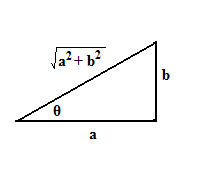
\includegraphics[scale=.8]{trigidentitypicture.png}
\caption{Using this picture, $C=\sqrt{a^2+b^2}$ and $tan(\theta)=\frac{b}{a}$.}
\label{fig:}
\end{figure}

Memorizing the picture, and noticing how the formula works is important for proving it and using it. For example, notice different amplitudes will work for this identity but Sine and Cosine need the same frequencies. \\

The next thing we should do is prove it. There are three proofs that are classic. The first is a high school proof, using the Cosine difference of two angles formula and convert the rest. However this proves the equation backwards implying it in the converse direction than how we will use it in Differential Equations. We usually want to simplify this into one trig function in differential equations and it would be a good idea to prove it in that direction. From obtaining the right side and substituting the left side if you will. Which does not help us since that high school proof proves it from right to left. \\

There are two techniques that prove it forwards (from left side to right). Here is a Calc 3 proof. We take advantage of two different ways to take the dot product of vectors 

\begin{equation*}
    acos(x)+bsin(x)=<a,b>\cdot<cosx,sinx> .
\end{equation*} 

Now we use the other definition of dot products, take the magnitudes, and Cosine definition which noticing $<a,b>$ has angle $\theta$ from the 3 O-clock position and $<cosx,sinx>$ is a unit vector of angle $x$ from the 3 O-clock position. So unit vector means magnitude is $1$ and it drops out. The dot product takes the difference of the two angles to find the included angle $x-\theta$. Thus it will become $|<a,b>| \cdot cos(x-\theta)$, assigning $|<a,b>|=C$ will complete the vector proof. \\

For the last proof, there is taking advantage of complex numbers. Watch us, with some magical foresight, cherry pick multiplying the following complex numbers.

\begin{equation*}
   (a-bi)(cosx+isinx) = (acosx+bsinx)+i(asinx-bcosx) 
\end{equation*}

Notice the real part is our left hand side of the identity, from here we convert this complex function on the left to polar coordinates and take the real part of the lefthand side. Notice that since $a+bi$ has angle $\theta$ then $a-bi$ has angle $-\theta$, also the modulus of $(a-bi)$ is Pythagorean theorem $\sqrt{a^2+b^2}$ then apply Euler's formula to the entire lefthand side to get

\begin{align*}
   (a-bi)(cosx+isinx) &= \sqrt{a^2+b^2} e^{-i\theta} e^{ix} \\
   (a-bi)(cosx+isinx) &= C e^{i(x-\theta)}.
\end{align*}

Taking the real part of $e^{i(x-\theta)}$ after using Euler's formula is just $cos(x-\theta)$, and that would complete our third proof.

\subsection{Two Ways to Complex Solutions} 
We will begin with an example demonstrating the last method and using the trig identity, then we will show another way to the solution and show these two ways actually produce the same solution set. We start with the Differential Equation

\begin{equation*}
    y'+4y'+5y=0.
\end{equation*}

This makes the Characteristic equation

\begin{equation*}
    r^2+4r+5=0.
\end{equation*}

Solutions will be by quadratic formula

\begin{equation*}
    r = \frac{-4 \pm \sqrt{-4}}{2} = -2 \pm i
\end{equation*}

Plugging into $e^{rt}$ we choose only the $e^{(-2+i)t}$ number, notice that

\begin{align*}
    e^{(-2+i)t} &= e^{-2t+it} \\
    e^{(-2+i)t} &= e^{-2t}e^{it} \\
    e^{(-2+i)t} &= e^{-2t}(cost+isint).
\end{align*}

The real part is $e^{-2t}cost$ and the imaginary part is $e^{-2t}sint$ which by the section above are shown that these are solutions to the Differential equation, by Principle of Superposition we get

\begin{equation*}
    y=c_1e^{-2t}cost+c_2e^{-2t}sint.
\end{equation*}

That would be our general solution. Lets make it an initial value problem, with $y(0)=1$ and $y'(0)=0$. The derivative of our general, not forgetting the product rule, is

\begin{align*}
    y' &= -2c_1e^{-2t}cos(t)-c_1e^{-2t}sin(t)-2c_2e^{-2t}sint+c_2e^{-2t}cost \\
    y' &= (-2c_1+c_2)e^{-2t}cos(t)+(-c_1-2c_2)e^{-2t}sint.
\end{align*}

Plugging in initial values we get

\begin{align*}
    1  &= c_1e^{-2\cdot0}cos(0)+c_2e^{-2 \cdot 0}sin(0) \\
    0 &= (-2c_1+c_2)e^{-2 \cdot 0}cos(0)+(-c_1-2c_2)e^{-2 \cdot 0}sin(0) \\
    1 &= c_1 \\
    0 &= (-2c_1+c_2) \\
    2 &=c_2.
\end{align*}

This gives us the solution $y=e^{-2t}(cost+2sint)$, we can now take advantage of our trig identity above to get

\begin{equation*}
    y = \sqrt{5}e^{-2t}cos(t-63.43^{\circ})
\end{equation*}

The angle there is approximate, notice that the trig identity allows us to visualize the solution in terms of just a transformation on Cosine, we have an amplitude $\sqrt{5}e^{-2t}$ that decreases to zero over time and a phase lag of about $63.43^{\circ}$, which shifts the basic cosine curve to the right by that amount. \\

With the steps of this method above considered, some questions naturally arise. Like why do we only use $e^{a+bi}$ and what happens if we use $e^{a-bi}$? In the end we would also get two solutions but they would not be two new solutions, consider that 

\begin{align*}
    y &= e^{(a-ib)t} \\
    y &= e^{at}e^{-ibt} \\
    y &= e^{at}(cos(-bt)+isin(-bt)) \\
    y &= e^{at}(cos(bt)-isin(bt)) \\
\end{align*}

The real part is still the same $e^{at}(cos(bt))$ but the imaginary part is $-e^{at}(sin(bt))$, or just the negative of the imaginary part was for $e^{a+bi}$. Given the difference there is only a constant multiple $-1$, the only adjustment would be made on the superposition where, replacing $c_2$ with $-c_2$, we get

\begin{equation*}
    y = c_1e^{at}(cos(bt))-c_2e^{at}(-sin(bt)).
\end{equation*}

However, since it is an arbitrary constant, it is still just as arbitrary with the change, which means the $r=a-bi$ creates no new solutions. \\

The next and most pressing question to ask is why did we take the real and imaginary part and hope each part would be a solution to the Differential Equation? When it would be more straightforward to use solutions $r=a+bi$ and $r=a-bi$ and put those into $e^{rt}$, take the Superposition and get

\begin{equation*}
    y = c_1e^{(a+bi)t}+c_2e^{(a-bi)t}.
\end{equation*}

The caveat here is the exponents do not let us conclude this to be a real number. Since each exponential makes a complex number, the only chance this solution will become fully real is if we allow $c_1$ and $c_2$ to be complex constants and figure out when they cancel the imaginary parts during the multiplication. Which means we should assign for each constant an arbitrary complex number, take Euler's Formula, multiply everything out into a fantastically long mess and set the imaginary part equal to zero to get our real solution. Although that would work, there is a better way that is shorter, cleaner and teaches a new insight along the way. \\

Consider changing a complex number $i$ to $-i$ to the above superposition, if after the transform the numbers are still equal we notice that is true only when the imaginary part is exactly zero. With this strategy, we can condition $c_1$ and $c_2$ to give us the real solutions we want. Let us take the complex conjugate of each constant to get

\begin{equation*}
 c_1e^{(a+bi)t}+c_2e^{(a-bi)t}  = \overline{c_1}e^{(a-bi)t}+\overline{c_2}e^{(a+bi)t}
\end{equation*}

Remember, this would create conjugates on the $c$'s as well and hence the bars. Notice this means that equating coefficients on $e^{(a+bi)t}$ makes $c_1 = \overline{c_2}$ and the coefficients equate on $e^{(a-bi)t}$ make $\overline{c_1} = c_2$. Notice that these two equations are redundant since

\begin{align*}
    c_1 &= \overline{c_2} \\
    \overline{c_1} &= \overline{\overline{c_2}} \\
    \overline{c_1} &= c_2.
\end{align*}

So since the two coefficient equations are redundant, let's just use $\overline{c_1} = c_2$. That means using $\overline{c+id}=c-id$ we have a real solution

\begin{equation*}
    y = (c+id)e^{(a+bi)t}+(c-id)e^{(a-bi)t}.
\end{equation*}

Many physicists and engineers use this as their solution. Finally one last curiousity arises before fully understanding the entire complex roots case, does this solution and our original solution $y = e^{at}(c_1cos(bt)+c_2sin(bt))$ differ at all, or are they two different solution sets? The answer is no, they are the same. We could show that by multiplying out our solution, use some messy algebra and conclude one is equal to the other, or we can again do something very clever to make its derivation simpler. Consider

\begin{align*}
    y &= (c+id)e^{(a+bi)t}+(c-id)e^{(a-bi)t} \\
    y &= e^{at}[(c+id)e^{ibt}+(c-id)e^{ibt}] \\
    y &= e^{at}[c(e^{ibt}+e^{ibt})+id(e^{ibt}-e^{ibt})] \\
\end{align*}

It is here where we need to recall some inverse equations derived from Euler's formula, that is $cos(b) = \frac{e^{ib}+e^{-ib}}{2}$ and $sin(b) = \frac{e^{ib}-e^{-ib}}{2i}$. With those substituted we get

\begin{align*}
    y &= e^{at}[2c\hspace{2 pt}cos(bt)+id(2i\hspace{2 pt}sin(bt)] \\
    y &= e^{at}[2c\hspace{2 pt}cos(bt)-2d\hspace{2 pt}sin(bt)].
\end{align*}

The arbitrary constants match up as $2c=c_1$ and $-2d=c_2$, which are just as arbitrary, after that this shows both solution forms are essentially two ways of describing the same family of functions. From here you can still use the trig identity as you wish to analyze the solution's behavior.

\subsection{Introducing the Wronskian}

It is at this point now that we know how to solve any case for Second Order Linear Homogeneous Equations with constant coefficients, the natural thing to do is fully deal with the study of the initial value part of the problems in more detail. First we will define initial value and boundary values, consider that an initial value is written of the form

\begin{align*}
    y(x_0) &= a \\
    y'(x_0) &= b.
\end{align*}

Notice that $y$ is the function, the second value is the derivative of $y$ and that we are plugging in the same $x$ value, the $x_0$ into both the function and the derivative. Geometrically speaking we have a point on the $xy$-plane and a line element of the slope, that is we know what one point looks like in the slope field already given we found that element by measuring for it in the physical problem. Though given that control, it is tempting to cherry pick what to measure to ensure $y(x_0)=0$ and $y'(x_0)=1$. For our case we will keep them $a$ and $b$ for the sake of being general. \\

After solving for one of the three cases, we have some form of the solution and its derivative to be

\begin{align*}
    y(x) &= c_1y_1(x)+c_2y_2(x) \\
    y'(x) &= c_1y'_1(x)+c_2y'_2(x).
\end{align*}

That means we plug in a value for $x$, specific number we will call $x_0$, this means

\begin{align*}
    y(x_0) &= c_1y_1(x_0)+c_2y_2(x_0) \\
    y'(x_0) &= c_1y'_1(x_0)+c_2y'_2(x_0).
\end{align*}

Flip it over and substitute for $a$ and $b$ to make a nice looking system.

\begin{align*}
    c_1y_1(x_0)+c_2y_2(x_0) &= a \\
    c_1y'_1(x_0)+c_2y'_2(x_0) &= b.
\end{align*}

Now we have a system, we solve for $c_1$ and $c_2$ with all other values have been given or calculated. This is now a Linear Algebra problem, to solve for a system of two equations with two unknowns we can do substitution, or elimination like we would in high school, but now that we are trying to solve for the general system, we will need matricies. That is we set up the matrix equation to be

\begin{align*}
    \left[
\begin{array}{cc}
y_1(x_0) & y_2(x_0) \\
y'_1(x_0) & y'_2(x_0) \\
\end{array}
\right]
\left[
\begin{array}{c}
c_1 \\
c_2 \\
\end{array}
\right] =
\left[
\begin{array}{c}
a \\
b \\
\end{array}
\right]
\end{align*}

We can solve for the vector of $c$'s by finding the inverse matrix of the matrix of $y$'s. The calculation of the inverse of a general $2x2$ matrix would be

\begin{align*}
    \left[
\begin{array}{cc}
a & b \\
c & d \\
\end{array}
\right]^{-1} = \frac{1}{ad-bc}
\left[
\begin{array}{cc}
d & -b \\
-c & a \\
\end{array}
\right]
\end{align*}

Recall $ad-bc$ is the determinant of a $2x2$ matrix, and that this determinant is denoted with bars such that $\left|
\begin{array}{cc}
a & b \\
c & d \\
\end{array}
\right|=ad-bc$. The important thing to notice is that if the determinant is zero, we divide by zero and therefore the inverse of that matrix does not exist, this is called a singular or degenerate matrix and this fact is true for the bigger square matrix cases as well. While in Linear Algebra, there were ways to skirt around solving a matrix equation that has a degenerate matrix, our concern in Differential Equations is when it does have an inverse. \\

Back to the problem, we know know the system is solvable, and shall be called a Fundamental Set of Solutions, when 

\begin{align*}
    \left|
\begin{array}{cc}
y_1(x_0) & y_2(x_0) \\
y'_1(x_0) & y'_2(x_0) \\
\end{array}
\right| \neq 0
\end{align*}

This is may be a determinant, but in the context of Differential Equations it is given another name, called the Wronskian, usually denoted as $W(y_1,y_2)$ and it usually calculated without plugging in an $x$ value like $x_0$, just so we can see what happens in any initial value problem for those solutions. The Wronskian can be generalized for bigger squares as well, the pattern is the same function on each column with the order indicated in the notation and each row number is the level of derivative of each function. \\

It will actually have more uses than just being a fancy word for helping us confirm if an initial value problem will work. Another thing about this is a non-zero determinant, is it confirms our solutions to be Linearly Independent by the Invertible Matrix Theorem from Linear Algebra. Conversely, if a zero determinant arises when plugging in the two solutions without an $x_0$ into each one, that means the solutions are Linearly dependant on each other. The usefulness of the Wronskian will arise when exploring in the tougher cases of Second Order Linear Equations.

\pagebreak

\subsection{Simplifying Initial Value Problems: Normalized Solutions}

After obtaining the solutions we come to realize all initial value problems are not created equal and some are used more than others. Consider the solution

\begin{equation*}
    y=c_1y_1+c_2y_2.
\end{equation*}

While they are a solution to solving a Differential Equation, other functions may be better for easing the effort it takes to solve the initial value problem. Let's say we had an alternative pair of linearly independent solutions for $y_1$ and $y_2$, let's call them $\mathcal{Y}_1$ and $\mathcal{Y}_2$. This process is called normalizing the solutions. For now we will normalize around $0$, that is we will consider the initial values $\mathcal{Y}_1(0)=1$, $\mathcal{Y'}_1(0)=0$, $\mathcal{Y}_2(0)=0$, and $\mathcal{Y}'_2(0)=1$. \\

Lets start with a basic example, notice the solutions to this differential equation are

\begin{align*}
    y"+y &= 0 \\
    y_1 &= cos(x) \\
    y_2 &= sin(x).
\end{align*}

Notice $cos(0)=1$ and its derivative with zero is $-sin(0)=0$ that makes $cos(x)=\mathcal{Y}_1$, notice $sin(0)=0$ and its derivative at zero is $cos(0)=1$ that makes $sin(x)=\mathcal{Y}_2$. \\

That is an easy case, but how about changing the solution to become normalized. Let us try it in this example

\begin{align*}
    y"-y &= 0 \\
    y_1 &= e^x \\
    y_2 &= e^{-x}.
\end{align*}

So here we can check and realize that they are not normalized yet, so lets put them in the general solution

\begin{align*}
    c_1e^x+c_2e^{-x} &= y_1 \\
    c_1e^x-c_2e^{-x} &= y'_1.
\end{align*}

To obtain $\mathcal{Y}_1$ use our initial values $\mathcal{Y}_1(0)=1$ and $\mathcal{Y'}_1(0)=0$ on the general solution.

\begin{align*}
    c_1e^0+c_2e^{-0} &= 1 \\
    c_1e^0-c_2e^{-0} &= 0 \\
    c_1+c_2 &= 1 \\
    c_1-c_2 &= 0 \\
    c_1=c_2 &= \frac{1}{2}.
\end{align*}

Therefore use the general solution $y_1$ with these values on the constants to make our $\mathcal{Y}_1$; that is $\frac{1}{2} e^x+ \frac{1}{2} e^{-x}$ which makes $\mathcal{Y}_1=\frac{e^x+e^{-x}}{2}$. Notice this is the Hyperbolic Sine Function. \\

We do this process again for $\mathcal{Y}_2$

\begin{align*}
    c_1e^0+c_2e^{-0} &= 0 \\
    c_1e^0-c_2e^{-0} &= 1 \\
    c_1+c_2 &= 0 \\
    c_1-c_2 &= 1 \\
    c_1 &= \frac{1}{2}. \\
    c_2 &= \frac{-1}{2}
\end{align*}

Therefore use the general solution $y_1$ with these values on the constants to make our $\mathcal{Y}_2$; that is $\frac{1}{2} e^x+ \frac{-1}{2} e^{-x}$ which makes $\mathcal{Y}_2=\frac{e^x-e^{-x}}{2}$. Notice this is the Hyperbolic Cosine Function. \\

To finally see the usefulness of doing this, let us write an initial value problem for particular values, that is $y(0)=y_0$ and $y'(0)=y'_0$. From here we can instantly write down the solution to the initial value problem in terms of $\mathcal{Y}_1$ and $\mathcal{Y}_2$, which would be $y=y_0\mathcal{Y}_1+y'_0\mathcal{Y}_2$. \\

Let us check why this is true. First lets show the first condition, $y(0)$ is true notice $y(0)=y_0\mathcal{Y}_1(0)+y'_0\mathcal{Y}_2(0)$, recall that $\mathcal{Y}_1(0)=1$ and $\mathcal{Y}_2(0)=0$, so $y(0)=y_0$ as desired. Again for the second condition, expect using the derivative this time. Notice $y'(0)=y_0\mathcal{Y}'_1(0)+y'_0\mathcal{Y}'_2(0)$, and recall $\mathcal{Y'}_1(0)=0$ and $\mathcal{Y'}_2(0)=1$. This makes $y'(0)=y'_0$ as desired. \\

Having the equations normalized allows us to circumvent initial value problems, though it does take a couple systems of equations to obtain it, the usefulness here is if in a study, you need to solve a large number of initial value problems, instead of solving that number of systems of equations, solve two of them to normalize it and instantly just write down the solution to each initial value problem afterwards. \\

\section{Undetermined Coefficients and Annihilator Method}

So far, the only kinds of Second Order Differential Equations we know how to solve are for Linear Homogeneous with constant coefficients, and that already took 3 cases of solutions and a load of pages of work to figure out. The work only gets more complicated from here when we slowly generalize solution techniques to expand for solving any kind of Second Order Linear Equation. Also the solution techniques will not be able to solve every kind of a certain equation it was intended to do. \\

Here we will cover Nonhonogeneous equations and the method of Undetermined Coefficients and its follow up Annihilator Method to solve most of that type. Some Linear Algebra shows itself for conceptual understanding but not needed for computation here. It will not solve all Nonhonogeneous unfortunately.

\subsection{Nonhonogeneous Equations Introduction}

We will begin our venture outside the basic second order realm with Nonhonogeneous equations. That is equations of the form

\begin{equation*}
    y"+Ay'+By=f(x).
\end{equation*}

As for what the $f(x)$ will physically mean when modeling a second order differential equation? For sake of an example, lets imagine say a mass-spring system with a dashpot, i.e. a thing that dampens an oscillator. Even though our form up above does not have a coefficient for $y"$, a model may have the need to make a coefficient there anyway. You can think of having a constant out front times $y"$ which can be thought of as acceleration if the original $y$ represents position. This will mean by Newtons Second Law that term means it is the force in the spring mass system. This force will be equal to the forces present in the system, the damping force that the dashpot supplies is $cy'$ which dampens the speed, the faster it is moving the more it slows down. The coefficient on $y$ is followed by Hooks law, or the spring constant, this force depends on position which causes a stretch or compressing spring. That is how the model normally works in a Homogeneous case, how does the $f(t)$ show up? That is modeled by being an outside force was not part of the system before, like hovering over the oscillator with an electromagnet or something. \\

There will be some terminology needed before we begin a solve for it, consider a Homogeneous form the equation 

\begin{equation*}
    y"+Ay'+By=0.
\end{equation*}

In terms of solving an Nonhonogeneous equation, the usual strategy is we will need to first solve the equation in the Homogeneous form. It comes with different names, two examples are the Associated Homogeneous Equation and the Reduced Equation. The solution for this equation will also have names, like $y_c=c_1y_1+c_2y_2$ with the subscript $c$ meaning the complementary solution. Another is $y_h=c_1y_1+c_2y_2$ with the subscript $h$ meaning the solution to the Associated Homogeneous Equation. After solving for the Homogeneous equation we still have to solve for the proposed Nonhonogeneous Equation yet. Usually the $f(t)$ will be some form of Exponentials, Sines and Cosines since those are usually the easier forms and will be typical outside forces that can occur out there in nature. We will need to find a particular solution for it and unfortunately to find it there is no hard set way. We will show some ways that have worked, in particular lets begin with just guessing. Let us start with an example starting with the equation

\begin{equation*}
    y"-4y'-12y = 3e^{5t}.
\end{equation*}

We start with solving the Homogeneous version which is a simple distinct root case

\begin{align*}
    y"-4y'-12y &= 0 \\
    r^2-4r-12 &= 0 \\
    r_1 = -2, \qquad r_2 &= 6.
\end{align*}

This gives us the general solution $y_c=c_1e^{-2t} + c_2e^{6t}$. 

\subsection{Method of Undetermined Coefficients}

Now that the reduced equation is solved, this is where luck and intuition will be involved in this solution method. We are going to make a guess at a particular solution to the Nonhonogeneous equation, given the complementary solution. \\

In our example our solution is in exponentials and the $y(t)$ is an exponential, it seems like guessing an exponential could work here, and in fact it will. The particular exponential to guess is $y_p=Ae^{5t}$ with $A$ being a parameter we will solve when we plug our guess. This concept of guessing a function but leaving the coefficient unknown so we can figure out what it should be is called the Method of Undetermined Coefficients. For other functions of $f(t)$ the guesses will become more involved and usually only works well when the $f(t)$ deals with sines, cosines, exponential, and combination sums of these. This method will not work well outside of that scope, but it will work in our example. \\

Let us plug $y=Ae^{5t}$ in and solve

\begin{align*}
    y"-4y'-12y &= 3e^{5t} \\
    25Ae^{5t}-20Ae^{5t}-12Ae^{5t} &= 3e^{5t}.
\end{align*}

Like we have done before, since $e^{5t}>0$ for all $t$, we can divide both sides by it easily enough

\begin{align*}
    25A-20A-12A &= 3 \\
    -7A &= 3 \\
    A = -&\frac{3}{7}
\end{align*}

Now we have a particular solution $y_p=-\frac{3}{7}e^{5t}$ that works. \\

A few questions arise from this, like why did we solve for the Homogeneous Equation and how did we really know to guess that particular solution? For guessing that particular solution, that comes with exposure to examples, anticipating what will happen when you plug your guess in and knowing your derivative rules well enough to do so and using previous examples to try sensible guess and some people even make tables of what should be good guesses to try. \\

Some classrooms will depend on intuition like this and make the struggle your own. Other rooms will break down many cases and make tables on what to guess for rules of thumb and they may or may not give you a table for guessing during test time. Lastly there is a construct of how to guess called the Annihilator Method, that method is meant learn how to make guesses for particular solutions feel more intuitive. We will not show the tabular method but we will cover the Annihilator Method later. \\

\subsubsection{Particular Plus Complement Solution}

Now the answer to the why solve the Homogeneous question will take some more math we can do right now. We will again look at this through a Linear Algebra approach. Consider that the Differential equation is written in linear operator form $Ly=f(t)$. The general solution to this should be $y=y_p+y_c$ or $y=y_p+c_1y_1+c_2y_2$. From here notice that to check to see if any solution of the above form is true then

\begin{align*}
    L(y_p + c_1y_1+c_2y_2)&=f(t) \\
    L(y_p)+L(c_1y_1)+L(c_2y_2)&=f(t) \\
    L(y_p)+c_1L(y_1)+c_2L(y_2)&=f(t) \\
    f(t)+c_1 \cdot 0+c_2 \cdot 0&=f(t) \\
    f(t) = f(t).
\end{align*}

This confirms all solutions of the form $y=y_p+c_1y_1+c_2y_2$ are true. Here we can see the usefulness of the complementary solution since it will not affect the left hand side from still being $f(t)$. Also notice we will not put an arbitrary constant, say $A$, next to $y_p$ since by linearity the operator would make the $f(t)$ turn into an $Af(t)$, which would not hold the equation true. Next what can also prove is showing that this solution is unique. Consider a new solution $u(x)$, notice that a new solution would mean that $L(u)=f(t)$ and we will show $u$ is not actually a new solution. To do this we will use the $y_p$ as our particular solution which means $L(y_p)=f(t)$. Consider that by subtracting the equations $L(u)=f(t)$ and $L(y_p)=f(t)$ from each other we see that

\begin{equation*}
    L(u-y_p) = 0.
\end{equation*}

From here we notice that $u-y_p$ satisfies the Homogeneous Differential Equation. The general form that covers all possible solutions of this equation is $c_1y_1+c_2y_2$. That means $u-y_p=c_1y_1+c_2y_2$ and therefore $u=y_p+c_1y_1+c_2y_2$. Notice now that $u$ is definitely not a new solution so we have this form of the solution is the general yet unique solution to the Linear Nonhonogeneous Differential Equation.

\subsubsection{Example Solution}

For those that struggle with the general proof can see it completed with our example. We have solution form of $y=y_p+y_c$ with $y_c=c_1y_1+c_2y_2$ and $y_p$ the particular, so we have a general solution solve of $y=-\frac{3}{7}e^{5t}+c_1e^{-2t} + c_2e^{6t}$. We will see if this plug back into our second order

\begin{equation*}
    y"-4y'-12y = 3e^{5t},
\end{equation*}

and see if it makes an identity. We have $y'=-\frac{15}{7}e^{5t}+-2c_1e^{-2t}+6c_2e^{6t}$ and $y"=-\frac{75}{7}e^{5t}+4c_1e^{-2t}+36c_2e^{6t}$, plugging this in becomes

\begin{align*}
    \left(-\frac{75}{7}e^{5t}+4c_1e^{-2t}+36c_2e^{6t} \right)& + \\
    -4\left(-\frac{15}{7}e^{5t}+-2c_1e^{-2t}+6c_2e^{6t} \right)& + \\
    -12\left(-\frac{3}{7}e^{5t}+c_1e^{-2t} + c_2e^{6t} \right)& = 3e^{5t}, \\
\end{align*}

Simplifying by combining like terms vertically we see it is in fact an identity

\begin{align*}
    \left(-\frac{75}{7}e^{5t}+4c_1e^{-2t}+36c_2e^{6t} \right)& + \\
    \left(\frac{60}{7}e^{5t}+8c_1e^{-2t}+-24c_2e^{6t} \right)& + \\
    \left(\frac{36}{7}e^{5t}+-12c_1e^{-2t} +-12c_2e^{6t} \right)& = 3e^{5t}, \\
    \frac{21}{7}e^{5t}\qquad +0c_1e^{-2t}  \qquad +0c_2e^{6t}& = 3e^{5t}.
\end{align*}

Notice how the complement solution exponentials will drop out to zero but our particular solution gets the needed Nonhonogeneous term anyway. It may seem strange to include the complement if it does not contribute to the solve whatsoever. Those with enough linear algebra knowledge will know what we mean when we claim that this will span all the possible solution space for this equation given the $c_1$ and $c_2$ parameters in play, where as only having the particular will not solve all possible Initial Value Problems that could follow.

\subsection{Annihilator Method Introduction}

A modified form of the Method of Undetermined Coefficients is called the Annihilator Method. This method will give us further insight about the lucky guesses for the form of the particular solution and eventually gives us an understanding where we effectively take all the guesswork out from the Undetermined Method. This also allows us to deal with linear equations of constant coefficients that deal with basically any size higher order differential equation. Some classrooms will teach the Annihilator and some will not. Even if your class does not teach them, learning this method even if outside the scope of your course will be vastly beneficial for executing Undetermined Coefficients, so might as well learn it anyway. \\
 
First lets consider the main but quite useful properties of the method. First we define what it means to annihilate a function. An operator, $P(D)$, annihilates a function $f$ if $P(D)[f]=0$. Lets see a function get annihilated
 
\begin{align*}
     (D-2)^2[te^{2t}]&=(D^2-4D+4)[te^{2t}] \\
     &= D^2[te^{2t}]-4D[te^{2t}]+4te^{2t} \\
     &= D[2(te^{2t})+e^{2t}]-4[2te^{2t}+e^{2t}]+4te^{2t} \\
     &= [2(2te^{2t}+e^{2t})+2e^{2t}]-8te^{2t}-4e^{2t}+4te^{2t} \\
     &= 4te^{2t}+2e^{2t}+2e^{2t}-4te^{2t}-4e^{2t} \\
     &= 4te^{2t}-4te^{2t}+4e^{2t}-4e^{2t} \\
     (D-2)^2[te^{2t}]&=0.
\end{align*}
 
This seems like a lot of work to do manually, which is why we will be tracking how general function forms can be annihilated. There are plenty of useful properties, this shortcuts a lot of work since we can bypass many product and chain rules using the rules below.

\vspace{10pt}

(i) Any polynomial of degree $m$, that is $p(t)=a_0+a_1t+a_2t^2+a_3t^3+...+a_mt^m$ can be annihilated by the operator $D^{m+1}$, or the $m+1$th derivative.

\vspace{10pt}

(ii) An exponential $e^{rt}$ can be annihilated by $(D-r)$.

\vspace{10pt}

(iii) A polynomial of degree $m$ times an exponential $(a_0+a_1t+a_2t^2+a_3t^3+...+a_mt^m)e^{rt}$ can be eliminated by $(D-r)^{m+1}$. This rule is demonstrated in the example above, where $a_0=0$, $a_1=1$, and $r=2$. Also since this is an exponential times a function, we could think in terms of the exponential shift rule here as well.

\vspace{10pt}

(iv) For $cos(r t)$ or $sin(r t)$, the annihilator would be $(D^2+r^2)$.

\vspace{10pt}

With these as the baseline, and expanding these rules further by executing the Exponential Shift Rule, we can cover many different kinds of functions that would show up in the Nonhonogeneous term. \\

We will show a few quick examples to demonstrate, notice taking $3$ derivatives of $t^2+8t+7$ will annihilate that expression to zero, demonstrating (i). Then $(D-3)[e^{3t}]$ is just $\frac{d}{dt}e^{3t}-3[e^{3t}]=3e^{3t}-3e^{3t}=0$, demonstrating (ii). Our example above demonstrates (iii). Then $sin(7t)$ will be knocked out with $(D^2+7^2)$ or that $\frac{d^2}{dt^2}sin(7t)-49sin(7t)=49sin(7t)-49sin(7t)=0$. \\

These 4 rules are not the only 4 Annihilator rules out there, there are more complicated forms like say multiplying various function forms together. Whatever depth your course goes, look at the source that teaches the method should make a list or table of all the possible rules they need eventually.

\subsection{Solving with Annihilators}

\subsubsection{General Description}

We can now show how to solve a Linear Nonhonogeneous Differential Equation with constant coefficients using the Annihilator method. Any equation of the form

\begin{equation*}
    P(D)y=g(t)
\end{equation*}

The method's script will work as follows:

\vspace{10pt}

(i) We will find the complementary solution or the solution of the homogeneous version of the differential equation, that works by just simplifying $P(D)$ by factoring usually and then look up which linearly independent functions get annihilated by each of the factors per the rules above or using the tables of annihilators given.

\vspace{10pt}

(ii) Find the annhilator of $g(t)$ the Nonhonogeneous term, take that operator to both sides of the equation to make it a homogeneous equation, this means that new annihilator operator will have to annihilate a function down to zero to make the Differential Equation hold. These will probably be your particular solutions.

\vspace{10pt}

(iii) Delete from the list of particular solutions, any solutions that already exist or are linearly dependent to the complementary solution.

\vspace{10pt}

(iv) Substitute your particular solutions and solve for their arbitrary constants that need to be solved.

\vspace{10pt}

(v) State your solution in terms of $y=y_c+y_p$ as per the usual method of Undetermined Coefficients.

\vspace{10pt}

\subsubsection{Example Solve}

Lets try this with what would otherwise be an unruly example of a really complicated differential equation

\begin{equation*}
    y'''-y''+y'-y=xe^{x}-e^{-x}+7.
\end{equation*}

Annihilators will make relatively quick work of this. First lets put the equation in operator form

\begin{equation*}
    (D^3-D^2+D-1)[y]=xe^{x}-e^{-x}+7.
\end{equation*}

Next we will solve the homogeneous version by fully factoring

\begin{equation*}
    (D^3-D^2+D-1)[y]=0.
\end{equation*}

We do this with factoring by grouping. It makes $(D^3-D^2+D-1)$ into $D^2(D-1)+(D-1)$ then factor out $(D-1)$ to get $(D^2+1)(D-1)$, therefore the equation looks like

\begin{equation*}
    (D^2+1)(D-1)[y]=0.
\end{equation*}

That means $(D^2+1)$ by rule (iv) the two functions $cos(x)$ and $sin(x)$ get annihilated by this operator. Also $(D-1)$ would annihilate $e^x$ per rule (ii). That means including superposition, our complementary solution would be

\begin{equation*}
    y_c=c_1cos(x)+c_2sin(x)+c_3e^x.
\end{equation*}

Three complementary solutions make sense since this is a third order differential equation after all and this completes step (i).

\vspace{10pt}

Next we must figure out how to annihilate $xe^{x}-e^{-x}+7$, one way to think of this is to annihilate each term, then see how the annihilators interact later. Consider $xe^x$, by rule (iii) gets annihilated by $(D-1)^2$. Then $-e^{-x}$, by rule (ii) gets annihilated by $(D+1)$, lastly $7$ is simple yet may be tough to see that rule (i) shows $D$ is enough there, that one with some common sense can be seen. If any of the multiple functions could be eliminated by the same operator, like if instead of $-e^{-x}$ we had $e^{x}$ that means we would choose $(D-1)$ there, but we already have $(D-1)^2$ in play which will not only annihilate $xe^x$ but also $e^x$ as well, keeping an eye out for lesser versions of functions is good to look for here, however none of our functions get taken out by the same operators so we have $(D-1)^2(D+1)D$ which will annihilate our Nonhonogeneous term. That is we should use this to help figure out our particular solutions, take this operator to both sides of the differential equation to get

\begin{align*}
    (D^3-D^2+D-1)[y]&=xe^{x}-e^{-x}+7 \\
    (D^2+1)(D-1)[y]&=xe^{x}-e^{-x}+7 \\
    [(D-1)^2(D+1)D](D^2+1)(D-1)[y]&=[(D-1)^2(D+1)D]xe^{x}-e^{-x}+7 \\
    (D+1)D(D^2+1)(D-1)^3[y]&=0 \\
\end{align*}

Now the Nonhonogeneous term is annihilated and we have a homogeneous equation with factored operators on the left, now lets use our rules and come up with all the linearly independent functions for $y$ that would be annihilated by one of the operators. Doing this for each operator consider the functions $e^{-x}$ for $(D+1)$, a constant function $A$ for $D$, the two $sin(x)$ and $cos(x)$ for $(D^2+1)$, then the trick one for $(D-1)^3$, this can annihilate $e^{x}$, $xe^{x}$, and $x^2e^{x}$. We could have chosen different polynomials of order $0$ $1$ and $2$ here in front of the exponential and that would also be a correct answer but then it would be harder to tell if each answer was linearly independent from each other, so we usually stick with simple $x$ raised to powers here. Given the solutions above are all linearly independent from each other we can move on to the next step. \\

Now lets compare our particular solution list to our complementary solution that is particulars $e^{-x}$, $A$, $sin(x)$, $cos(x)$, $e^{x}$, $xe^{x}$, and $x^2e^{x}$ with complementary $sin(x)$, $cos(x)$ and $e^{x}$. That means from the list of particular solutions we should throw out $sin(x)$, $cos(x)$ and $e^{x}$. That means our final list of particular solutions is now $A_1$, $e^{-x}$, $xe^{x}$, and $x^2e^{x}$, with each of these, tack on a constant, add them up and plug this back into the differential equation and solve for each constant, meaning we must plug in $y_p=A_1+A_2e^{-x}+A_3xe^{x}+A_4x^2e^{x}$ into the original equation and solve for $A_1$, $A_2$, $A_3$ and $A_4$. Doing this is long and messy and usually hand waived or by using computer software. To do it by hand, take the derivatives plug them in and equate coefficients and solve that system of equations. \\

When putting this into software we would achieve $A_1=-7$, $A_2=\frac{1}{4}$, $A_3=-\frac{1}{2}$, $A_4=\frac{1}{4}$, meaning the final particular solution is 

\begin{equation*}
    y_p=-7+\frac{e^{-x}}{4}-\frac{xe^{x}}{2}+\frac{x^2e^{x}}{4}.
\end{equation*}

Combining this with the complementary solution above, $y_c=c_1cos(x)+c_2sin(x)+c_3e^x$, we can now finally combine $y=y_c+y_p$ together to get our final answer to the differential equation is

\begin{equation*}
    y=c_1cos(x)+c_2sin(x)+c_3e^x-7+\frac{e^{-x}}{4}-\frac{xe^{x}}{2}+\frac{x^2e^{x}}{4}.
\end{equation*}

\section{Cauchy-Euler Equations}

We now branch into equations where the coefficients on the left side are no longer constant, we will not fully generalize the coefficients to arbitrary functions yet, that is still a ways away yet. Here we will learn to solve the Cauchy-Euler equation of the standard form

\begin{equation*}
    a_nx^ny^{(n)}+a_{n-1}x^{n-1}y^{(n-1)}+\ldots+a_2x^2y"+a_1xy'+a_0y=0.
\end{equation*}

This is with $y$ a function of $x$ and each $a$ is a parameter. This equation is generalized as a higher order equation but our methods for the second order version will translate to the higher orders all the same. There is two directions a classroom could go, sometimes a classroom will introduce both. We can either do a clever substitution that will turn any Cauchy-Euler into an equation with constant coefficients and solve via our previous methods. The second way is to make a clever guess for a solution, plug into this directly and run through the cases like we did in the constant coefficient section. We will demonstrate both.

\subsection{Substitute to Constant Coefficient}

Consider a general second order Cauchy Euler Equation of a standard form

\begin{equation*}
    x^2y"+axy'+by=0.
\end{equation*}

Now we perform a different kind of substitution, types we did in the past substituted for the function $y$. Now we will substitute an independent variable to make a new independent variable. We propose $x=e^t$. Now we make the necessary substitutes in

\begin{equation*}
    x^2\frac{d^2y}{dx^2}+ax\frac{dy}{dx}+by(x)=0,
\end{equation*}

and change the derivatives and independent variables in this with $t$s instead. We have $x=e^t$ means $\frac{dx}{dt}=e^t$ making

\begin{equation*}
    \frac{dy}{dx}=\frac{\frac{dy}{dt}}{\frac{dx}{dt}}=\frac{\frac{dy}{dt}}{e^t}=e^{-t}\frac{dy}{dt}.
\end{equation*}

So with $\frac{dy}{dx}=e^{-t}\frac{dy}{dt}$, as our way of substituting the first derivative in the equation, we strive for the second derivative. We  eventually obtain with a product rule

\begin{align*}
    \frac{d^2y}{dx^2}&=\frac{d}{dx}\left(\frac{dy}{dx}\right)=\frac{d}{dx}\left(e^{-t}\frac{dy}{dt}\right)=\frac{\frac{d}{dt}}{\frac{dx}{dt}}\left(e^{-t}\frac{dy}{dt}\right)=\frac{-e^{-t}\frac{dy}{dt}+e^{-t}\frac{d^2y}{dt^2}}{e^t} \\
    &=e^{-2t}\left(\frac{d^2y}{dt^2}-\frac{dy}{dt}\right).
\end{align*}

Substitute these two into the Cauchy-Euler, and also $x=e^t$ and $x^2=e^{2t}$

\begin{align*}
    x^2\frac{d^2y}{dx^2}+ax\frac{dy}{dx}+by&=0 \\
    e^{2t}e^{-2t}\left(\frac{d^2y}{dt^2}-\frac{dy}{dt}\right)+ae^te^{-t}\frac{dy}{dt}+by&=0 \\
    \left(\frac{d^2y}{dt^2}-\frac{dy}{dt}\right)+a\frac{dy}{dt}+by&=0 \\
    \frac{d^2y}{dt^2}+(a-1)\frac{dy}{dt}+by&=0.
\end{align*}

That is what it takes to convert. Since $a$ and $b$ are parameters, this is now a constant coefficient equation.

\subsubsection{Example}

Consider trying to solve

\begin{equation*}
    x^2y"+10xy'+20y=0.
\end{equation*}

We perform the substitution $x=e^t$, with $a=10$ and $b=20$ we skip through the derivation again and go straight to

\begin{equation*}
    \frac{d^2y}{dt^2}+9\frac{dy}{dt}+20y=0.
\end{equation*}

Now we just solve this constant coefficient equation per usual, we have $y(t)=e^{rt}$ and solve

\begin{align*}
    r^2e^{rt}+9re^{rt}+20e^{rt}&=0 \\
    (r^2+9r+20)e^{rt}&=0 \\
    (r+4)(r+5)&=0.
\end{align*}

With $r_1=-4$ and $r_2=-5$ we have the general solution to our substituted equation $y(t)=c_1e^{-4t}+c_2e^{-5t}$, now bringing back $x=e^t$, we have by some exponent laws or it could be done with equation inverse of $t=ln(x)$, we get

\begin{align*}
    y&=c_1e^{-4t}+c_2e^{-5t} \\
    y&=c_1\left(e^{t}\right)^{-4}+c_2\left(e^{t}\right)^{-5} \\
    y&=c_1x^{-4}+c_2x^{-5} \\
    y(x)&=c_1\frac{1}{x^{4}}+c_2\frac{1}{x^{5}}.
\end{align*}

Now our solution is for our original variable.

\subsection{Trial Solution}

Seeing the Cauchy-Euler solved with this clever substitution is nice because we can see the result without really having to guess the result like we had with our previous second order methods, regardless of if you see this method or not, eventually the guess of $y(x)=x^m$ would eventually come around. Mainly it seems like an intuitive guess once you see it plugged. We have

\begin{align*}
    y=x^m \qquad y'=mx^{m-1} \qquad y"&=m(m-1)x^{m-2} \\
    x^2y"\qquad +axy'\qquad +by&=0 \\
    x^2m(m-1)x^{m-2}+axmx^{m-1}+bx^m&=0 \\
    (m^2-m)x^m+amx^m+bx^m&=0 \\
    (m^2+(a-1)m+b)x^m&=0.
\end{align*}

Notice we need $x\neq 0$ to divide this one out so we will assume $x>0$ each time we guess this and cover the negative case later. With $a$ and $b$ parameters we have a quadratic to solve for the parameter, $m$ in our function guess. This is the characteristic equation for this function, it too will have 3 cases of solutions, distinct, repeated root and complex roots. We will covere those here.


\subsubsection{Distinct Roots Case}

The distinct root case is pretty straight forward, for example

\begin{equation*}
    x^2y"-3xy'+3y=0.
\end{equation*}

We start with $y=x^m$, $y'=mx^{m-1}$ and $y''=m(m-1)x^{m-2}$ per usual

\begin{align*}
    x^2m(m-1)x^{m-2}-3xmx^{m-1}+3x^m &= 0 \\
    m(m-1)x^2x^{m-2}-3mx^1x^{m-1}+3x^m &= 0 \\
    m(m-1)x^m-3mx^m+3x^m &= 0 \\
    (m(m-1)-3m+3)x^m &= 0 \\
    m(m-1)-3m+3 &= 0 \\
    m^2-m-3m+3 &= 0 \\
    m^2-4m+3 &= 0 \\
    (m-3)(m-1) &= 0 \\
    m = 3, 1&.
\end{align*}

The Cauchy-Euler will always have the law of exponents nicely combine into each term so you can factor out and divide away the $x^m$ every time, this will also happen for higher order Cauchy-Euler equations as well. Since we have distinct roots $m=1$ and $m=3$, that means $y_1=x$ and $y_2=x^3$ are fundamental solutions. Also even though the coefficients are not constant anymore, this second order equation is still linear, that means the Superposition principle still applies and the general solution will be

\begin{equation*}
    y=c_1x+c_2x^3.    
\end{equation*}

\subsubsection{Complex Roots Case}

We will see what the general solve is for this case, there will be parallels with the constant coefficient version of this. Consider a second Cauchy-Euler equation, we guess $y=x^m$ as the solve and say the solution to the Characteristic equation came out as $m=c\pm di$. Paralleling, we will only take the positive version of this so $y=x^{c+di}$, since this is not a useful form we use Euler's Formula turn it into

\begin{align*}
    x^{c+di} = e^{ln\left(x^{c+di}\right)} = e^{(c+di)ln(x)} &= e^{cln(x)}e^{dln(x)i} = e^{ln(x^c)}[cos(dln(x))+isin(dln(x))] \\
    x^c[cos(dln(x))+isin(d\cdot ln(x))] &= [x^c cos(dln(x))+i x^c sin(d\cdot ln(x))].
\end{align*}

Just like how it parallels before we could prove yet again that the real and imaginary part of this function will make the two real solutions we need. Superposition this and get general solution of

\begin{equation*}
    y=c_1 x^c cos(dln(x)) + c_2 x^c sin(dln(x)).
\end{equation*}

To see an example, we will solve

\begin{equation*}
    x^2y"+3xy'+4y=0.
\end{equation*}

Usual guess $y=x^m$, with $y'=mx^{m-1}$ and $y''=m(m-1)x^{m-2}$ per usual and we get

\begin{align*}
    x^2m(m-1)x^{m-2}+3xmx^{m-1}+4x^m &= 0 \\
    m(m-1)x^{m}+3mx^{m}+4x^m &= 0 \\
    m^2-m+3m+4 &= 0 \\
    m^2+2m+4 &= 0.
\end{align*}

This quadratic solves to $m=\frac{-2\pm \sqrt{4-4(1)(4)}}{2}=\frac{-2\pm 2\sqrt{-3}}{2}=-1\pm \sqrt{3}i$. With our general solve we use $c=-1$ and $d=\sqrt{3}$ to get

\begin{equation*}
    y=c_1 x^{-1} cos(\sqrt{3}ln(x)) + c_2 x^{-1} sin(\sqrt{3}ln(x)).
\end{equation*}

If this seems like there may be some holes in the argument, we suggest executing the check to see if this makes an identity, keep in mind there would be many product and chain rules happening here.

\subsubsection{Repeated Roots Case}

We will see that in this case when we get a $y_1(x)=x^{r_1}$ solution, we will have to work for the other one. There is a more general study for the concept called Reduction of Order we will justify later that will obtain this answer. Here we will just spoil the answer and say it takes $u(x)=ln(x)$ to have a second linearly independent solution. So in a case like

\begin{equation*}
    4x^2y"+8xy'+y=0.
\end{equation*}

We will get a repeated root solution like,

\begin{align*}
    4m(m-1)x^2x^{m-2}+8xmx^{m-1}+1&=0 \\
    4m^2+4m+1&=0 \\
    (2m+1)^2&=0 \\
    m = -\frac{1}{2}&.
\end{align*}

Then the full solution will become $y=c_1x^{-\frac{1}{2}}+c_2ln(x)x^{-\frac{1}{2}}$. For multiplicity 3 or higher continue using powers of log so $(ln(x))^n$ and increment that $n$ to get the linearly independent solutions you need.

\subsection{Other Variants}

Like with any other problem. There are possible curve balls along the way. Here are the ones that would show up for Cauchy-Euler.

\subsubsection{Third Order}

Here we see what it takes to have a result for a higher order Cauchy-Euler equation to show the generality of things. 

\begin{equation*}
    x^3\frac{d^3y}{dx^3}+5x^2\frac{d^2y}{dx^2}+7x\frac{dy}{dx}+8y=0.
\end{equation*}

Again we guess $y=x^m$ but take an extra derivative to plug in this time. So $\frac{dy}{dx}=mx^{m-1}$, $\frac{d^2y}{dx^2}=m(m-1)x^{m-2}$, and $\frac{d^3y}{dx^3}=m(m-1)(m-2)x^{m-3}$. Plug into the differential equation, combine like terms and factoring by grouping gets

\begin{align*}
    x^3m(m-1)(m-2)x^{m-3}+5x^2m(m-1)x^{m-2}+7xmx^{m-1}+8x^m &=0 \\
    x^m(m(m-1)(m-2)+5m(m-1)+7m+8) &= 0 \\
    x^m(m^3+2m^2+4m+8) = x^m(m+2)(m^2+4) &= 0.
\end{align*}

So $m_1=-2$, $m_2=2i$ and $m_2=-2i$, applying the complex root case and tack on $m_1$ to the superposition, our general solution will be

\begin{equation*}
    y=c_1x^{-2}+c_2cos(2\cdot ln(x))+c_3sin(2\cdot ln(x)).
\end{equation*}

\subsubsection{Negative $x$ Case}

Note how each time we guessed, we had to divide out an $x^m$ and assume $x\neq0$ to make the characteristic equation. Also in the repeated root and complex case the $x$ was a part of natural logs, meaning for those to be sensible we must assume when we begin the problem that $x>0$ to ensure our solutions do not break math. Here we try to consider what would happen if we need to solve this involving the $x<0$ interval instead. \\

What we will do to consider that is propose to substitute $w=-x$, with $x<0$, then $-x>0$ makes the new independent variable $w>0$. Now we have that $y(x)=y(-w)$. So we define $u(w)=y(-w)$. This leads to by chain rule $u'(w)=-y'(x)$ and $u"(w)=y"(x)$. This substitutes

\begin{align*}
    ax^2y"+bxy'+cy &= 0 \\
    a(-w)^2[u"(w)]+b(-w)[-u'(w)]+c u(w) &= 0 \\
    aw^2u"(w)+bwu'(w)]+cu(w) &= 0.
\end{align*}

This equation with $w>0$ now works the same way all our other Cauchy-Euler Equations have before. We will have distinct roots look like

\begin{align*}
    u(w) &= c_1w^{r_1}+c_2w^{r_2} \\
    y(x) &= c_1(-x)^{r_1}+c_2(-x)^{r_2} \qquad \text{ when } x<0.
\end{align*}

Comparing this solution to when we assume $x>0$, of $y(x) = c_1(x)^{r_1}+c_2(x)^{r_2}$, notice how this aligns with the absolute value function

\begin{equation*}
    |x|=\left\{
        \begin{array}{ll}
            x &  x \geq 0  \\
            -x & x < 0.
        \end{array}
    \right.
\end{equation*}

So that means the solution for all $x\neq0$ that will happen is

\begin{equation*}
    y=c_1|x|^{r_1}+c_2|x|^{r_2}
\end{equation*}

This thought process happens for repeated roots and complex roots too making the corresponding solution forms

\begin{align*}
    y=&c_1|x|^{r}+c_2|x|^{r}ln|x| \\
    y=&c_1|x|^{c}cos(d\cdot ln|x|)+|x|^{c}sin(d\cdot ln|x|).
\end{align*}

This Translates to our other curve ball problems. 

\subsubsection{Shifted Equation}

For a more general form of Cauchy-Euler, recall the concept of shifting $f(x)$ to the right by $a$, $f(x-a)$, this makes with parameter $x_0$

\begin{equation*}
    a(x-x_0)y"+b(x-x_0)y'+cy = 0.
\end{equation*}

The argument for this is pretty simple, we just name a new variable that substitutes for $x-x_0$, the fun of this form is derivatives involving this inside other functions will involve a chain rule but the derivative of $x-x_0$ in respect to $x$ will just be 1, so the substitution is pretty clean and the arguments basically run through the same but with $x-x_0$ instead. Note that for any $x\neq x_0$, using what we learned in the last section with absolute values, we will have the distinct, repeated and complex solutions of this shifted Cauchy-Euler to be of the forms

\begin{align*}
    y(x) =& c_1|x-x_0|^{r_1}+c_2|x-x_0|^{r_2} \\
    y(x) =& c_1|x-x_0|^{r}+c_2|x-x_0|^{r}ln|x-x_0| \\
    y(x) =& c_1|x-x_0|^{c}cos(d\cdot ln|x-x_0|)+|x-x_0|^{c}sin(d\cdot ln|x-x_0|).
\end{align*}

This again is with characteristic equation solutions of class distinct $r_1$, $r_2$, repeated root answer of $r$, and complex form of $c+di$.

\subsubsection{Nonhonogeneous}

For one more kind of curve ball consider a Cauchy-Euler but with a non-zero right side

\begin{equation*}
    x^2y"-xy'+y=ln(x).
\end{equation*}

The clever trick used here involves the callback to the substitution to the constant coefficient equation. Recall we had $x=e^t$ substitution making $x^2y"+axy'+by=0$ into $\frac{d^2y}{dt^2}+(a-1)\frac{dy}{dt}+by=0$ with the extra $ln(x)$ note that inverting our substitution also makes $ln(x)=t$ so our example with $a=-1$, $b=1$ really converts to

\begin{equation*}
    \frac{d^2y}{dt^2}-2\frac{dy}{dt}+y=t.
\end{equation*}

Now we have constant coefficients for an Nonhomogeneous equation, we can now do undetermined coefficients here. We will move things quicker with the Annihilator Method. We have the homogeneous solve to be

\begin{equation*}
    (D^2-2D+1)[y]=0
\end{equation*}

Factoring gets $(D-1)^2$, recall that functions that will get annihilated by that are $e^t$ and $te^t$, so these are the complementary solutions. Now to obtain the particular solve, we have to annihilate $t$ with $D^2$

\begin{align*}
    (D-1)^2[y]&=t \\
    D^2(D-1)^2[y]&=0
\end{align*}

This leads to again $e^t$ and $te^t$ already part of complement solution $y_c=c_1e^t+c_2te^t$. This leads to the new terms a constant function and a $t$ function that get annihilated by $D^2$, so the particular guess will be $y_p=A+Bt$. \\

So we plug that and derivatives $y'_p=B$ and $y"_p=0$ back into equation to solve

\begin{align*}
    y"-2y'+y&=t \\
    [0]-2[B]+[A+Bt]&=t \\
    (A-2B)+Bt&=0+1t.
\end{align*}

Equating coefficients here we have $A-2B=0$ and $B=1$, so that will make $A=2$, thus $y_p=2+t$ and our constant coefficient solution is

\begin{equation*}
    y(t)=y_c+y_p=c_1e^t+c_2te^t+2+t.
\end{equation*}

Recall this is not the Cauchy-Euler equation solve we started with yet. We substitute back from $t$ to $x$, using $x=e^t$ and $t=ln(x)$ to get our final solve

\begin{equation*}
    y(x)=c_1x+c_2xln(x)+2+ln(x).
\end{equation*}

That is a technique to solve a nonhomogeneous, we have more, consider if the right side had $sin(x)$, $cos(x)$ involved, those would not be as clean in the substitution here. Later we will learn to really dive deep into solving these kinds of problems with a technique called Variation of Parameters.

\pagebreak

\section{Reduction of Order Generalized} 

Note in the Cauchy-Euler solve in the repeated root case we skipped over derivations and just went with an answer, the concept of having one solution and needing to create a second linearly independent one out of thin air tends to be a need for these second and higher order equations. Here we will see more general techniques for obtaining a second solution if your usual method leaves you one solution short.

\subsection{Abel's Theorem Proofs}

\subsubsection{Reduction Proof}

Abel's Theorem is a formula that will obtain the second linearly independent solution from the first one for a general second order linear equation. This formula would also generalize to higher orders but we will just see the second order formula for now. \\

Consider a Differential Equation written in a slightly different looking form called Lagrange's notation

\begin{equation*}
    y"+ay'+by=0
\end{equation*}

with $a(x)$ and $b(x)$ are known functions and we have to solve for $y$, lets call the two solutions of this equation $y_1$ and $y_2$ we know $y_1$ but do not know $y_2$ yet. So we will try to obtain the solution like we have done before, in the constant coefficients section we guessed there would be a second solution by a guess of $y_2=u(x)y_1$, where we will solve for $u(x)$. Let's take this guess and plug back into the differential equation. We have 
\begin{align*}
   y_2 =& u\cdot y_1 \\
   y'_2 =& u \cdot y'_1 + y_1 \cdot u' \\
   y"_2 =& u \cdot y"_1 + 2y'_1\cdot u' + y_1 \cdot u".
\end{align*}

Substitute into the differential equation

\begin{align*}
    y"+ay'+by&=0 \\
    [u \cdot y"_1 + 2y'_1\cdot u' + y_1 \cdot u"] +a[u \cdot y'_1 + y_1 \cdot u'] + &b[u\cdot y_1] = 0 \\
    u[y"_1+ay'_1+by_1]+y_1u"+(2y'_1+ay_1)u'&=0.
\end{align*}

Note that since $y_1$ was our known solution that $[y"_1+ay'_1+by_1]=0$, this means we have

\begin{align*}
    y_1u"+(2y'_1+ay_1)u'&=0 \\
    y_1w'+(2y'_1+ay_1)w&=0.
\end{align*}

We make a substitution change of $u'=w$, thus $u"=w'$ so we have a separable first order equation. We execute the solve for $w(x)$ now

\begin{align*}
    y_1w' &= -(2y'_1+ay_1)w \\
    \frac{w'}{w} &= -\frac{(2y'_1+ay_1)}{y_1} \\
    \int \frac{w'}{w} dx &= \int -2\frac{y'_1}{y_1}-a dx \\
    ln(w) &= -2ln(y_1)- \int a(x) dx \\
    e^{ln(w)} &= e^{ln(y_1^{-2})} e^{-\int a(x) dx} \\
    w &= y_1^{-2}e^{-\int a(x) dx}.
\end{align*}

Now put back $w=u'$ and integrate that out, 

\begin{align*}
    u' &= \frac{e^{-\int a(x) dx}}{y_1^2} \\
    u(x) &= \int \frac{e^{-\int a(x) dx}}{y_1^2} dx.
\end{align*}

Note that we only want a single $u(x)$ so no point in needing the plus $C$s on the integrals. This makes the what we needed when we guessed $u(x)$, recall our second solution was $y_2(x)=u(x)y_1(x)$, so our final solution is

\begin{equation*}
    y_2(x)=y_1 \int \frac{e^{-\int a(x) dx}}{y_1^2} dx.
\end{equation*}


\subsubsection{Wronskian Proof}

Here we see the proof again but involving Wronskians. As introduced in the Introduction to Second Order Equations the point of the Wronskian was to essentially help us with solving the initial value problem, it tells us when we cannot figure out the system of equations that come from the initial values and allows to anticipate what initial values we could measure and solve. It also allows us to confirm that the two functions are Linearly Independent by being a non-zero answer. There are other uses and cameos that the Wronskian will make in Differential Equations, like in the Variation of Parameters formula in the next section. For now we will see it can reprove Abel's Theorem as well. \\

We will prove this Wronskian solution method is true for the Second Order case. Again, Consider a second order linear Differential Equation written in a slightly different looking form than last proof

\begin{equation*}
    y"=ay'+by
\end{equation*}

with $a(x)$ and $b(x)$ are known functions and we have to solve for $y$, again we call the two solutions of this equation $y_1$ and $y_2$ we know $y_1$ but do not know $y_2$ yet. Notice the Wronskian of those two solutions will be

\begin{equation*}
    W(x)=y_1y'_2-y_2y'_1.
\end{equation*}

Now we will play around with it and find some interesting properties of it, let us start with differentiating the Wronskian, which is

\begin{align*}
    W'(x)&=y'_1y'_2+y_1y''_2-(y'_2y'_1+y_2y''_1) \\
    W'(x)&=y_1y''_2-y_2y''_1.
\end{align*}

Remember that $y_1$ and $y_2$ obey to the differential equation, we can take these double derivatives and see that in the differential equation they are $y''_1=ay'_1+by_1$ and $y''_2=ay'_2+by_2$. Substitute that and see

\begin{align*}
    W'(x)&=y_1(ay'_2+by_2)-y_2(ay'_1+by_1) \\
    W'(x)&=ay_1y'_2+by_1y_2-ay_2y'_1-by_2y_1 \\
    W'(x)&=ay_1y'_2-ay_2y'_1 \\
    W'(x)&=a(y_1y'_2-y_2y'_1) \\
    W'(x)&=a(x)W(x).
\end{align*}

We have ourselves a Separable Differential equation here. We solve that to get

\begin{align*}
    W'(x)&=a(x)W(x) \\
    \int \frac{W'(x)}{W(x)} dx &= \int a(x) dx \\
    ln\left(W(x)\right) &= \int a(x) dx \\
    W(x)&=e^{\int a(x) dx}.
\end{align*}

Notice we only want a single second order solution so we ignore plus $C$s. Seeing how we know solution $y_1$ but not $y_2$ yet, lets expand the Wronskian on the left and solve for $y_2$.

\begin{align*}
    y_1y'_2-y_2y'_1&=e^{\int a(x) dx} \\
    y'_2-\frac{y'_1}{y_1}y_2&=\frac{e^{\int a(x) dx}}{y_1}.
\end{align*}

This equation is a first order linear equation with all functions given except for $y_2$. We will use integrating factors to solve. Note that the integrating factor is

\begin{equation*}
    e^{\int -\frac{y'_1}{y_1}dx}=e^{-ln(y_1)}=e^{ln(y_1^{-1})}=y_1^{-1}=\frac{1}{y_1}.
\end{equation*}

Multiply this to both sides and solve for $y_2$,

\begin{align*}
    \frac{1}{y_1}y'_2-\frac{y'_1}{y_1^2}y_2&=\frac{e^{\int a(x) dx}}{y_1^2} \\
    \left[\frac{1}{y_1}\cdot y_2\right]'&=\frac{e^{\int a(x) dx}}{y_1^2} \\
    \int \left[\frac{1}{y_1}\cdot y_2\right]'dx&=\int \frac{e^{\int a(x) dx}}{y_11^2} dx \\
    \frac{1}{y_1}\cdot y_2&=\int \frac{e^{\int a(x) dx}}{y_1^2} dx \\
    y_2&=y_1 \int \frac{e^{\int a(x) dx}}{y_1^2} dx.
\end{align*}

There is our final form again. Notice our standard form in this proof had the middle term with $a(x)y'$ on the right side instead of the left, making it a negative function of our proof's standard form. This translates when comparing the formula where their $\int a(x) dx$ had a negative sign. Therefore this proves the same formula if our standard forms were the same. This proof technique generalizes to higher order equations easier than our first proof technique. It would take a lot of linear algebra to go higher order though so we will not show it here.

\subsection{Cauchy Euler Repeated Root Example}

Recall we did not derive the second solution in the repeated root case of the Cauchy-Euler equation. Now to write the general form of the repeated root case. Assume we had a solve of $m=r$ with $r$ multiplicity 2. That would have a quadratic of $(m-r)^2=0$ or $m^2-2r+r^2=0$. Recall we would solve $x^2y"+axy'+by=0$ by guessing $y=x^m$, with $y'=mx^{m-1}$ and $y"=m(m-1)m^{m-2}$ and obtain quadratic

\begin{align*}
    (m(m-1)+am+b)x^m &= 0 \\
    m^2+(a-1)m+b &= 0.
\end{align*}

Matching coefficients with $m^2-2r+r^2=0$, we have $a-1=2r$ and $b=r^2$. We will be using $a=2r+1$ in our solve later. \\

Now that we have the restrictions that will ensure the repeated root case happens. We now put our Cauchy-Euler into the form

\begin{equation*}
    y"+\frac{a}{x}y'+\frac{b}{x^2}y=0.
\end{equation*}

This is the same standard form as our first proof so we will use that formula, we divide by $x^2$ to ensure coefficient of $y"$ is one. Remember back all the way back then $a$ and $b$ are parameters now. In our general reduction of order proofs $a$ and $b$ were functions of $x$. So in repeated roots fashion we will have a first solution of $y_1(x)=x^{r}$ with $r$ being the root of the quadratic solve that has multiplicity 2. So to obtain the second linearly independent solution, we apply $a(x)=\frac{a}{x}$ to Abel's Formula to get

\begin{align*}
    y_2(x) &= y_1 \int \frac{e^{-\int a(x) dx}}{y_1^2} dx \\
    y_2(x) &= x^r \int \frac{e^{-\int \frac{a}{x}}}{(x^r)^2} dx = x^r \int \frac{e^{-aln(x)}}{(x^r)^2} dx \\
    &= x^r \int \frac{e^{ln(x^{-a})}}{x^{2r}} dx = x^r \int x^{-a}x^{-2r} dx \\
    &= x^r \int x^{-a-2r} dx.
\end{align*}

Now recall we had a restriction of $a=2r+1$ to keep our equation in the repeated root case. This makes $\int x^{-a-2r} dx=\int x^{-(2r+1)-2r} dx=\int x^{-1}$. Now we have

\begin{equation*}
    y_2(x) = x^r \int \frac{1}{x} = x^r \cdot ln(x)
\end{equation*}

This matches with the solution we claimed to be true in that section. Now in order to say solve a 3rd order equation and have two of them be repeated roots, we would need to derive the 3rd order Abel Formula, using two known solutions to obtain the third. If we did go through all that math, we would realize if we had a root of multiplicity 3, the solutions would be $x^r$, $x^r\cdot ln(x)$ and $x^r\cdot [ln(x)]^2$ and this concept would keep on going. This method helps with more complicated methods of this, for example some second and higher order equations would not be solvable by elementary functions, of which we would solve equations using long winded Taylor Series methods. Those are painful and so using Abel's Formula to solve would cut down on some work.

\pagebreak

\section{Variation of Parameters}

\subsection{General Solve}

While the Method of Undetermined Coefficients will work in certain cases, we can make a second stab at equations we cannot with that method with a more powerful but a bit more invested method called Variation of Parameters. This method also finds a particular solution to an Nonhonogeneous Equation like in Undetermined Coefficients. Though this method can solve some equations of the form

\begin{equation*}
    p(t)y"+q(t)y'+r(t)y=g(t)
\end{equation*}

Normally the Method of Undetermined Coefficients works for most cases of constant coefficients, but this method will work in more cases of that with a wider selection of $g(t)$ but also will sometimes work in cases without constant coefficients as well. The differences of the method start with the reduced Homogeneous equation, in Undetermined coefficients it was advisable to have the complementary solution to help make a good guess, but it could technically be done without. For Variation of Parameters we absolutely need to have it, for many introductory problem sets they are usually provided for you, since some complementary solutions can be pretty creative especially for examples that have functions instead of constant coefficients. That means for now, let us consider we have the general solution to the Associated Homogeneous Equation of the form

\begin{equation*}
    y_c(t)=c_1y_1(t)+c_2y_2(t).
\end{equation*}

Also $y_1$ and $y_2$ were particular solutions in the Homogeneous case. Given the new context of a looming Nonhonogeneous equation to solve, the role of those two functions change so we will change their name to indicate this, from Particular Solutions to Fundamental Solutions. \\

The method we are about to present took some luck to find but after introduction it will become a much more straightforward process than Undetermined Coefficients to solve actual examples. This method was founded by two prodigy Mathematicians, first introduced by Leonhard Euler, then the method finally completed over fifty years later by Lagrange. With some parameter like functions $u_1$ and $u_2$, we hope that the solution will look of the form

\begin{equation*}
    Y_p(t)=u_1(t)y_1(t)+u_2(t)y_2(t).
\end{equation*}

Given we are presenting this, the luck of this guess will pan out here. Notice we have two unknown functions that we have to solve. That means we will need two equations of each of them to ensure a solution for each one. Consider plugging this solution back into the Differential Equation, before we do let us take some derivatives

\begin{equation*}
    Y'_p(t) = u'_1y_1+u_1y'_1+u'_2y_2+u_2y'_2.
\end{equation*}

The first equation will come out of nowhere, we have a second order equation to input but to make taking the second derivative easier we are going to assume that 

\begin{equation*}
    u'_1y_1+u'_2y_2=0
\end{equation*}

This simplifies the second derivative, but we have no idea if the solution will still pan out, however improbable this solution method is, this assumption by shear luck will happen to work out nicely. Hence why this method took an extra fifty years until Lagrange got the idea to try this assumption. So make those two terms zero and differentiate

\begin{align*}
    Y'_p(t) &= u_1y'_1+u_2y'_2 \\
    Y"_p(t) &= u'_1y'_1+u_1y''_1+u'_2y'_2+u_2y''_2.
\end{align*}

Now we have our three forms, plug each derivative into the Differential equation, remember to use the simpler first derivative, to obtain

\begin{equation*}
    p(t)\left(u'_1y'_1+u_1y''_1+u'_2y'_2+u_2y''_2\right)+q(t)\left(u_1y'_1+u_2y'_2\right)+r(t)\left(u_1(t)y_1(t)+u_2(t)y_2(t)\right)=g(t).
\end{equation*}

We rearrange the terms to get

\begin{equation*}
    p(t)\left[u_1'y'_1+u'_2y'_2\right]+u_1\left[p(t)y''_1+q(t)y'_1+r(t)y_1 \right] + u_2\left[p(t)y''_2+q(t)y'_2+r(t)y_2 \right] = g(t).
\end{equation*}

We arrange it in this manner so we can see that $p(t)y''_1+q(t)y'_1+r(t)y_1$ and $p(t)y''_2+q(t)y'_2+r(t)y_2$ are present in the left side of our initial differential equation. Also since $y_1$ and $y_2$ are solutions to the homogeneous version that means each of those two expressions are $0$. With those terms dropping out we have a simplified version of the following.

\begin{align*}
    p(t)\left(u_1'y'_1+u'_2y'_2\right)+u_1[0]+u_2[0]&=g(t) \\
    \left(u_1'y'_1+u'_2y'_2\right)&=\frac{g(t)}{p(t)}.
\end{align*}

Recall that $p(t)$ is the coefficient of the $y"$ term from the initial differential equation. We are going to assume it is $1$ to simplify this equation to be

\begin{equation*}
    u_1'y'_1+u'_2y'_2=g(t).
\end{equation*}

This will be the second equation in our system to solve for $u_1$ and $u_2$. This is the minimum we need  to be able to solve using this method. That means the solution technique is the following: \\

1) Put into standard form and divide out coefficient of $y"$ since we assumed it was $1$. \\

2) Find the Fundamental solutions aka two particular solutions, $y_1$ and $y_2$, to the homogeneous version if they have not been given. \\

3) Solve the following system of equations for $u'_1$ and $u'_2$ 

\begin{align*}
    u'_1y_1+u'_2y_2&=0 \\
    u_1'y'_1+u'_2y'_2&=g(t).
\end{align*}

4) After finding $u'_1$ and $u'_2$, integrate both to plug into the particular solution $y_p=u_1y_1+u_2y_2$, which will be our answer. \\

Some textbooks will solve the step 3 system of equations in general. Like with the Integrating Factors Method, this means you can either use the process above or simply plug and chug into the final formula which we will derive now. First solve for $u'_1$ on the first equation, then substitute back in the second equation and solve.

\begin{align*}
    u'_1 = -\frac{u'_2y_2}{y_1}& \\
    \left(-\frac{u'_2y_2}{y_1}\right) y'_1 + u'_2y'_2&=g(t) \\
    u'_2 \left(y'_2-\frac{y_2y'_1}{y_1} \right) &=g(t) \\
    u'_2 \left(\frac{y_1y'_2-y_2y'_1}{y_1} \right) &=g(t) \\
    u'_2 = \frac{y_1g(t)}{y_1y'_2-y_2y'_1}&.
\end{align*}

We have now solved the expression for $u'_2$, plug this into the top equation that isolated $u'_1$ to get

\begin{equation*}
    u'_1 = -\frac{y_2g(t)}{y_1y'_2-y_2y'_1}.
\end{equation*}

Notice in each solution here we have a denominator of $y_1y'_2-y_2y'_1$, this is actually the Wronskian, $W(y_1,y_2)$ of $y_1$ and $y_2$, also since these two are Fundamental Solutions, then they are Linearly Independent. That means by the Invertible Matrix Theorem the Determinant, or Wronskian of this, is non-zero. Therefore the denominator of each of the fractions will not inhibit finding the solution. Though consider the rest of the solve, substituting for $W(y_1,y_2)$ and integrating as stated from step 4, we get

\begin{align*}
    u_1(t) &= -\int \frac{y_2g(t)}{W(y_1,y_2)} dt. \\
    u_2(t) &= \int \frac{y_1g(t)}{W(y_1,y_2)} dt.
\end{align*}

In short, this means the particular solution $y_p=u_1y_1+u_2y_2$ of the Nonhonogeneous Differential Equation, given $y_1$ and $y_2$ are solutions to the Homogeneous version, is

\begin{equation*}
    y_p = -y_1\int \frac{y_2g(t)}{W(y_1,y_2)} dt + y_2 \int \frac{y_1g(t)}{W(y_1,y_2)} dt.
\end{equation*}

This formula we can plug and chug if we do not want to use the four step process above. Here the caveat is can we integrate both of these integrals, many times they are nasty and sometimes unsolvable. With this and also being unable to find two fundamental solutions in the first place will be where the method could fail to deliver.

\subsection{Variation of Parameters Example}

Lets do a simple yet creative example of the method, we will use the process but plugging the formula will get the same answer too. Consider the Differential Equation

\begin{equation*}
    x^2y"-3xy'+3y=4x^7.
\end{equation*}

The Associated Homogeneous Equation is

\begin{equation*}
    x^2y"-3xy'+3y=0.
\end{equation*}

This Homogeneous Equation also is a Cauchy-Euler Equation, notice how we solved this particular equation in that section, so we steal that fundamental solution of $y_1=x$ and $y_2=x^3$. Next we need our equation in standard form so the coefficient of $y"$ is one, that is

\begin{equation*}
    y''-\frac{3}{x}y'+\frac{3}{x^2}y=4x^5.
\end{equation*}

Next we must solve the system of equations that were derived above, with derivatives of of the fundamental solutions being $y'_1=1$ and $y'_2=3x^2$, we solve the first equation for $u'_1$ and plug it into the second equation, we will obtain

\begin{align*}
    u'_1x+u'_2x^3 &= 0 \\
    u'_1(1)+u'_2(3x^2) &= 4x^5. \\
    u'_1&=-u'_2x^2 \\
    (-u'_2x^2)+u'_2(3x^2) &= 4x^5. \\
    u'_2(2x^2)&=4x^5. \\
    u'_2&= 2x^3. \\
    u'_1 &= -(2x^3)x^2 \\
    u'_1 &= -2x^5.
\end{align*}

Integrating $u'_1$ and $u'_2$ that means $u_1=-\frac{x^6}{3}$, and $u_2=\frac{x^4}{2}$. Putting these terms and the Fundamental Solutions back into $y_p=u_1y_1+u_2y_2$ will become

\begin{align*}
    y_p &= \left(-\frac{x^6}{3}\right)(x)+\left(\frac{x^4}{2}\right)(x^3) \\
    y_p &= \left(-\frac{x^7}{3}\right)+\left(\frac{x^7}{2}\right) \\
    y_p &= \frac{x^7}{6}.
\end{align*}

That is the particular solution to the Nonhonogeneous Differential Equation, then the general solution to it is

\begin{equation*}
    y=\frac{x^7}{6}+c_1x+c_2x^3.
\end{equation*}

This is our complete general form that solves $x^2y"-3xy'+3y=4x^7$. \\

\subsubsection{With Integrals}

Notice how using the integral formulas will also get the some answer, note that $W(y_1,y_2)=y_1y'_2-y'_1y_2=(x)(3x^2)-(1)(x^3)=2x^3$, thus we have

\begin{align*}
    u_1(x) &= -\int \frac{y_2g(x)}{W(y_1,y_2)} dx. \\
           &= -\int \frac{(x^3)(4x^5)}{2x^3} dx \\
           &= -\int 2x^5 dx \\
           &= -\frac{1}{3}x^6. 
\end{align*}

Then also substituting for $u_2$,

\begin{align*}
    u_2(x) &= \int \frac{y_1g(x)}{W(y_1,y_2)} dx \\
           &= \int \frac{(x)(4x^5)}{2x^3} dx \\
           &= \int 2x^3 dx \\
           &= \frac{1}{2}x^4.
\end{align*}

Substitute for $y_p=u_1(x)y_1(x)+u_2(x)y_2(x)=[-\frac{1}{3}x^6](x)+[\frac{1}{2}x^4](x^3)=\frac{x^7}{6}$ to get the same particular solution we had solved before.

\pagebreak

\section{Nonhonogeneous $D$ operator rules (Optional)}

Here we truly dive into the operator notation of Differential Equations, like $(D-4)y(x)$. Diving fully into this thinking reveals many great insights into solving Inhomogenous Differential Equations. This requires loads of abstract thinking in Operator Notation and plenty of abilities involving complex numbers and functions, as such almost all classrooms will not introduce this method because they do not want to teach the fundamentals of complex analysis in this class. For those with the ability to work in complex functions this method reveals some extra insights into solving Nonhonogeneous higher order Equations.

\subsection{Exponential Input Theorem Introduction}

For the Method of Undetermined Coefficients, the whole guessing a function with an unknown coefficient is not great, but we can create some predictability for when $f(t)$ can be written as an exponential function. Consider we are in the realm of constant coefficients with an Nonhonogeneous Equation which in the general form looks like

\begin{equation*}
    y"+Ay'+By=f(x).
\end{equation*}

From here let us again rewrite it in terms of operators that would be

\begin{equation*}
    (D^2+AD+B)y=f(x)
\end{equation*}

From here we will not use the operator $L$ to summarize it, this time we will use $p(D)$ which stands for a polynomial in terms of the derivative operator. We write it this way because we will show that method below will work for any order polynomial whether it is 2nd order like above or a higher order. Now let us begin by taking a $p(D)$ to a complex exponential $e^{\alpha x}$ with the $\alpha$ being a complex number. That means $p(D)e^{\alpha x} = p(\alpha)e^{\alpha x}$ by the chain rule, and this equation is called the Substitution Rule. To interpret $p(\alpha)$, consider if $p(D)=D^2+AD+B$, then $p(\alpha)$ means to replace $D$ with the complex number $\alpha$ so that $p(\alpha)=\alpha^2+A\alpha+B$. \\

We can prove the Substitution Rule is true pretty easily, we will just show it for the example. Consider $(D^2+AD+B)e^{\alpha x}=D^2e^{\alpha x}+ADe^{\alpha x}+Be^{\alpha x}$. This becomes $\alpha^2e^{\alpha x}+A\alpha e^{\alpha x} + Be^{\alpha x}=(\alpha^2+A\alpha + B)e^{\alpha x}$, and that is a proof for $p(D)e^{\alpha x}=p(\alpha)e^{\alpha x}$ in a nutshell. \\

Now we have what we need to introduce something important called the Exponential Input Theorem. The theorem states that for a differential equation like $p(D)y = e^{\alpha x}$, the particular solution for that equation will be $y_p=\frac{e^{\alpha x}}{p(\alpha)}$. \\

The proof for this is simple really, plug it into the equation and see if $p(D)y_p = e^{\alpha x}$ holds true. We start with $p(D)\frac{e^{\alpha x}}{p(\alpha)} = p(\alpha)\frac{e^{\alpha x}}{p(\alpha)}$. This is true because first of all the $p(D)e^{\alpha x}=p(\alpha)e^{\alpha x}$ is the substitution rule, but what about the $p(\alpha)$ in the denominator on the left side? That is a constant, seeing how the $D$ operator is differentiating in respect to $x$ and not the complex number $\alpha$, also $p(D)=L$ means it is linear so we can allow a constant like $\frac{1}{p(\alpha)}$ to go along with the ride. Now that the equation above is justified we can cancel the $p(\alpha)$ on top and bottom and have just $p(D)\frac{e^{\alpha x}}{p(\alpha)} = e^{\alpha x}$, as desired. Of course the caveat is $p(\alpha) \neq 0$ to avoid zero division.

\subsection{Exponential Input Theorem Example}

Let's show the power of the Exponential Input Theorem, this will assume some knowledge of complex numbers, namely Euler's formula and how to divide complex numbers. We begin with example

\begin{equation*}
    y"-y'+2y=10e^{-x}sin(x).
\end{equation*}

Looks like a complicated guess for Undertermined Coefficients, however we will take advantage of Euler's formula, we complexify the right side to be

\begin{equation*}
    (D^2-D+2)\tilde{y}=10e^{(-1+i)x}.
\end{equation*}

Notice the imaginary part of $e^{(-1+i)x}$ is $e^{-x}sin(x)$. Since the equation changed forms the solution for the second equation will not be the answer, so we call it $\tilde{y}$ to show we will still need to take the imaginary part of it after we obtain it. Now we have an $\alpha =-1+i$, the right side is in exponential form, from the Exponential Input theorem we now can just jump straight to the solution, which is 
\begin{equation*}
    \tilde{y_p}=\frac{10e^{(-1+i)x}}{(-1+i)^2-(-1+i)+2}.
\end{equation*}

Now that we have $\tilde{y}$ remember that we solved the complexified differential equation, we need our original imaginary part of the right side, in complex number land means we need the imaginary part of that solution. This will take some work to accomplish that so lets begin with simplifying the denominator to

\begin{equation*}
    \tilde{y_p}=\frac{10e^{(-1+i)x}}{3-3i}.
\end{equation*}

We are dividing two complex numbers, factor out a $3$ and then multiply top and bottom by the conjugate to make the donominator real and get

\begin{align*}
    \tilde{y_p} &=\frac{10}{3}\frac{(1+i)}{(1-i)(1+i)}e^{(-x+ix)} \\
    \tilde{y_p} &=\frac{10}{3}\frac{(1+i)}{2}e^{-x}(cos(x)+isin(x)).
\end{align*}

Notice the law of exponents and writing out Euler's Formula here. Our end goal is to find the imaginary part here since that is our real $y_p$ answer. We notice we have to multiply $(1+i)(cos(x)+isin(x))$, we will cherry pick the parts we know will be imaginary, which is $cos(x)+sin(x)$. This means

\begin{equation*}
    y_p = \frac{5}{3}e^{-x}(cos(x)+sin(x))
\end{equation*}

We take advantage of the trig identity shown in the Introduction to Second Order paper, so $cos(x)+sin(x)=\sqrt{2}cos(x-\frac{\pi}{4})$ which then simplifies the solution to be

\begin{equation*}
    y_p = \frac{5\sqrt{2}}{3}e^{-x}cos(x-\frac{\pi}{4}).
\end{equation*}

\subsection{Exponential Shift Rule}

In the Exponential Input Theorem we assumed that $p(\alpha) \neq 0$. An example of an equation that would not work up there would be $y"-3y'+2y=e^x$, notice the coefficient of $x$ in the exponent is $\alpha=1$. Also we can see that $p(D)=D^2-3D+2$, that means $p(\alpha)=\alpha^2-3\alpha+2=(\alpha-1)(\alpha-2)$, therefore $p(1)=0$. Because of examples like that, it is time to consider if $p(\alpha)=0$. We will begin with considering an analog of the Substitution Rule that will be useful here. This is called the Exponential Shift Rule, $p(D)e^{\alpha x}u(x)$ that is the polynomial derivative form applies to an exponential multiplied with some function of $x$, this is equal to $p(D)e^{\alpha x}u(x)=e^{\alpha x}p(D+\alpha)u(x)$, that is equal to $p(D+\alpha)$ applies only to $u(x)$ and the exponential will multiply with that then resultant out front. \\

Normally this is going to be a messy application of the product rule for a proof, but given the nice application of derivatives of an exponential, things will be simplified here. Consider if $p(D)=D$, just a simple derivative, that would mean

\begin{align*}
    De^{\alpha x}u(x)&=e^{\alpha x}Du+ \alpha e^{\alpha x} u\\
    De^{\alpha x}u(x)&=e^{\alpha x}(D+ \alpha) u.
\end{align*}

This shows it is true for a base case. Now let us consider if $p(D)=D^2$

\begin{align*}
    D^2e^{\alpha x}u(x)&=D[De^{\alpha x}u(x)] \\
    D^2e^{\alpha x}u(x)&=D[e^{\alpha x}(D+ \alpha) u] \\
\end{align*}

From here we match up with the pattern which is taking a derivative of a function times something. Initially the something was $u$, now the something is $(D+\alpha)u$, the function is still just as arbitrary, so we can continue the pattern of passing the exponential to the left of the $D$, then take $(D+\alpha)$ to the something, which will be

\begin{align*}
     D^2e^{\alpha x}u(x)&=e^{\alpha x}(D+ \alpha)(D+ \alpha)u \\
    D^2e^{\alpha x}u(x)&=e^{\alpha x}(D+ \alpha)^2 u.
\end{align*}

As can be seen this strategy will work for $D^3$ and so on with a proof by Mathematical Induction. That takes care of $D^n$ polynomials to consider and this will be true for any polynomial because of linearity, $p(D)$ is a linear operator with constant coefficients. That is how to prove the Exponential shift rule.

\subsection{First Special Case Solution}

After believing in the exponential shift rule we will consider how to solve Nonhonogeneous differential equations for the special cases of when $p(\alpha)=0$. A reminder the differential equation we are finding a particular solution for is

\begin{equation*}
    (D^2+AD+B)y = e^{\alpha x}.
\end{equation*}

For this case we will propose the solution in two cases. The first case is when the polynomial has two roots with one of them $\alpha$ and when it has one repeated root that is $\alpha$. The first case is when $\alpha$ is one of the roots, called a simple root, that solution is

\begin{equation*}
    y_p = \frac{xe^{\alpha x}}{p'(\alpha)}.
\end{equation*}

We will prove this case right away and show the double root case later. Consider the polynomial has two roots $\alpha$ and $\beta$, that means we can factor the polynomial into

\begin{align*}
    p(D)&=(D-\alpha)(D-\beta) \\
    p'(D)&=(D-\beta)+(D-\alpha).
\end{align*}

The derivative here was taken in respect to $D$ and the product rule was used. Consider now replacing $D$ with $\alpha$ which becomes

\begin{align*}
    p'(\alpha)&=(\alpha-\beta)+(\alpha-\alpha) \\
    p'(\alpha)&=\alpha-\beta 
\end{align*}

Recall that the proposed solution has $p'(\alpha)$ in the denominator. Also since the roots are distinct in this case, that means $\alpha \neq \beta$ so therefore $p(\alpha) \neq 0$. Now let us consider plugging in the proposed particular solution for $y$

\begin{equation*}
    p(D)\frac{e^{\alpha x}x}{p'(\alpha)} = \frac{e^{\alpha x}}{p'(\alpha)}p(D+\alpha)x.
\end{equation*}

Consider that the polynomial is $P(D)=(D-\alpha)(D-\beta)$, so $P(D+\alpha)=(D+\alpha-\alpha)(D+\alpha-\beta)=(D+\alpha-\beta)D$. Substituting and continuing, keeping in mind $D$ is a derivative in respect to $x$ and $p'(\alpha)=\alpha-\beta$

\begin{align*}
    P(D)\frac{e^{\alpha x}x}{p'(\alpha)} &= \frac{e^{\alpha x}}{p'(\alpha)}(D+\alpha-\beta)Dx \\
     &= \frac{e^{\alpha x}}{\alpha-\beta}(D+\alpha-\beta)1 \\
     &= \frac{e^{\alpha x}}{\alpha-\beta}(\alpha-\beta) \\
    P(D)\frac{e^{\alpha x}x}{p'(\alpha)} &= e^{\alpha x}.
\end{align*}

We will finish an example to show the utility of this case, consider the equation

\begin{equation*}
    y''-3y'+2y=e^x.
\end{equation*}

Again, like a few sections before, notice the coefficient of $x$ in the exponent is $\alpha=1$. Also we can see that $p(D)=D^2-3D+2$, that means $p(\alpha)=\alpha^2-3\alpha+2=(\alpha-1)(\alpha-2)$, therefore $p(\alpha=1)=0$. It is also a simple root, so we consider this case. First calculate the derivative in the denominator, $p'(D)=2D-3$ or $p'(\alpha)=2\alpha-3$. With $\alpha=1$, that means $p'(\alpha=1)=-1$. Therefore our proposed solution is

\begin{equation*}
    y_p=\frac{xe^x}{-1}=-xe^x.
\end{equation*}

We can see this will be true by plugging this solution back into the differential equation. Given the many product rules, we will leave it as an exercise.

\subsection{Special Case Repeated Root Solution}

Consider an example of a critically damped case that is also Nonhonogeneous like $y''+4y'+4y=e^{-2x}$. Notice the polynomial is $(D+2)^2$ or $(\alpha+2)^2$ and that $\alpha=-2$ which makes the polynomial zero and as a double root. For these repeated root differential equations, the solution in general will be

\begin{equation*}
    y_p=\frac{x^2e^{\alpha x}}{p''(\alpha)}.
\end{equation*}

We can see the pattern difference between this and the simple root case. Notice $x$ becomes $x^2$, and the polynomial has a second derivative instead of a first derivative. In the world of second order equations, the worst case is a double root. However for higher order equations, we may have triple roots and higher. No matter, continuing the pattern of using $x^3$ and the triple derivative of the polynomial will still work out and the pattern keeps going to whatever level repeated root you need it for. To prove this on our 2nd order, quadratic case, consider we have a repeated root and that we want to calculate $p''(\alpha)$

\begin{align*}
    p(D) &= (D-\alpha)^2 \\
    p'(D) &= 2(D-\alpha) \\
    p''(D) &= 2 \\
    p''(\alpha)&=2.
\end{align*}

This may not seem interesting, but say we had a third order equation with a double root, this derivation will still work out but be something more interesting than a $1$. Seeing how we are solving second orders here we will just accept that $p"(\alpha)=2$. Consider checking the solve

\begin{align*}
    p(D)\frac{e^{\alpha x}x^2}{p''(\alpha)} &= \frac{e^{\alpha x}P(D+\alpha) x^2}{2} \\
     &= \frac{e^{\alpha x}([D+\alpha]-\alpha)^2 x^2}{2} \\
     &= \frac{e^{\alpha x} D^2 x^2}{2} \\
    p(D)\frac{e^{\alpha x}x^2}{p''(\alpha)} &= e^{\alpha x}.
\end{align*}

With the last line showing our differential equation is true. This this Exponential Input Theorem with its special cases solves all the cases where complex exponentials are the Nonhonogeneous part. All this work only is applicable to functions that can be complexified to become an exponential and with constant coefficients, though it can generalize to higher order differential equations rather easily, it is still only one small class of Nonhonogeneous Equations. For other functions like exponentials with sines and cosines or additions of each other, we have the Method of Undetermined Coefficients. So we will need to come up with yet more complicated ways to solve other forms.

\section{Conclusion}

This includes the analytical material covered in the first half of a first semester Differential Equations course. It is highly unlikely any class will teach all of this material, be mindful of the topics in your syllabus since there is plenty variation of this math course. The topics after the first midterm tend to get deeper and more involved so they deserve their own documents.

\end{document}
